\documentclass[main]{subfiles}

\begin{document}
% Chapter Template
\setcounter{chapter}{2}

% Controllers
%  Uncoupled sinusoidal oscillators
%  Chaotic systems
%  Chua Circuit
%   Simple limiter control in Mathematica
\chapter{Controllers} % Main chapter title

\label{Chapter\thechapter} % Change X to a consecutive number; for referencing this chapter elsewhere, use \ref{ChapterX}

\lhead{Chapter \thechapter. \emph{Controllers}} % Change X to a consecutive number; this is for the header on each page - perhaps a shortened title

\section{Adaptive Controllers for Locomotion}
%% rev. 5

In this chapter, two different types of controllers, one non-adaptive, sinusoidally oscillating controller and one adaptive, chaotic controller are examined. %
%
The non-adaptive, sinusoidal controller is taken to evolve creatures to compare them to the creatures using the adaptive controller. %
%
Before we examine the chaotic controller, a short introduction to chaotic systems will be given, then several preliminary experiments on simple limiter control will be conducted to understand the reaction of the controller to different limiter influences. %
%
Finally the basic framework of the chaotic controller will be described as it will be used in the creature simulation. %

\section{Uncoupled Sinusoidal Controllers}
\label{sec:sinusoidal-controllers}
% rev. 2

\begin{figure}[H]
\centering
\begin{tikzpicture}
% classes
\pgfdeclarelayer{background}
\pgfdeclarelayer{foreground}
\pgfsetlayers{background,main,foreground}
\tikzstyle{bigbox} = [draw=black!80, thick, fill=black!5, rounded corners, rectangle]
\tikzstyle{box} = [minimum size=0.6cm, rounded corners,rectangle, fill=black!50]

%\node(image-title) at (-1,4.5){\underline{\textbf{Sinusoidal controller specification}}};

%###############################################
% parameter list above
%###############################################
\node[align=left](sinusoid-controller-spec) at (1.2,3){
\framebox{
\begin{varwidth}{0.8\linewidth}
\underline{Parameters:}\\
\begin{minipage}{0.4\linewidth}
\begin{itemize}
\item Amplitude $\in [0,0.5]$
\item Frequency $\in [0.5,4]$
\end{itemize}
\end{minipage}
\begin{minipage}{0.35\linewidth}
\begin{itemize}
\item X Offset $\in [0,2 \Pi]$
\item Y Offset $\in [0,1]$
\end{itemize}
\end{minipage}
\end{varwidth}
}};

%###############################################
% internal controller state
%###############################################

\node(controller-state) at (-2,1.2){\underline{Controller state}};
\node(internal-signal-box) at (0,-1.2){};
\node[inner sep=0pt] (internal-signal) at (-4,-1.2)
{
\begin{axis}[
    trig format plots = rad,
    axis lines = middle,
    enlargelimits,
    clip=false,
	scale=0.6,
	y=1.5cm,
    x=0.25cm,
	xticklabels={,,},
	yticklabels={,,}
    ]
    \addplot[domain=-2*pi:4*pi,samples=200,blue] {sin(x)};
    %\addplot[domain=-2*pi:2*pi,samples=200,red] {sin(x-2)};
    %\draw[dotted,blue!40] (axis cs: 0.5*pi,1.1) -- (axis cs: 0.5*pi,0);
    %\draw[dotted,red!40] (axis cs: 0.5*pi+2,1.1) -- (axis cs: 0.5*pi+2,0);
    %\draw[dashed,olive,<->] (axis cs: 0.5*pi,1.05) -- node[above,text=black,font=\footnotesize]{$\delta t$}(axis cs: 0.5*pi+2,1.05);
\end{axis}
};

%###############################################
% external sinusoid output
%###############################################
\node[align=left] at (4,1.2){\underline{Controller output}};
\node[inner sep=0pt] (external-signal) at (2,-1.2)
{
\begin{axis}[
    trig format plots = rad,
    axis lines = middle,
    enlargelimits,
    clip=false,
	scale=0.6,
	y=1.5cm,
    x=0.25cm,
	xticklabels={,,},
	yticklabels={,,}
    ]
    \addplot[domain=-2*pi:4*pi,samples=200,blue] {sin(x)};
    %\addplot[domain=-2*pi:2*pi,samples=200,red] {sin(x-2)};
    %\draw[dotted,blue!40] (axis cs: 0.5*pi,1.1) -- (axis cs: 0.5*pi,0);
    %\draw[dotted,red!40] (axis cs: 0.5*pi+2,1.1) -- (axis cs: 0.5*pi+2,0);
    %\draw[dashed,olive,<->] (axis cs: 0.5*pi,1.05) -- node[above,text=black,font=\footnotesize]{$\delta t$}(axis cs: 0.5*pi+2,1.05);
\end{axis}
};

\draw [decoration={markings,mark=at position 1 with
    {\arrow[scale=3,>=stealth]{>}}},postaction={decorate}] (1,0) -- (2,0);


\begin{pgfonlayer}{background}
  \node(controller-state-box)[bigbox] [fit = (controller-state) (internal-signal-box)] {};
\end{pgfonlayer}

\end{tikzpicture}


\caption[The sinusoid controller]{The specification of the sinusoid controller, its internal state and output signal. The internal state has the same dimensionality as the output. If the sinusoidal controller is mutated during the mutation step of the simulator, the parameters are chosen from a uniform distribution over the respective intervals.}
\label{figure:sinusoid-controller}
\end{figure}

The sinusoidal controller is a simple, input-less controller. %
%
Its output is a sinusoidal signal defined by the parameters of amplitude, frequency and the X and Y offset in signal space. %
%
The parameter ranges are $\text{amplitude} \in [0,0.5]$, $\text{frequency} \in [0.1,4]$, $\text{offset}_X \in [0,2\Pi]$ and $\text{offset}_Y \in [0,1]$. %
%
During a mutation of the sinusoidal controller, the amplitude, frequency, X and Y offset are chosen anew from a uniform distribution out of the respective intervals.%
%
One creature contains many such controllers, each having its own parameters and each controlling one degree of freedom (DoF) of a certain joint. %
%
The controllers are therefore fully distributed within the body of the creature and run completely uncoordinated. %
%
Each sinusoidal signal emitted from the sinusoidal controller then is fed into a PID position controller to make the joint DoF follow the sinusoidal signal precisely. %
%
In other words, the PID regulates the joint to the position instructed by the sinusoidal controller. %
%
Also it must be noted that the PID parameters are hand tuned to make the PID properly follow the given position. %
%
A locomotion pattern solution for a creature is therefore a set of sinusoids, that, when applied to the co-evolved morphology, results in a locomotion behavior that moves the creature forward. %
%
The controllers are mutated if a Morphogene branch defining a joint is mutated by reinitializing all parameters with random values out of the respective parameter ranges. %
%
The controller, however, is non-adaptive within an individual evaluation, therefore the locomotion pattern is non-adaptive as well. %
%
This can be seen when the controller state is observed if the creature is on and lifted above ground. %
%
The oscillation of the sinusoid stays exactly the same in both cases. %
%
Consequently, a solution is only adapted by evolution to the task it was trained for and might not be suitable for a different, even if similar, task.

\section{Chaotic Controllers}
\label{sec:chaotic-controllers}
% rev. 3

The chaotic controller is based on a chaotic, complex, non-linear system (see \ref{subsec:chaotic-systems}). %
%
The controller has its own internal dynamics and is either completely uninfluenced from outside or is influenced by sensory input from the morphology of the creature, which adapts the controller's dynamics. %
%
The internal state of the chaotic controller can be of a higher dimensionality than the output signal.%
%
The controller's output is a trajectory of the underlying chaotic system, of which one dimension is then directly applied as a torque on the respective controlled degree of freedom. %
%
The output is only scaled by a torque scaling factor, which considers the appropriate torque needed to move the joint DoF to be controlled. %
%
The controller's output varies between chaotic and periodic output trajectories depending on how it is influenced. %
%
In an uninfluenced state, the controller only exhibits the original system's chaotic trajectory. %
%
The trajectory can however be influenced using a chaos control method called simple limiters, which changes the controller's output trajectory from chaotic to different periodic orbits, depending on the respective application of the limiter. %
%
We will first introduce chaotic systems which helps to understand the following experiments with simple limiter control on a chaotic system called the Chua circuit \cite{bib:Matsumoto1985}.

\subsection{Chaotic Systems}
\label{subsec:chaotic-systems}
% rev. 3

A chaotic system is a non-linear, dynamical system exhibiting chaotic dynamics. %
%
Chaos means that even though a system is deterministic, therefore also the future behavior is fully determined by the initial state of the system, the future of the system can not be predicted any more if the initial state is slightly varied. %
%
This property is one of the following three properties originally described by Robert L. Devaney \cite{bib:Devaney1989} to characterize chaotic dynamics:

The chaotic system must...
\begin{enumerate}
\item be sensitive to the initial conditions.
\item show topological mixing.
\item have dense periodic orbits.
\end{enumerate}

\textbf{Sensitivity to the initial conditions}, commonly known as the butterfly effect, means that small differences in the initial conditions lead to widely (usually exponentially) diverging behavior. %
%
As Edward Lorenz has put it, the present determines the future, but the approximate present does not approximately determine the same future.

\textbf{Topological mixing} can be intuitively seen as in the example of the mixing of dyes, meaning that when the system evolves over time, it causes all regions of the phase space to be mapped onto each other by the dynamical system. %
%
Given any two open sets A and B out of the phase space of a dynamical system defined by the recurrence relation \[s_{n+1} = f(s_n)\], topological mixing means that there is some integer N, such that \[f^N(A) \cap B \neq 0\] %
%
That means that no matter where the dynamical system starts, eventually the system state will wind up arbitrarily close to any open set.

\textbf{Periodic orbits are densely packed} in a chaotic system. %
%
This means for a certain point in the phase space that there is always a periodic orbit within any distance \(> 0\). %
%
Together with the topological mixing, this results in a high degree of unpredictability. %
%
Since the infinitely many periodic orbits are unstable, a trajectory might stay on one periodic orbit for a while, then leaves it again and dives through the phase space and suddenly follows another periodic orbit.

Chaotic systems can be defined in a continuous or discrete manner. %
%
Continuous systems must be at least 3 dimensional according to the Poincaré-Bendixson theorem \cite{bib:Bendixon1901} in order to be able to show chaotic behavior. %
%
Intuitively, this makes sense as no trajectory can pass itself in 2D without touching, which then would lead to a periodic motion because of the deterministic nature of the system. %
%
Continuous systems are described using differential equations, which in general can only be solved numerically. %
%
Discrete systems can show chaotic behavior also in less than three dimensions, because their representation in difference equations leads to hops in the state space. %
%
Consequently, the trajectory does no longer have to explicitly cross another and so does not conflict with determinism. %
%
In the following, we will look at a particular continuous chaotic system called the Chua circuit, which is a classical example of chaos, giving rise to the multiscroll attractor.

\subsection{Chua Circuit}
\label{subsec:chua-circuit}
% rev. 3

According to \cite{bib:Kennedy1993}, for a circuit with time-varying output and no time-varying input that is built from electronic components such as resistors, capacitor and inductors, three criteria must hold in order to display chaotic behavior. %
%
It must contain:
\begin{enumerate}
  \item at least one nonlinear element (where piecewise linear is sufficient)
  \item at least one locally active resistor
  \item at least three energy-storage elements
\end{enumerate}
  
The most basic electronic circuit that satisfies these criteria is the Chua circuit \cite{bib:Matsumoto1985}. %
%
Chua's circuit is chaotic system that can be built in the form of a simple electronic circuit. %
%
The Chua circuit was invented by Leon O. Chua when he visited the Waseda University in Japan in 1983. %
%
The circuit can be seen as a non-periodic oscillator, that, opposed to an ordinary electronic oscillator, never repeats its waveform. %
%
The circuit, remarkable because of its simplicity and rich variety of bifurcations and the presence of chaotic behavior, is one of the few physical systems for which the presence of chaos has been proven mathematically \cite{bib:Kennedy1993}.

\begin{figure}[H]
\centering
\begin{tikzpicture}[x=1.5cm]
% \draw[help lines] (0,0) grid (5,3);
\draw (0,0) 
    to[L] (0,3) to (1,3) 
    to[R=$R$] (2,3) to (3,3)
    to[diode] (3,0) to (0,0);
\draw (1,0) to[C] (1,3);
\draw (2,0) to[C] (2,3);
\draw (1.5,0) node[ground] {};
\draw (3.2,1.5) node[anchor=north west] {$N_R$};
\draw (1.2,1.5) node[anchor=north west] {$C_1$};
\draw (2.2,1.5) node[anchor=north west] {$C_2$};
\draw (0.1,1.5) node[anchor=north west] {$L$};
\end{tikzpicture}

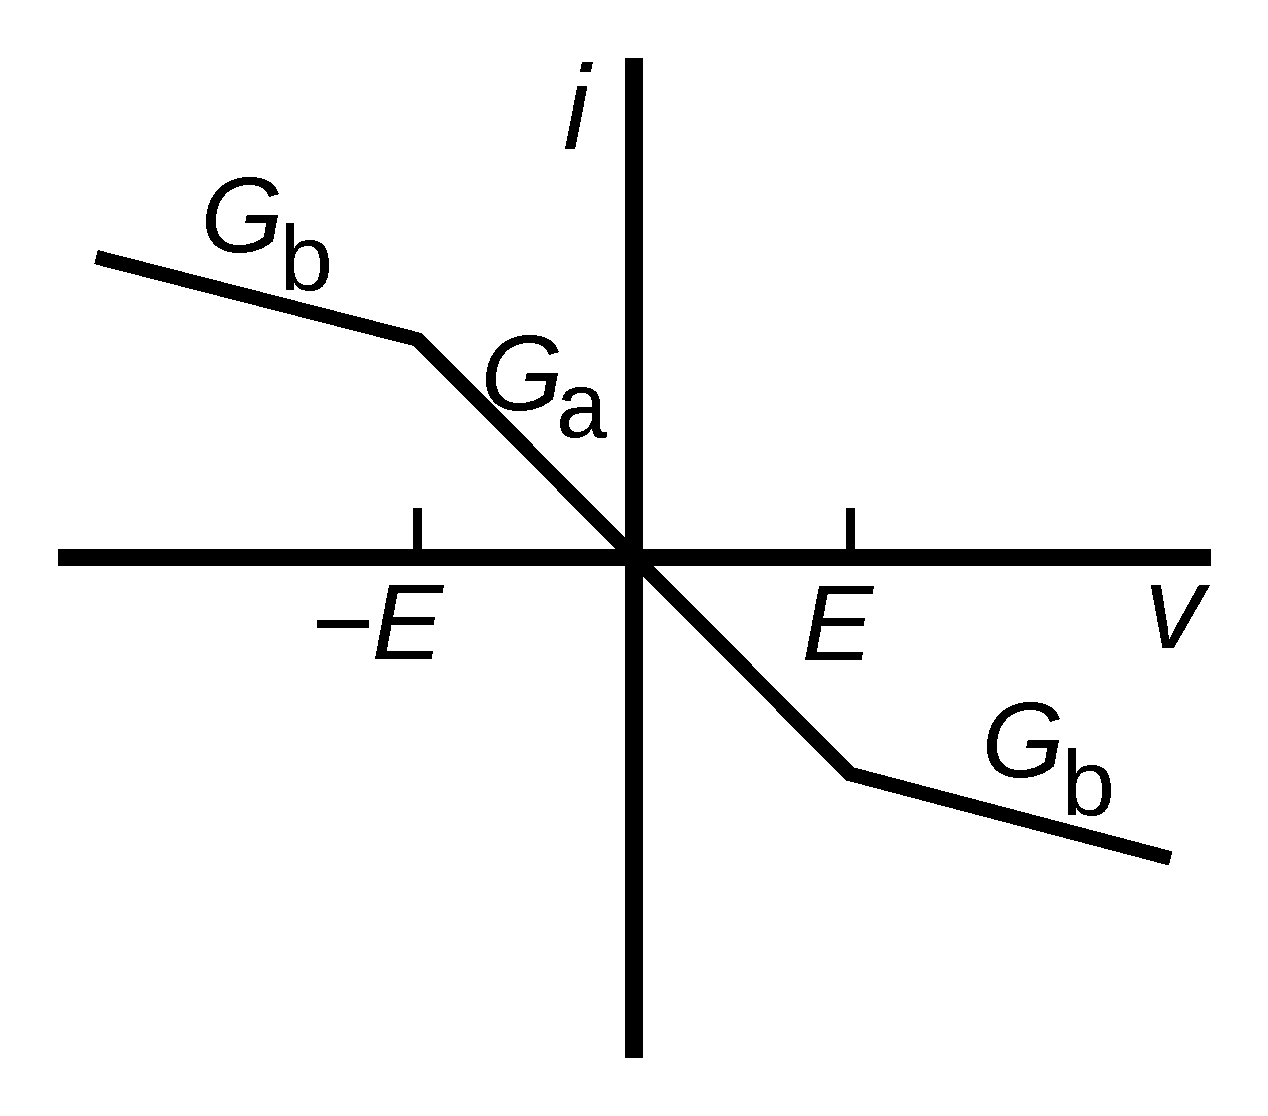
\includegraphics[width=0.49\textwidth]{controllers/chua-circuit/Chua-diode-characteristic-curve.pdf}
\caption[The Chua circuit]{The Chua circuit with its special Chua diode. The Chua diode is a piecewise-linear resistor with the characteristics as shown in the right figure.}
\label{figure:chuacircuit}
\end{figure}

Using Kirchhoff's circuit laws to derive the equations of the Chua circuit, we find the following non-linear ordinary differential equations with the variables x(t), y(t) and z(t).

\begin{align*}
\frac{dx}{dt}&=\alpha (y-x-f(x)) &\frac{dx}{dt}\text{ is the voltage across the capacitor }C_1\\
RC_2\frac{dy}{dt}&= (x-y+Rz) &\frac{dy}{dt}\text{ is the voltage across the capacitor }C_2\\
\frac{dy}{dt}&=\beta (x-y+Rz) &\text{with } \frac{1}{RC_2} \text{ being }\beta\\
\frac{dz}{dt}&=-\gamma y &\frac{dz}{dt}\text{ is the current across the inductor }L_1\\
f (x) &= \frac{m_1 x + (m_0 - m_1)}{2 (| x + E | -| x - E |)} &f(x)\text{ describes the response of the piecewise linear resistor}
\end{align*}

The Chua circuit was chosen as a model system of a chaotic controller because of its simple definition through the equations as well as it being a prior example system for simple limiter control in \cite{bib:Corron2000}. %
%
Corron et al. showed in two different chaotic systems, namely in the driven chaotic pendulum and the Chua circuit, how appropriate simple limiters can be applied to each system so that the chaotic behavior of each unbounded system could be controlled into behaviors of different periodicities. %
%
Important to mention is that the Chua Circuit is not meant to be a model for appropriate leg movement. %
%
The goal is to show that using simple limiters to control an arbitrary chaotic system, the different periodicities generated by the system leading to periodic leg movement could form different locomotion gaits. %
%
The change of the terrain representing a change of the simple limiters can lead to a change in periodic movement, thereby adaption to different environments occurs. 

\subsubsection{Simple Limiter Control in Mathematica}
\label{subsubsec:simple-limiter-mathematica}
%rev. 1

Before the circuit was used as a chaotic controller, it was modelled in Mathematica to observe its original chaotic behavior and influence it by simple limiters to exhibit different periodicities. %
%
Two experiments were conducted to look at two different limiter configurations in detail. %
%
One experiment explores the features of a self-limiting dimension and a dimension limiting another dimension. %
%
Another experiment reveals the influence of softness of the limiter on the control behavior in both of them. %
%
The differential equations were integrated using a Runge-Kutta integration scheme of order 6 with an integration step of \(h=0.001\). %
%
The constants were set as \(\alpha = 15.6\), \(\beta = 1\), \(\gamma = 28\), \(m_0 = -0.714\), \(m_1 = -1.143\) and \(E = 1\). %
%
The figure \ref{figure:chaoticchuacircuit} shows the Chua circuit's multiscroll attractor using initial conditions \((x(0),y(0),z(0)) = (-1.5,0,0)\) without any limiter. %
%
These initial conditions are used during the following experiments unless otherwise stated.

\begin{figure}[H]
\centering
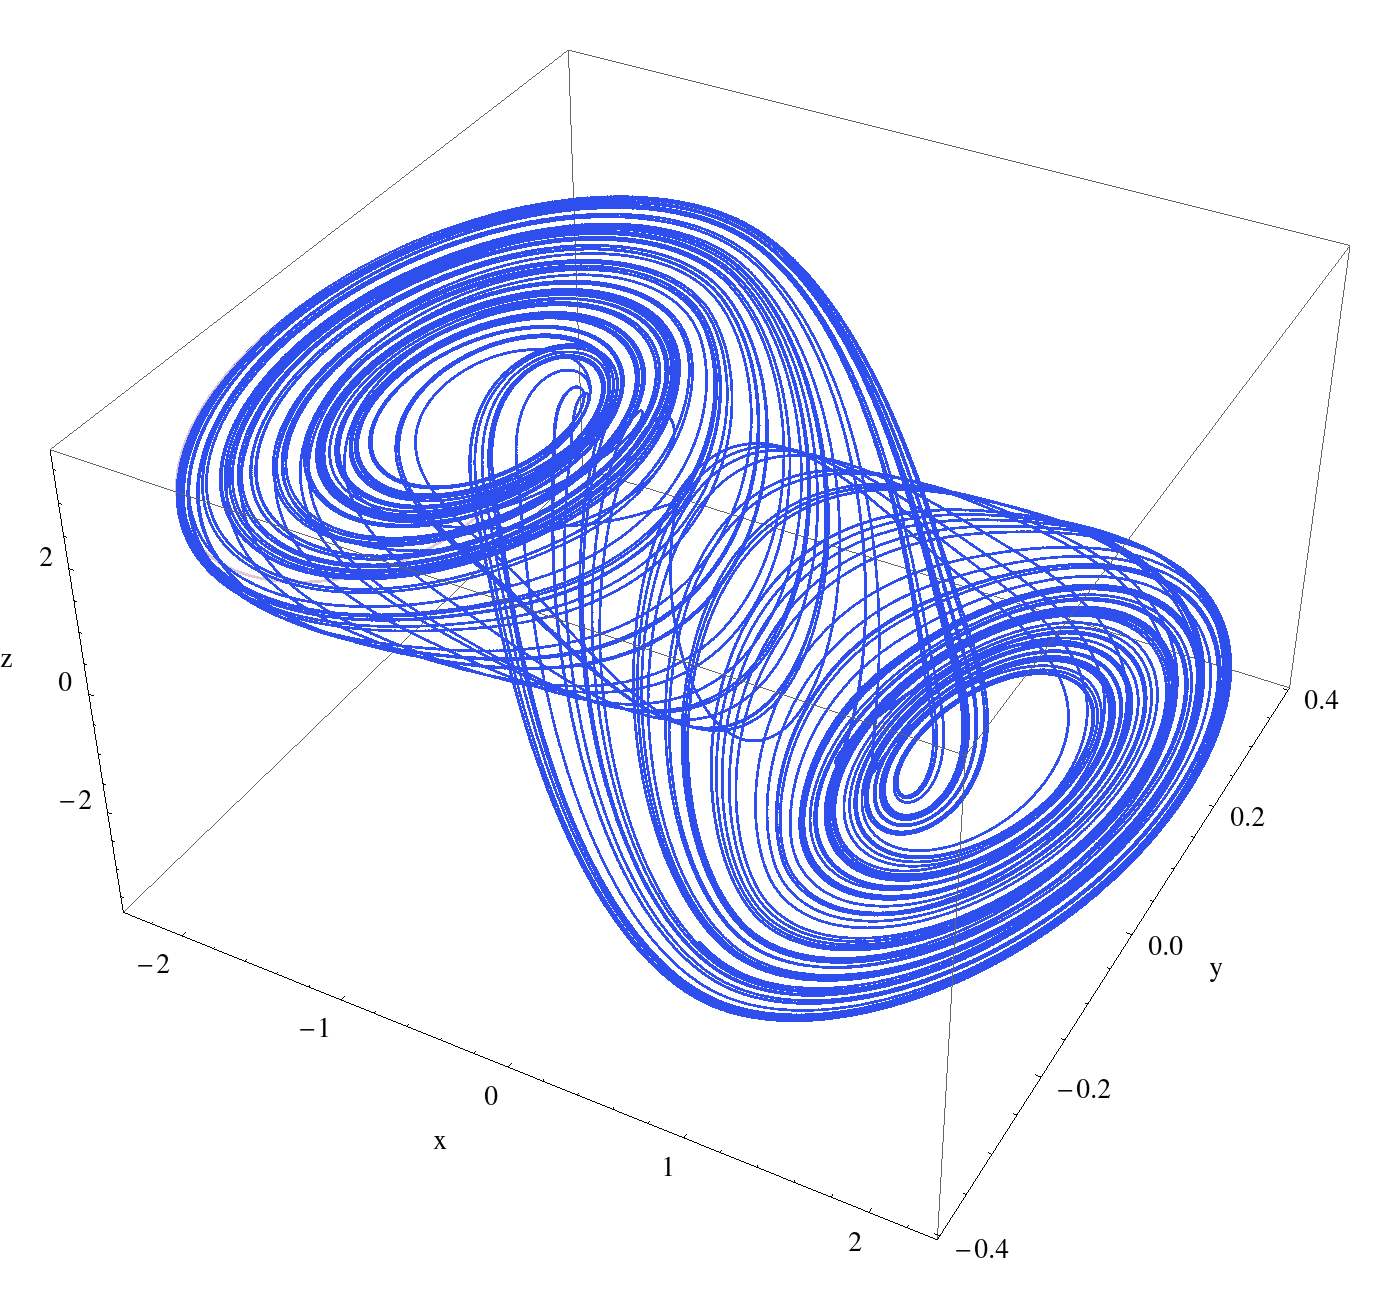
\includegraphics[width=0.8\textwidth]{controllers/chua-circuit/Unlimited-chua-circuit.png}
\caption[The multiscroll attractor in the Chua circuit]{The multiscroll attractor generated by the Chua circuit without any simple limiter applied.}
\label{figure:chaoticchuacircuit}
\end{figure}

Then we introduce a simple tunable soft limiter \[\text{softLim}(x) = \frac{1}{2} \left(\tanh\left(\frac{limitValue - x}{softness}\right) + 1\right)\] with the limiter response shown in figure \ref{figure:softlimiterresponse}. %
%
The limiter function is applied to one of the differential equations of the chaotic system and pulls its result to zero as it or one of the other equations surpass the $limitValue$ depending on which equation is defined to be the one triggering the limiter and which is the one to be limited.
%
In all of the following plots, the color of a certain state in the plot indicates how strongly the limiter influences that state.

\begin{figure}[H]
\centering
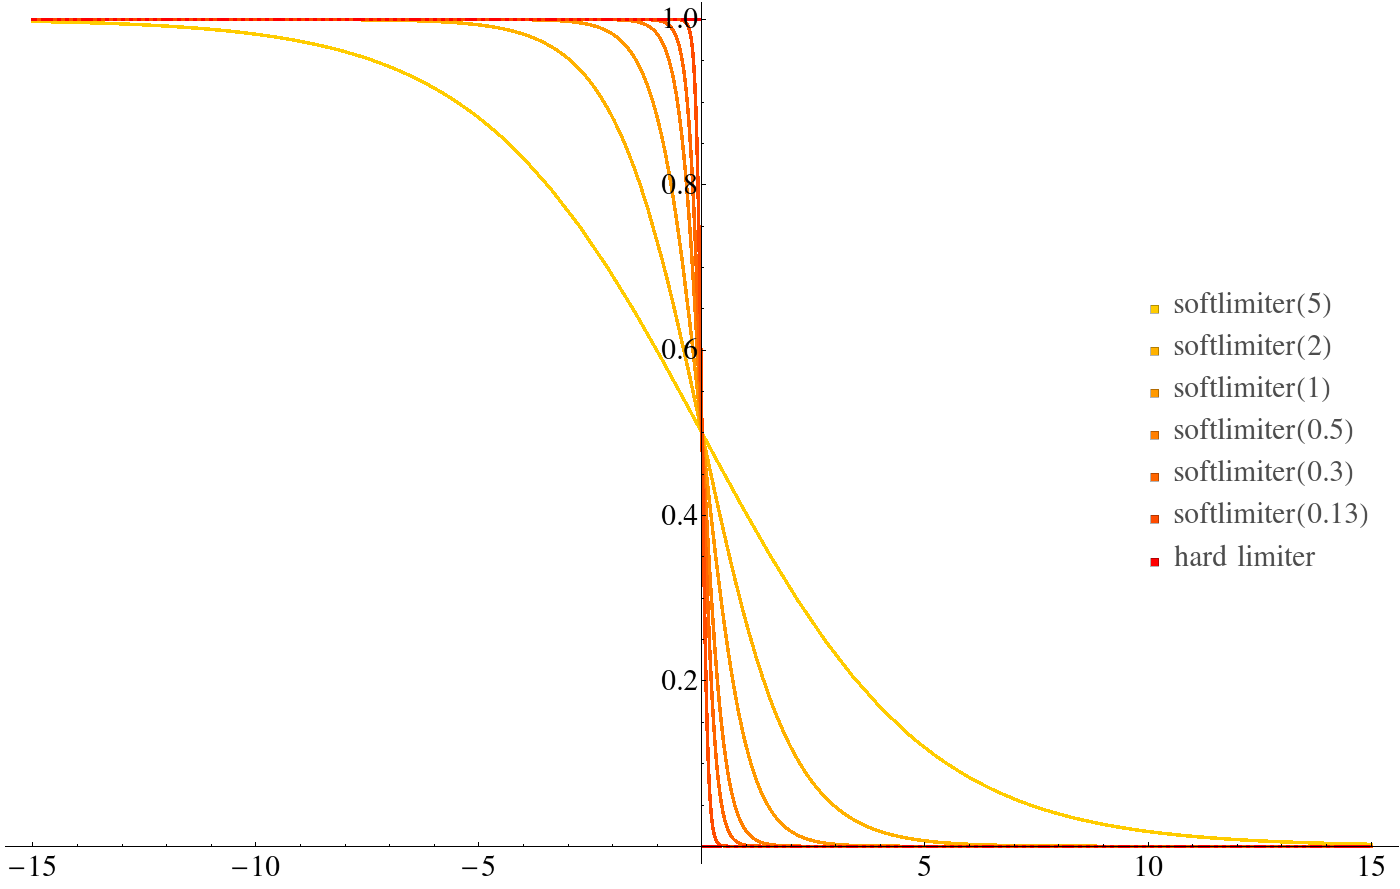
\includegraphics[width=0.8\textwidth]{controllers/chua-circuit/Limiter-softness-plot.png}
\caption[Soft limiter responses]{Soft limiter responses compared to the hard limiter response. The limiter function is applied to one of the differential equations of the chaotic system and pulls its result to zero as it or one of the others surpass the $limitValue$ depending on which equation is defined to be the one triggering the limiter and which is the one to be limited. The hard limiter response is shown in red. A trajectory approaching 0 from the negative side runs into the limiter, which applies the limiter instantly to its full extent. The soft limiter responses from orange to yellow show how limiters with increasing softness values (0.13, 0.3, 0.5, 1, 2 and 5) are applied. The curve with softness 0.13 approximates the hard limiter the best, the higher the softness value, the softer the limiter.}
\label{figure:softlimiterresponse}
\end{figure}

Initially a hard limiter defined as a piecewise function was chosen, however a soft limiter is a better model for physical limiters, because in reality no ideal hard limiters exist. %
%
Using the $softness$ parameter of the limiter, the softness can be tuned, where a \(softness = 10\) means very soft and a \(softness = 0.1\) signifies a very hard limiter. %
%
The $limitValue$ parameter defines the threshold value, at which the limiter is applied exactly half when surpassed. %
%
With the above mentioned initial conditions, the trajectory in state space stays within the bounding box of 

\begin{align*}
x &\in [-2.8717,2.2417]\\
y &\in [-0.380467,0.386978]\\
z &\in [-3.59156,3.62959]
\end{align*}

\paragraph{One Dimension Limiting Another}

In the first experiment, the softness was set to \(softness=0.13\) to approximate a rather hard limiter. The limiter is added to the equations as shown below:

\begin{align*}
\frac{dx}{dt}&=\alpha (y-x-f(x)) \\
\frac{dy}{dt}&=\beta (x-y + Rz)\\
\frac{dz}{dt}&=-\gamma ~ y ~ \text{softLim}(x)\\
f (x) &= \frac{m_1 x + (m_0 - m_1)}{2 (| x + E | -| x - E |)}
\end{align*}

If the $limitValue$ parameter is changed from \(>3.19\), which corresponds to no limiter influence to the trajectory, to a value within \(limitValue \in [2.28,3.19]\), different chaotic trajectories can be observed. %
%
The limiter influences the circuit by limiting the change of current flow \(\frac{dz}{dt}\) when \(x\) approaches the limiter.

\begin{figure}[H]
\centering
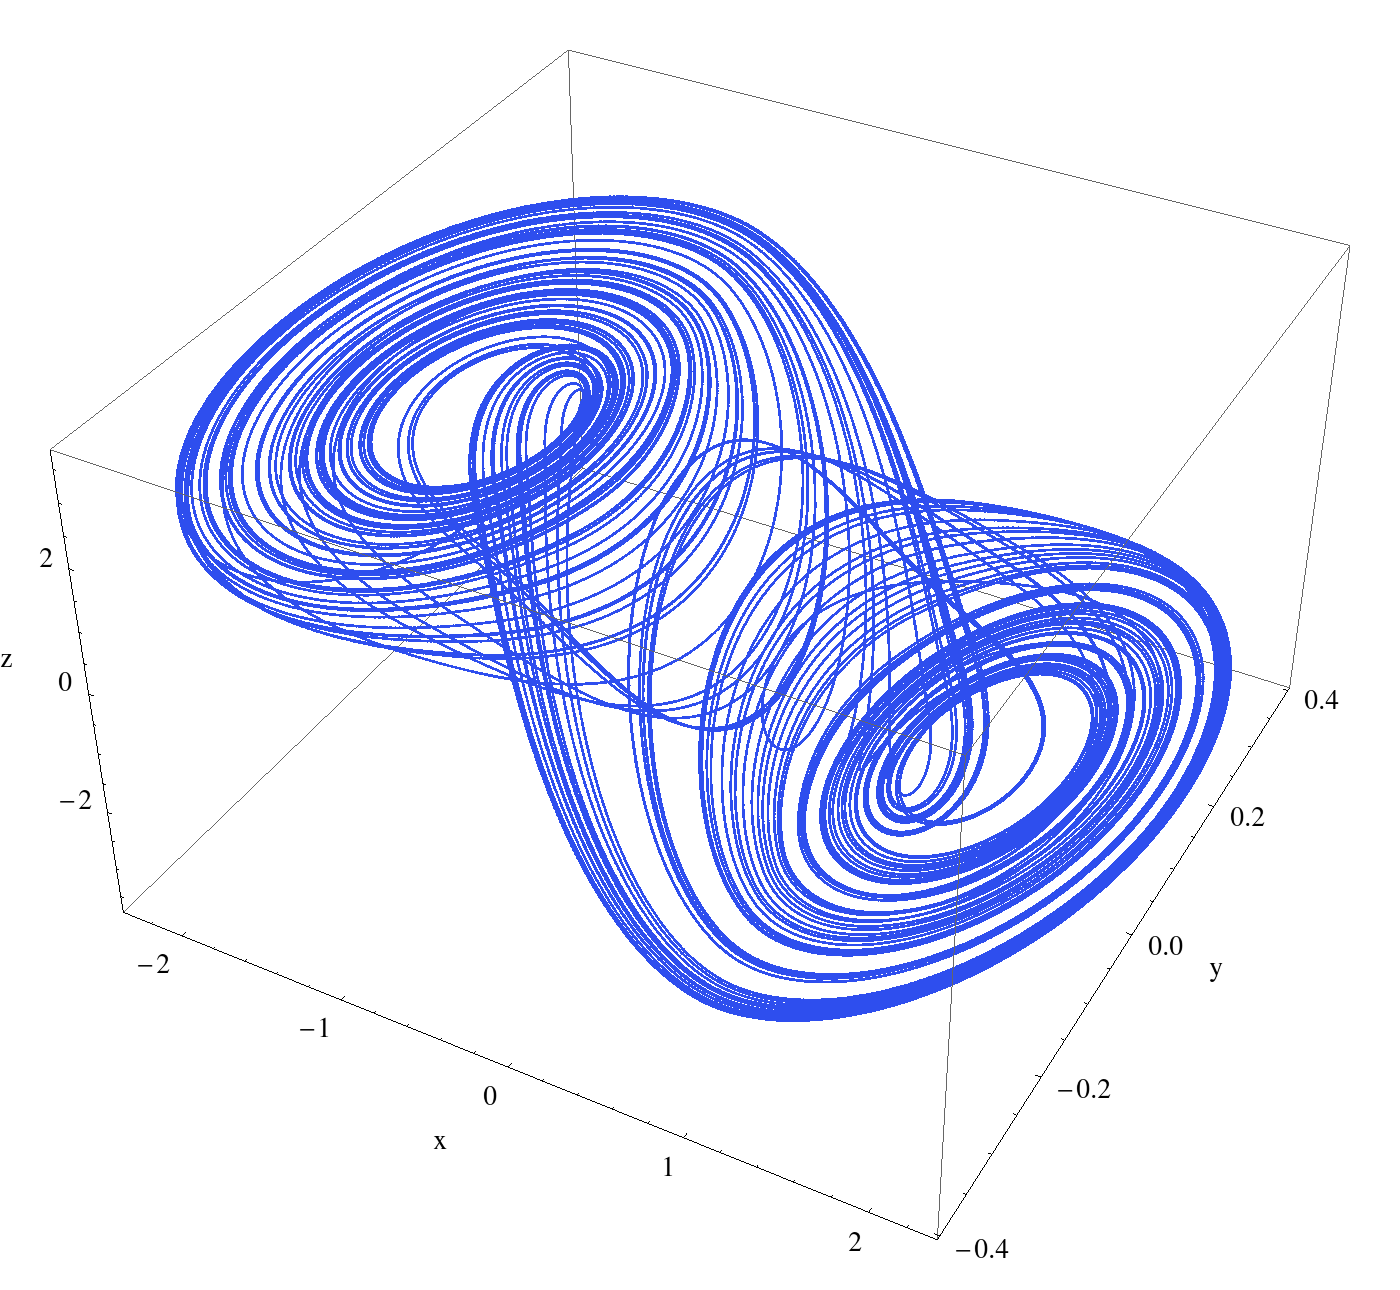
\includegraphics[width=0.45\textwidth]{controllers/chua-circuit/Limited-chua-circuit-z-softness-0-13-3.png}
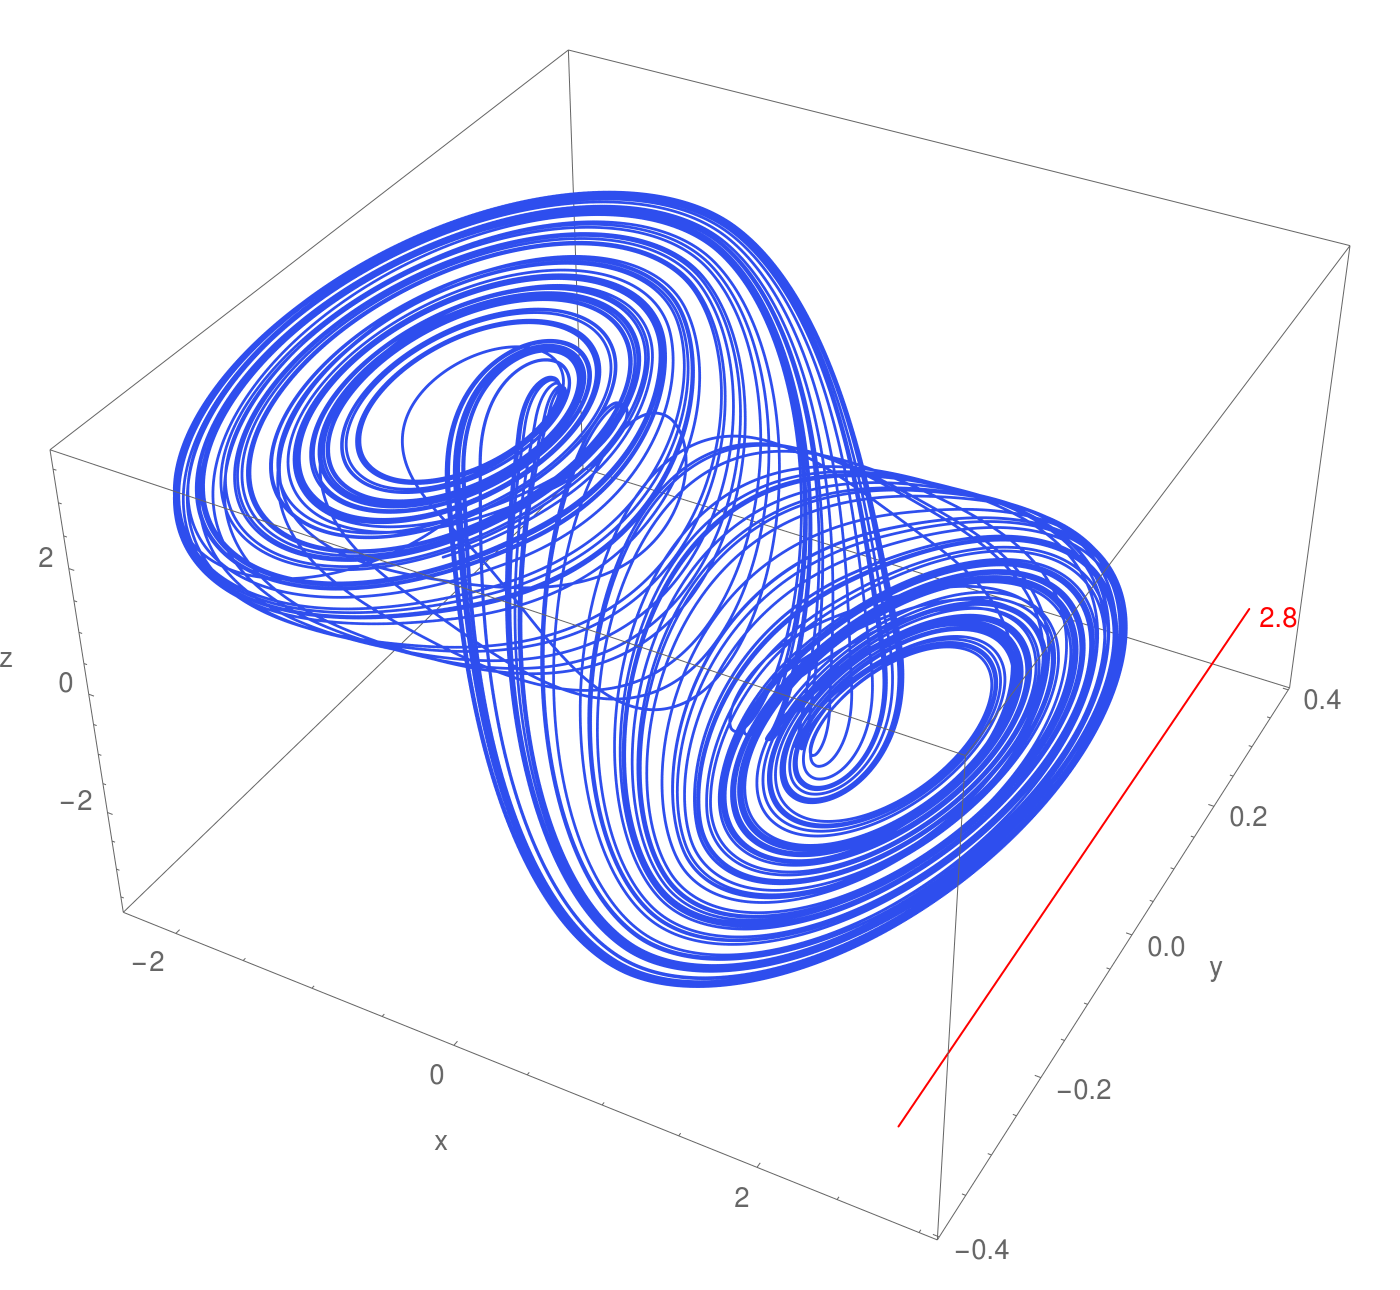
\includegraphics[width=0.45\textwidth]{controllers/chua-circuit/Limited-chua-circuit-z-softness-0-13-2-8.png}
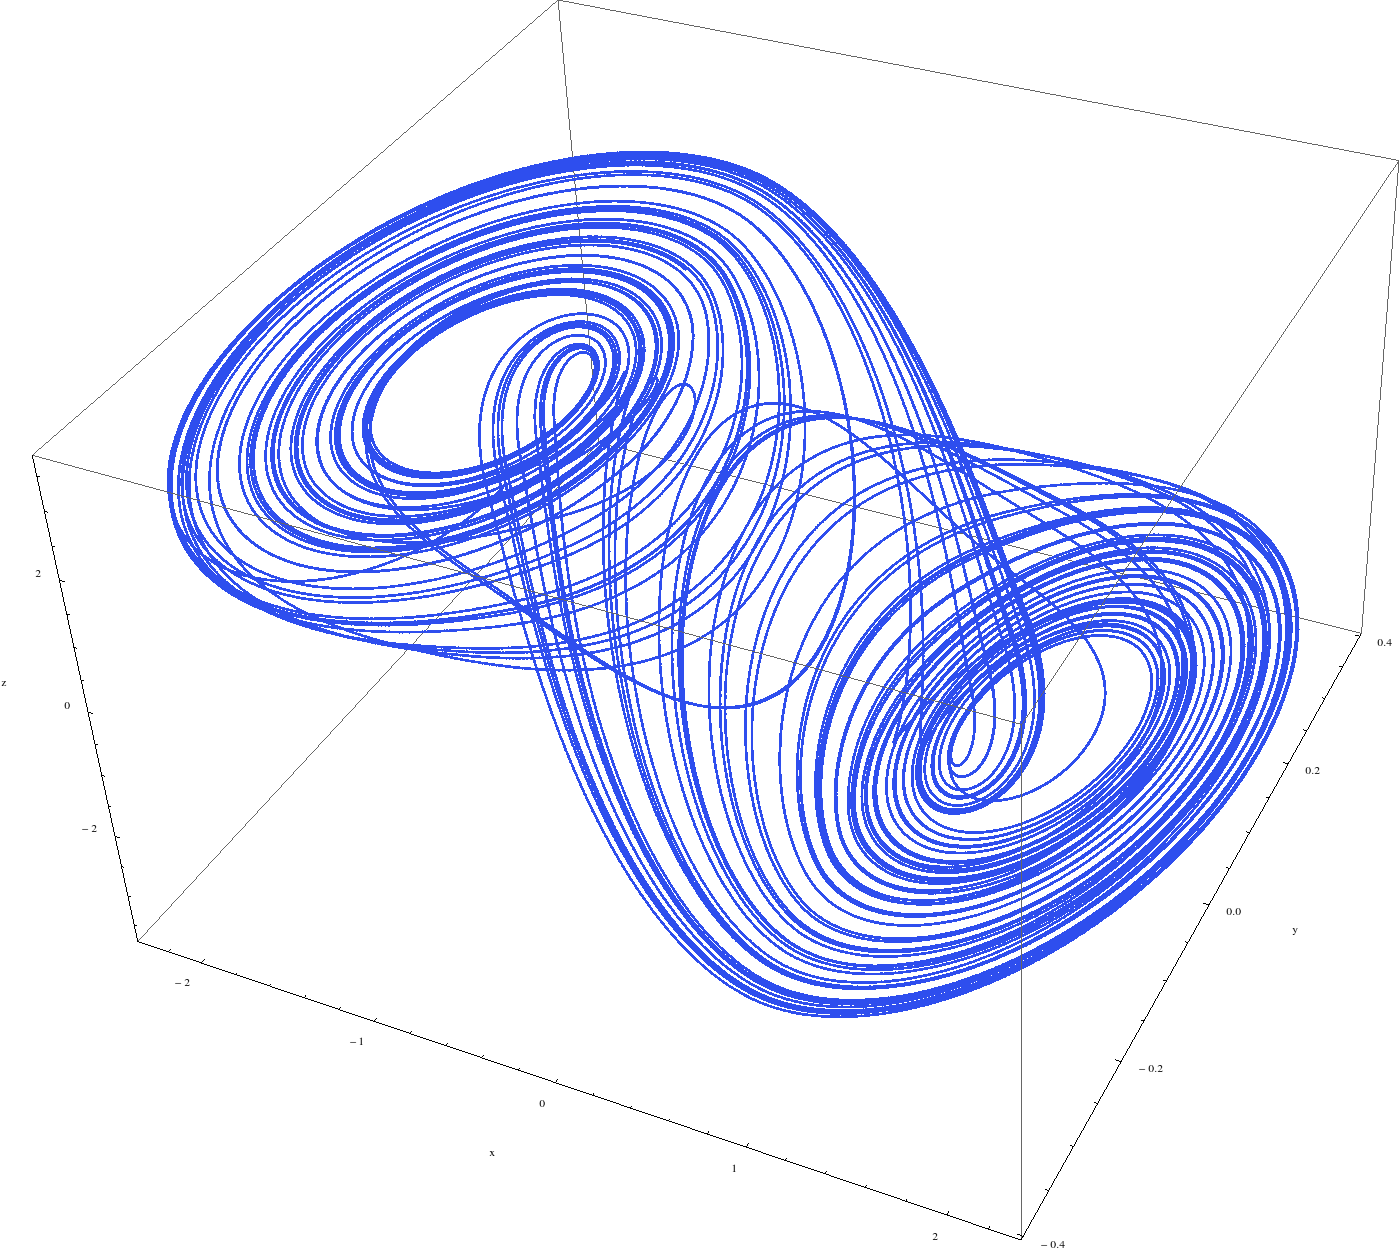
\includegraphics[width=0.45\textwidth]{controllers/chua-circuit/Limited-chua-circuit-z-softness-0-13-2-6.png}
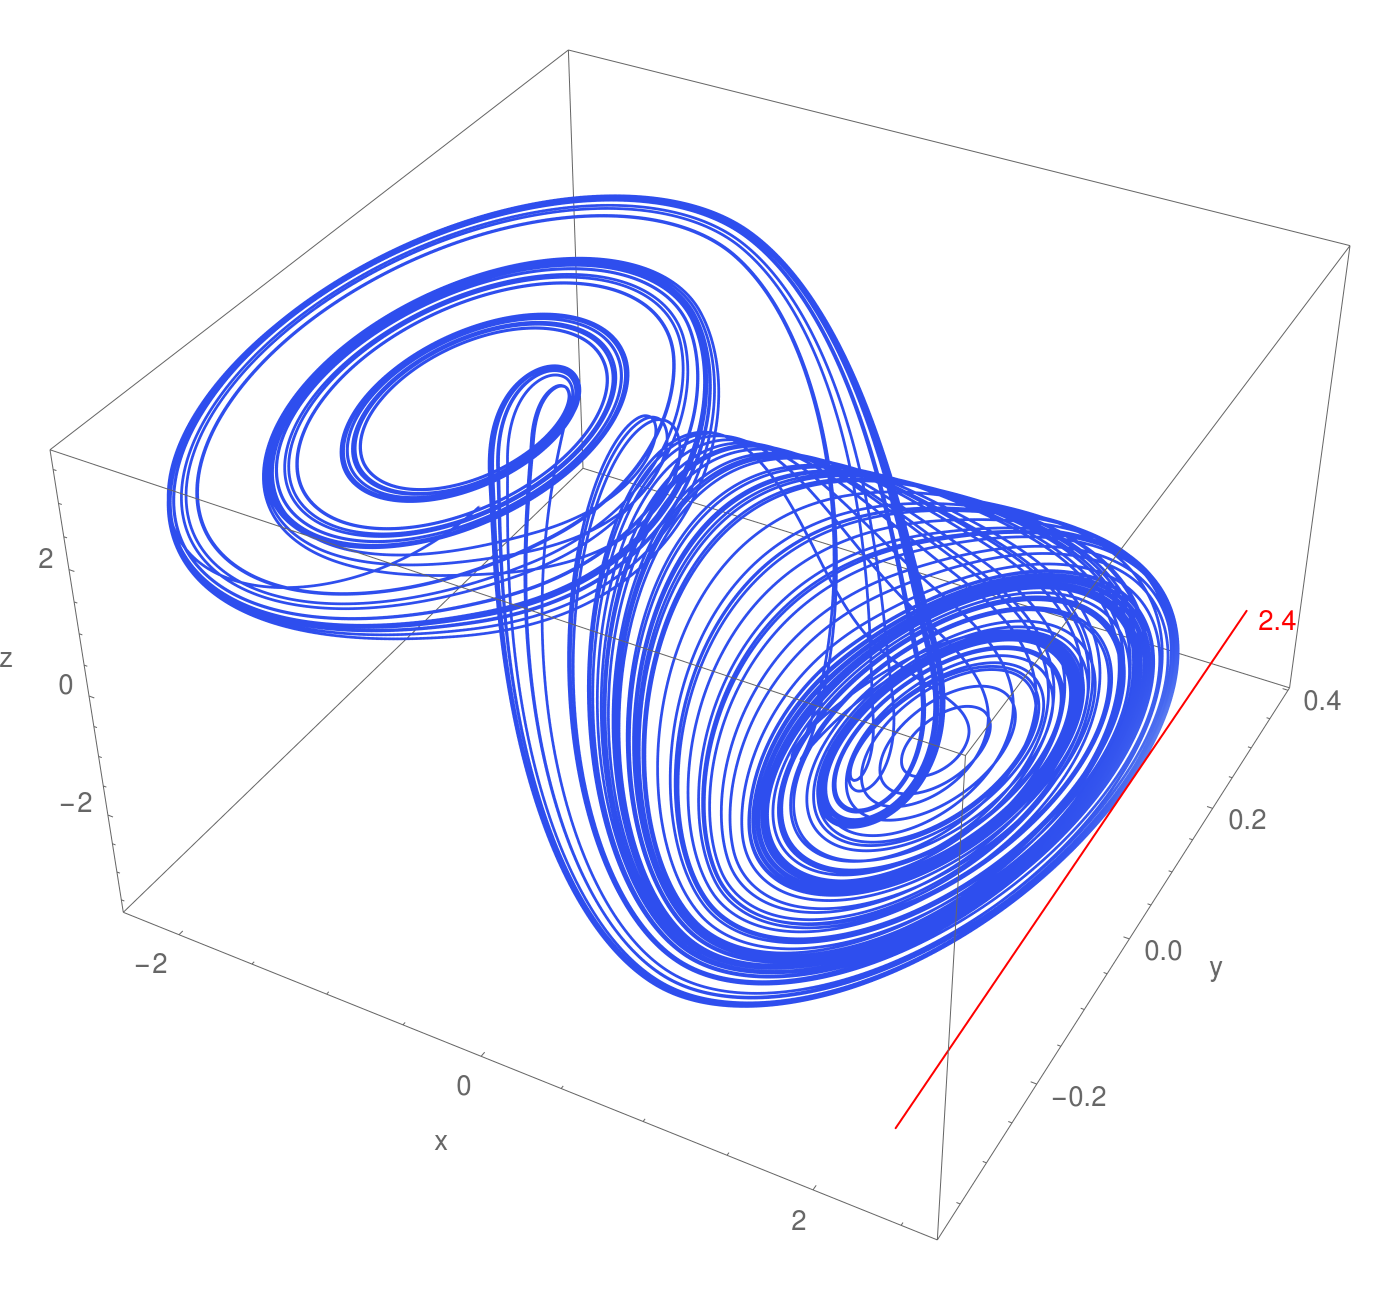
\includegraphics[width=0.45\textwidth]{controllers/chua-circuit/Limited-chua-circuit-z-softness-0-13-2-4.png}
\caption[Figure of chaotic behaviors in range 2.4-3.19]{Figure of chaotic behaviors in range 2.4-3.19. The limit values of the shown figures are \(3\), \(2.8\), \(2.6\) and \(2.4\).}
\label{figure:z-2.4-3.19-chaotictrajectories}
\end{figure}

When choosing a \(limitValue \in [2.28,2.4[\), one can observe that the limiter more and more suppresses chaotic behavior and reduces the number of times the trajectory switches back into the uppermost scroll of the multiscroll.

\begin{figure}[H]
\centering
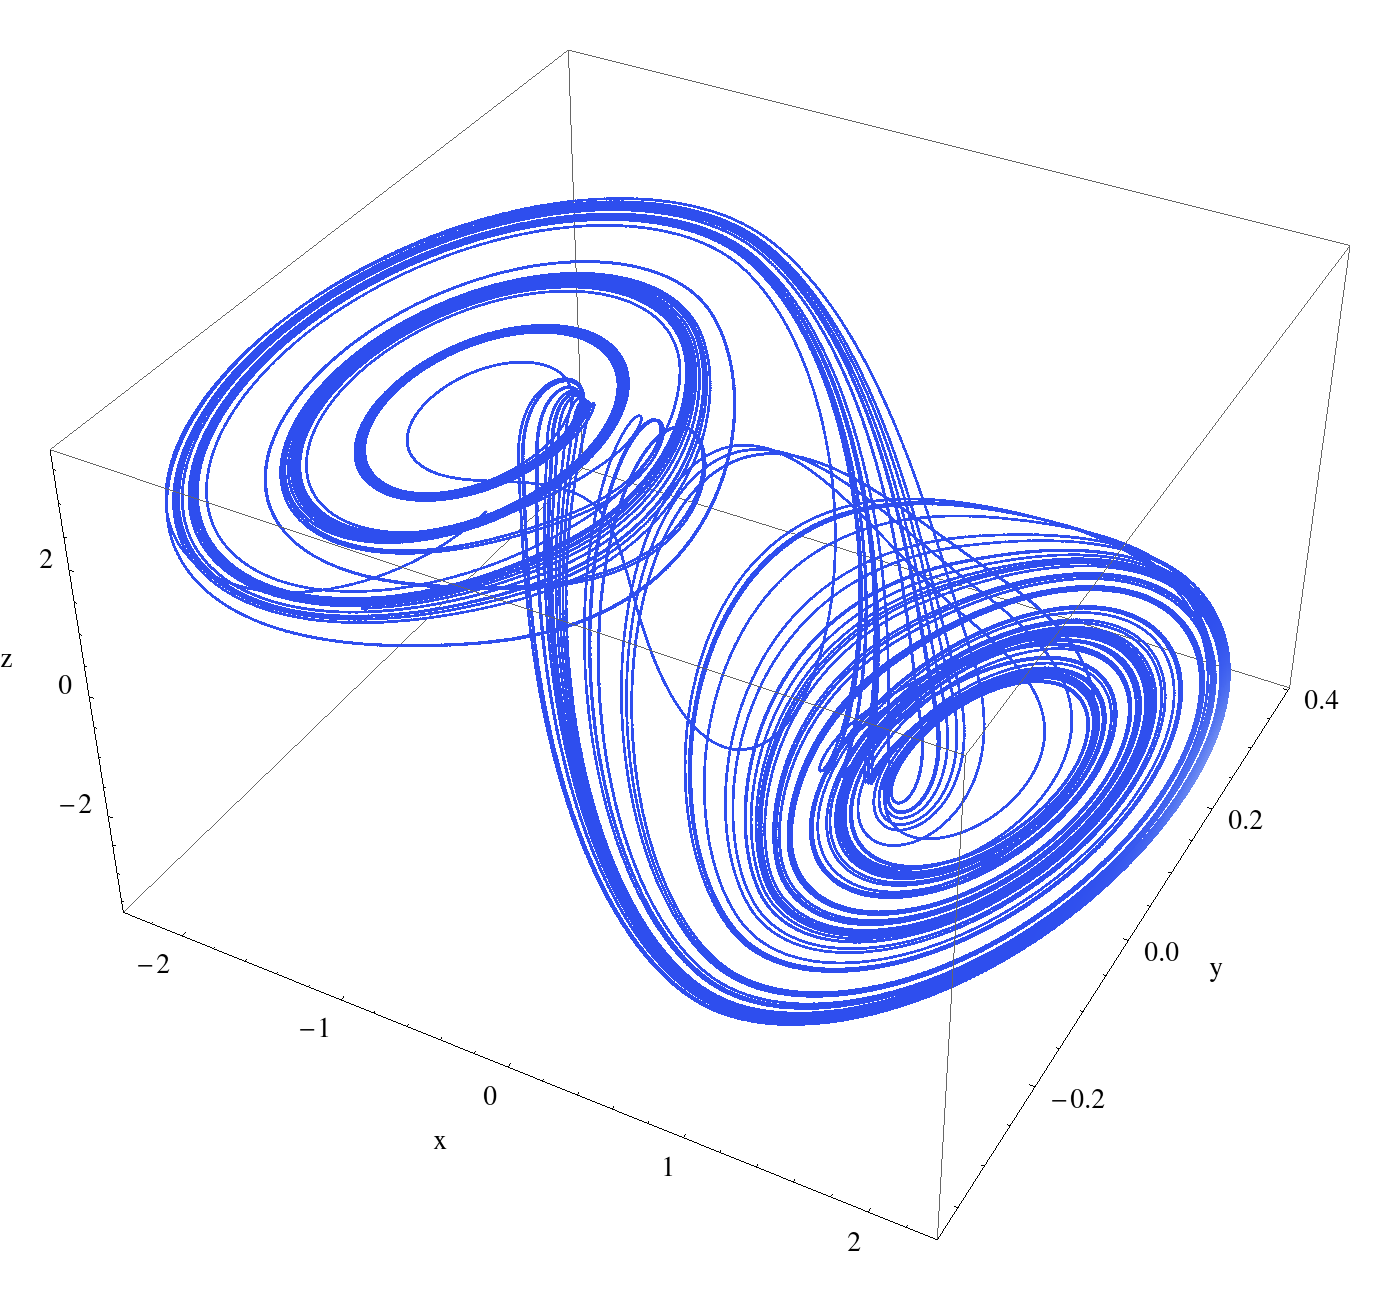
\includegraphics[width=0.45\textwidth]{controllers/chua-circuit/Limited-chua-circuit-z-softness-0-13-2-375.png}
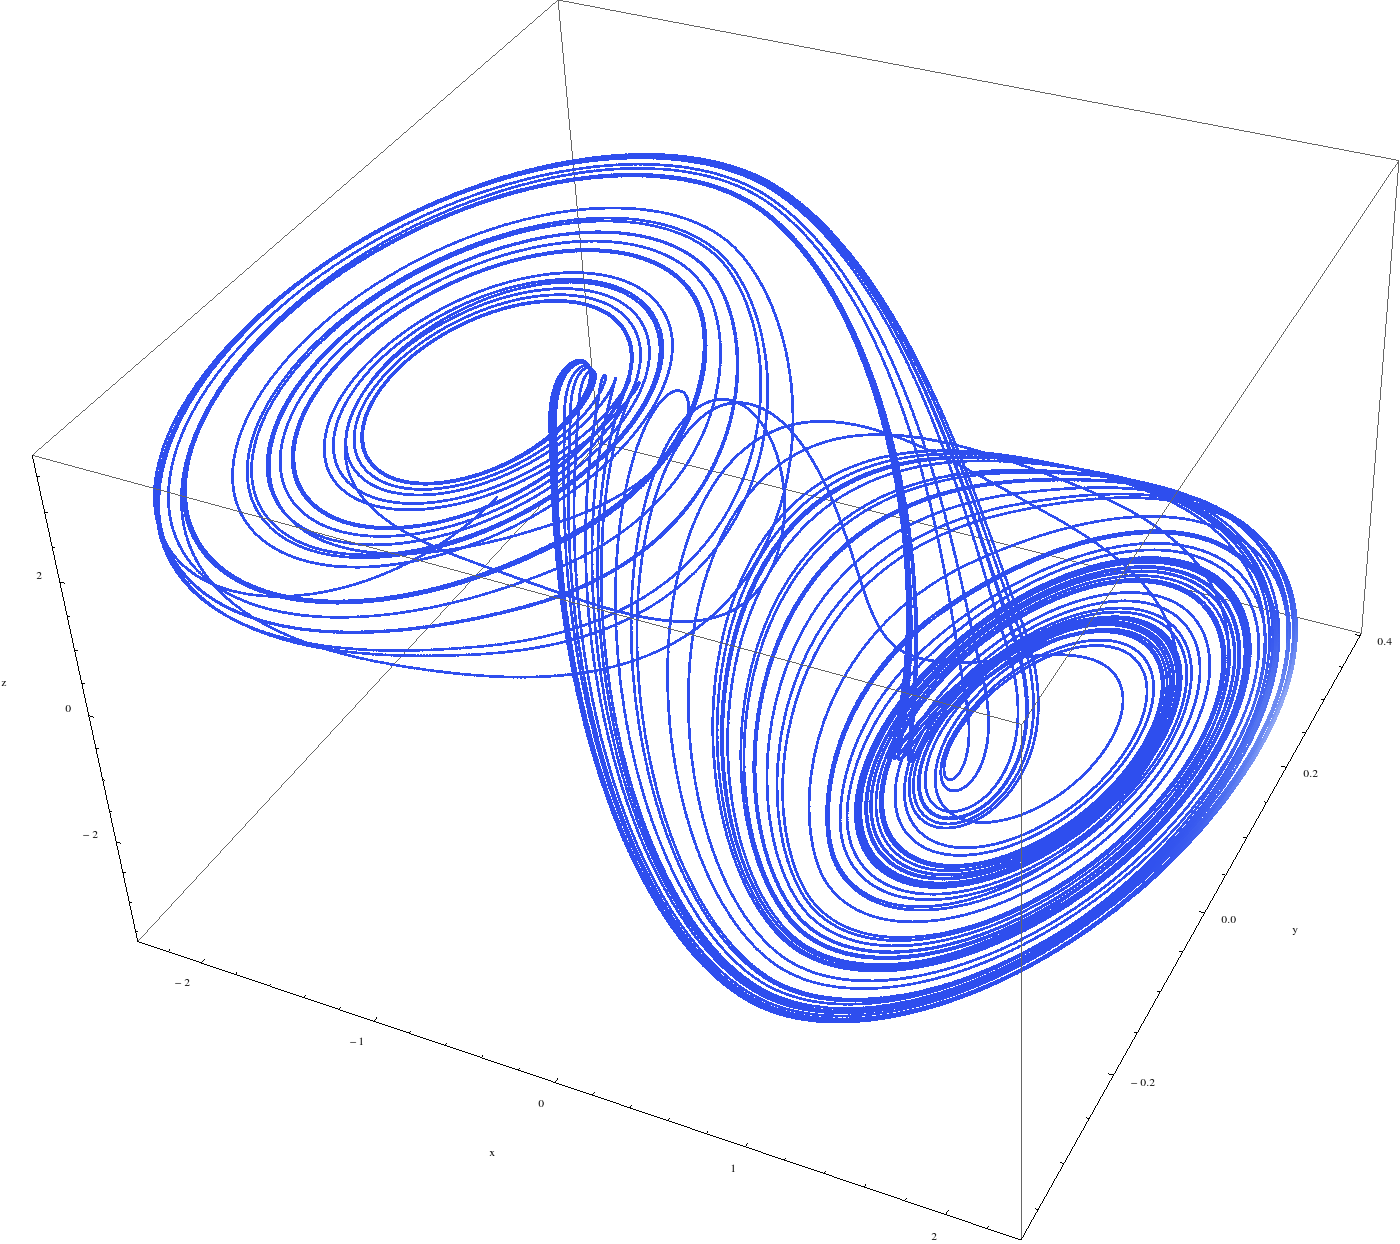
\includegraphics[width=0.45\textwidth]{controllers/chua-circuit/Limited-chua-circuit-z-softness-0-13-2-35125.png}
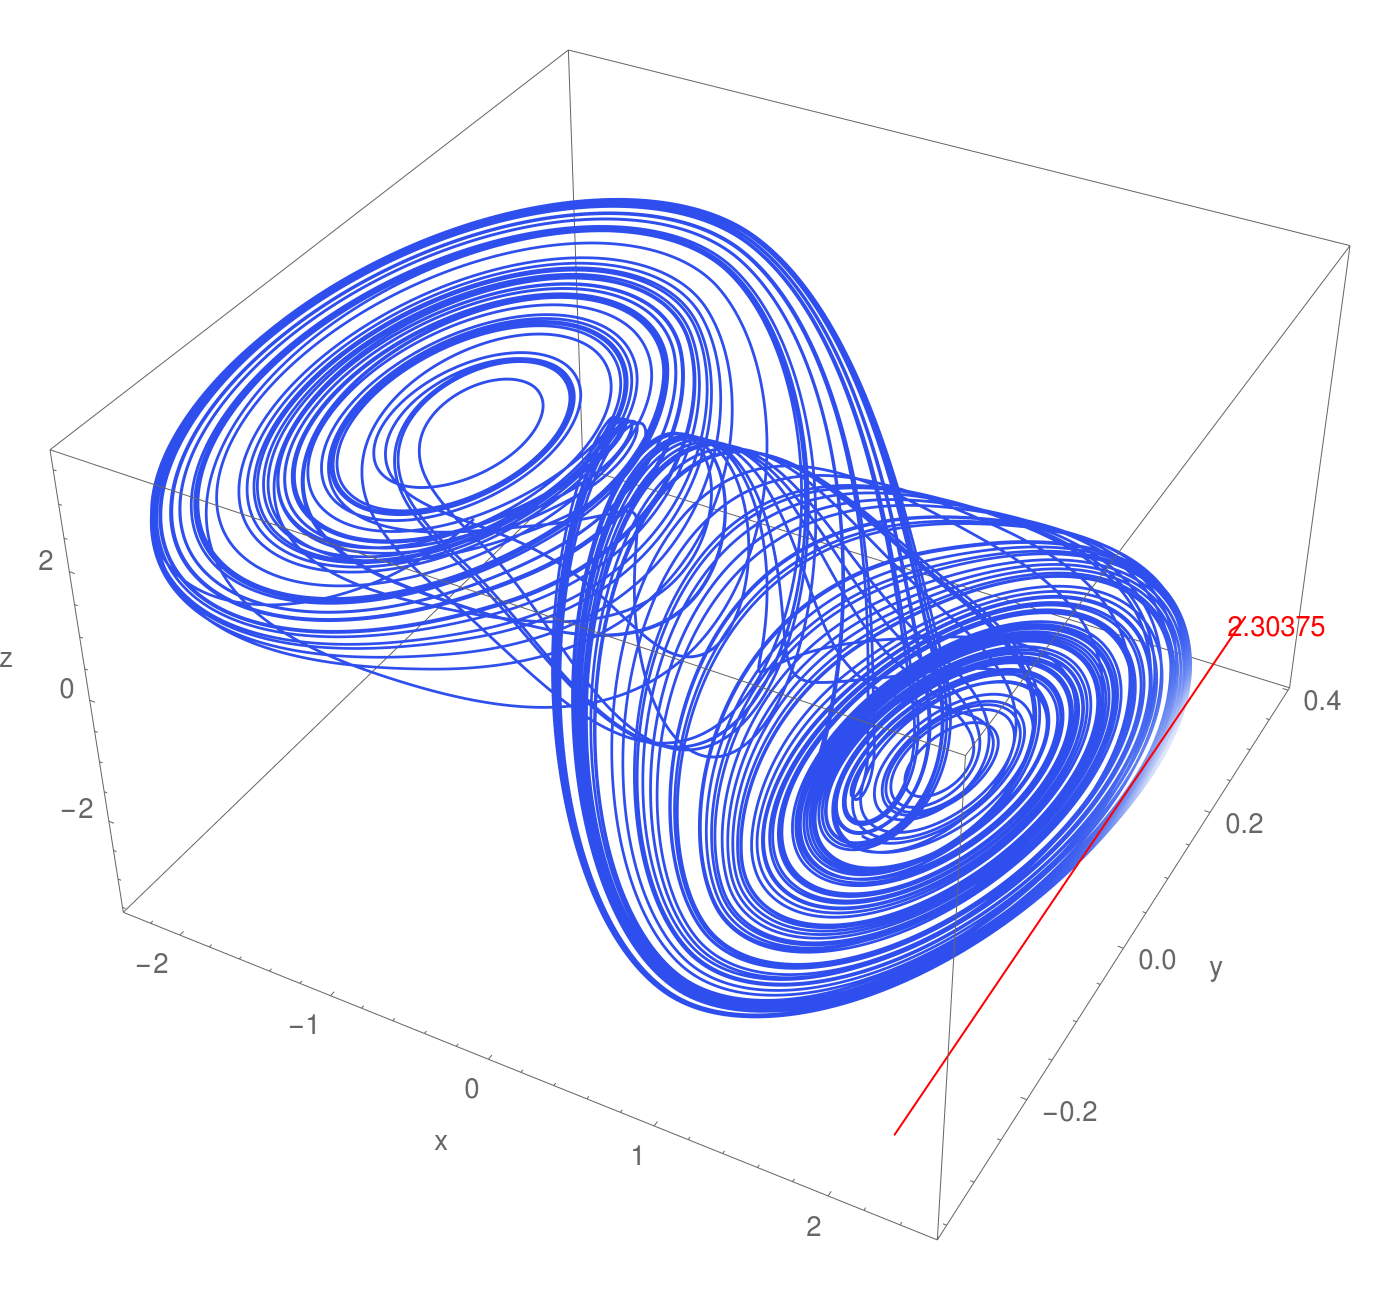
\includegraphics[width=0.45\textwidth]{controllers/chua-circuit/Limited-chua-circuit-z-softness-0-13-2-30375.png}
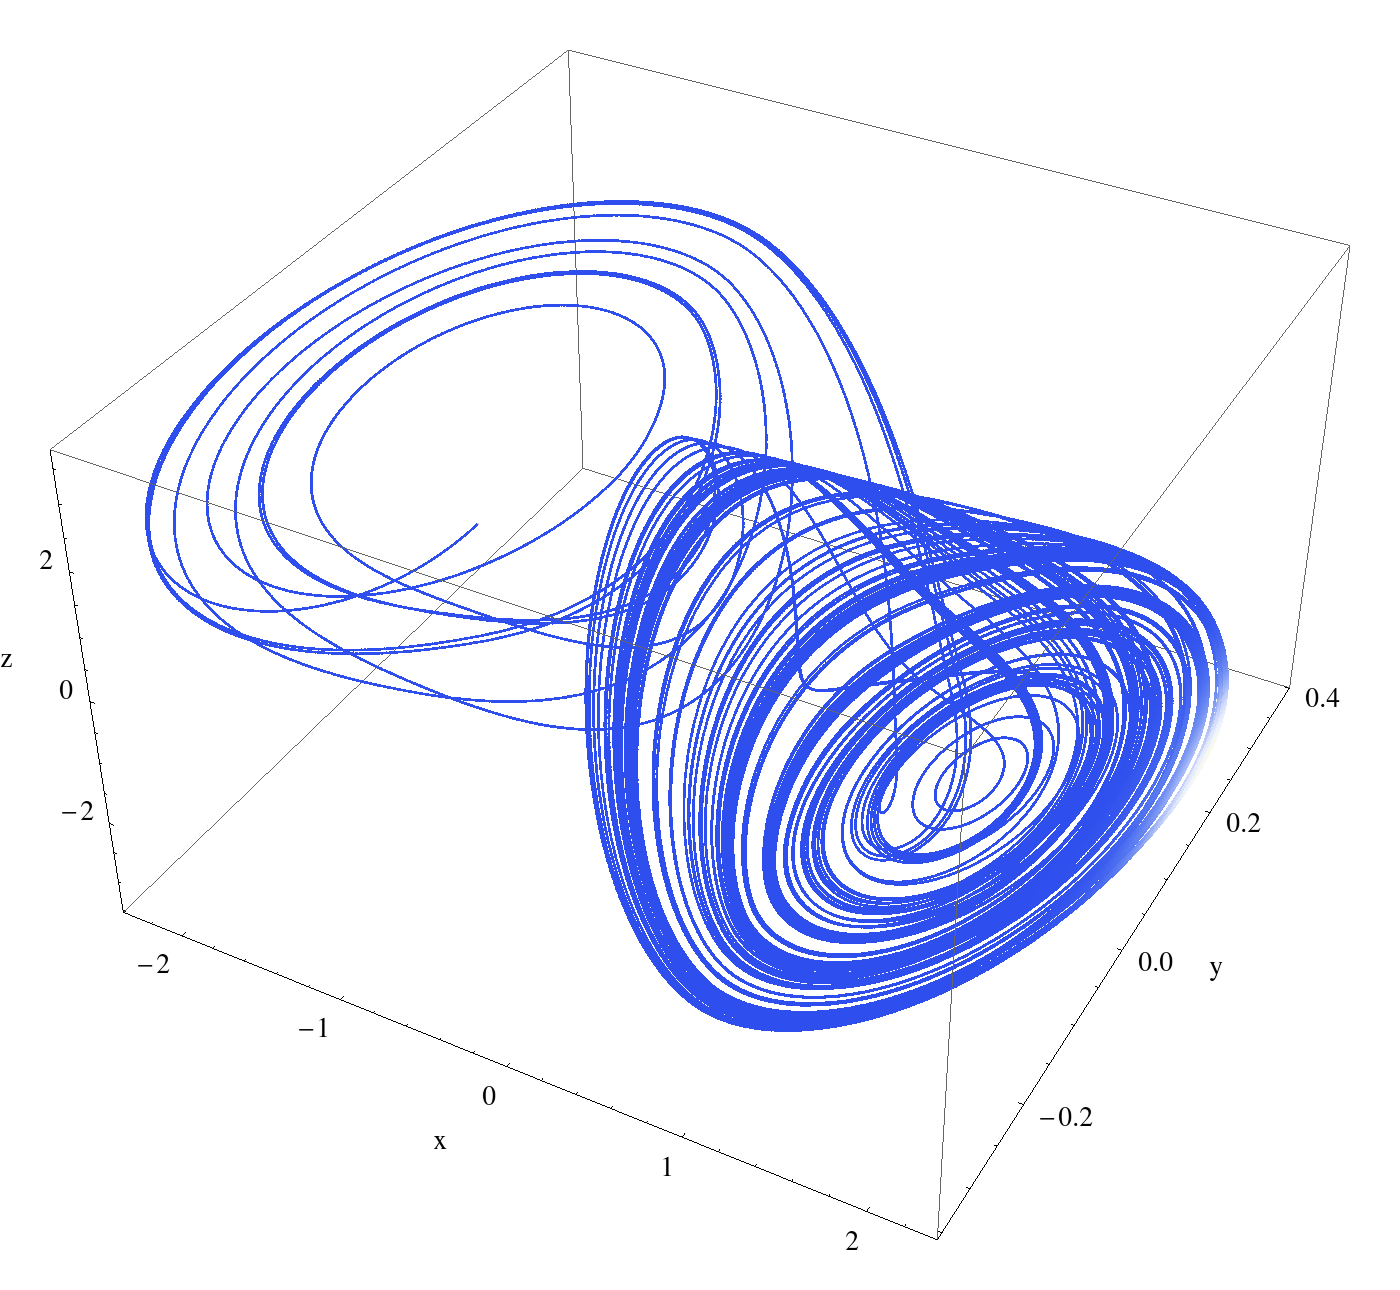
\includegraphics[width=0.45\textwidth]{controllers/chua-circuit/Limited-chua-circuit-z-softness-0-13-2-28.png}
\caption[Figure of behaviors in range 2.28-2.4]{Figure of behaviors in range 2.28-2.4. The limit values of the shown figures are \(2.375\), \(2.35125\), \(2.30375\) and \(2.28\). In the lower left and right plot, the slightly white coloring of the curve indicates the strength of the limiter influence.}
\label{figure:z-2.28-2.4-chaotictrajectories}
\end{figure}

With a value of \(limitValue \in [1.81, 2.28]\), the state only stays in the lowermost scroll and shows periodic behavior. %
%
The control behavior can be explained by looking at figure \ref{figure:chaoticchuacircuit} again. %
%
The trajectories that lead from the lower-most scroll to the upper-most scroll pass by at the outer orbits of the lower-most scroll and therefore have the highest x(t) values. %
%
The limiter is applied when a certain x(t) value is surpassed, therefore the limiter limits z(t), which then leads to a repelling influence from the limiter. %
%
The trajectory thereby is pulled back onto a former orbit, which stabilizes the state onto that orbit. %
%
However, since the limiter is a very hard limiter, the period of the trajectory shows higher periods only in a very small limit value parameter window \([2.212,2.215]\) and then very quickly turns into period 1 within the parameter window \([1.83,2.212]\) with quicker convergence the nearer the limiter was placed to zero. %
%
The system is highly sensitive to the exact position of the limiter because of the dense periodic orbits in the system, between which the state quickly switches when the limiter is slightly moved. %
%
One can see the convergence to the limit cycle vary, getting slower again with \(limitValue \in [2.183,2.15]\) increasing again for \(limitValue \in [2.15,1.83]\). %
%
A self-similar pattern of increasing and decreasing convergence speeds can be observed.

\begin{figure}[H]
\centering
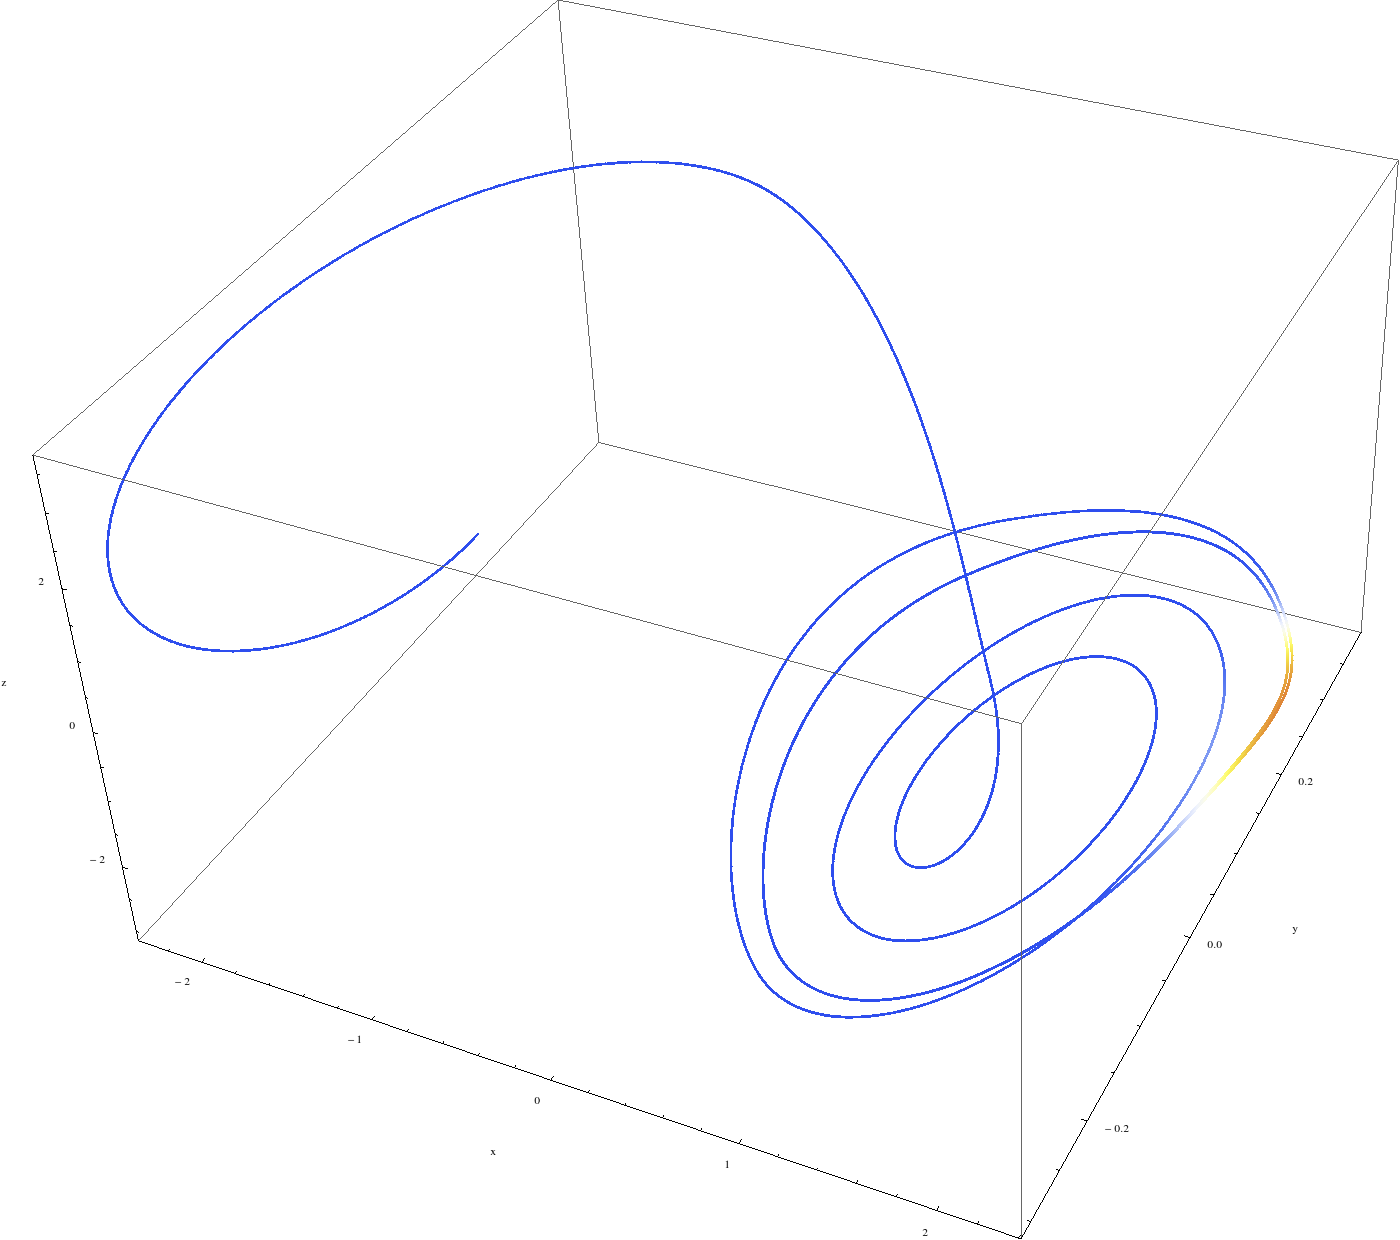
\includegraphics[width=0.45\textheight]{controllers/chua-circuit/Limited-chua-circuit-z-softness-0-13-2-183-convergence.png}
%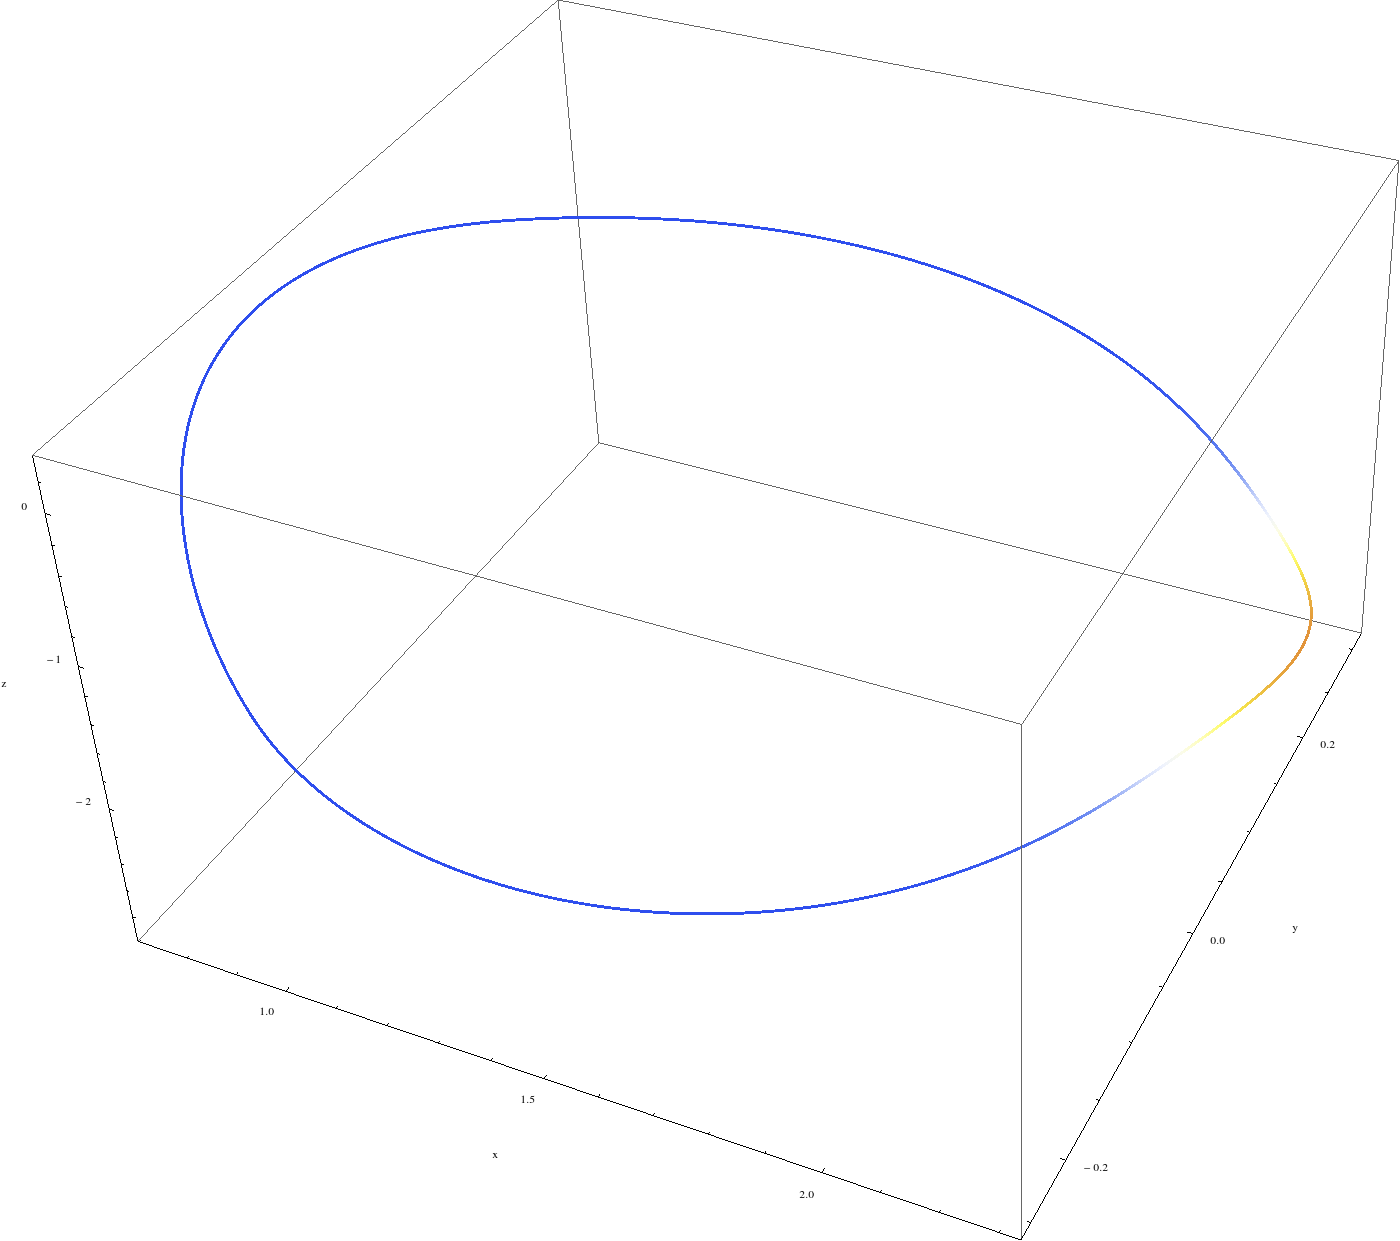
\includegraphics[width=0.45\textheight]{controllers/chua-circuit/Limited-chua-circuit-z-softness-0-13-2-183.png}

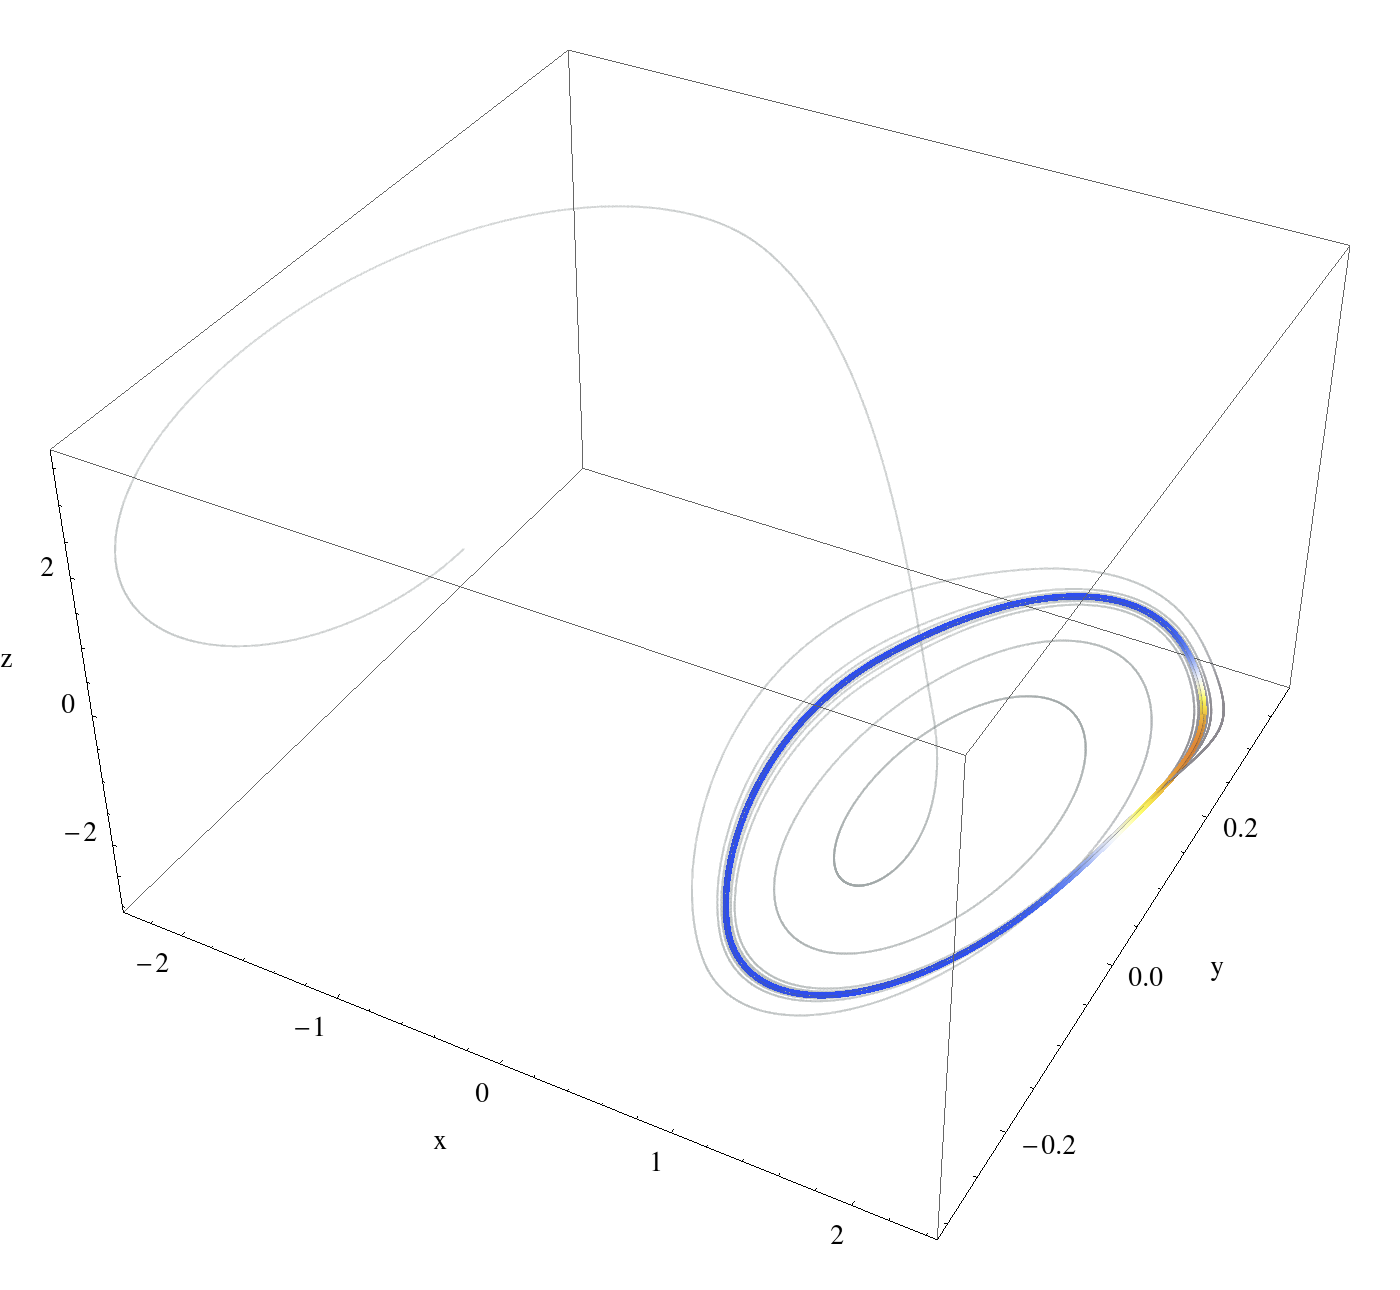
\includegraphics[width=0.45\textheight]{controllers/chua-circuit/Limited-chua-circuit-z-softness-0-13-2-15-convergence.png}
%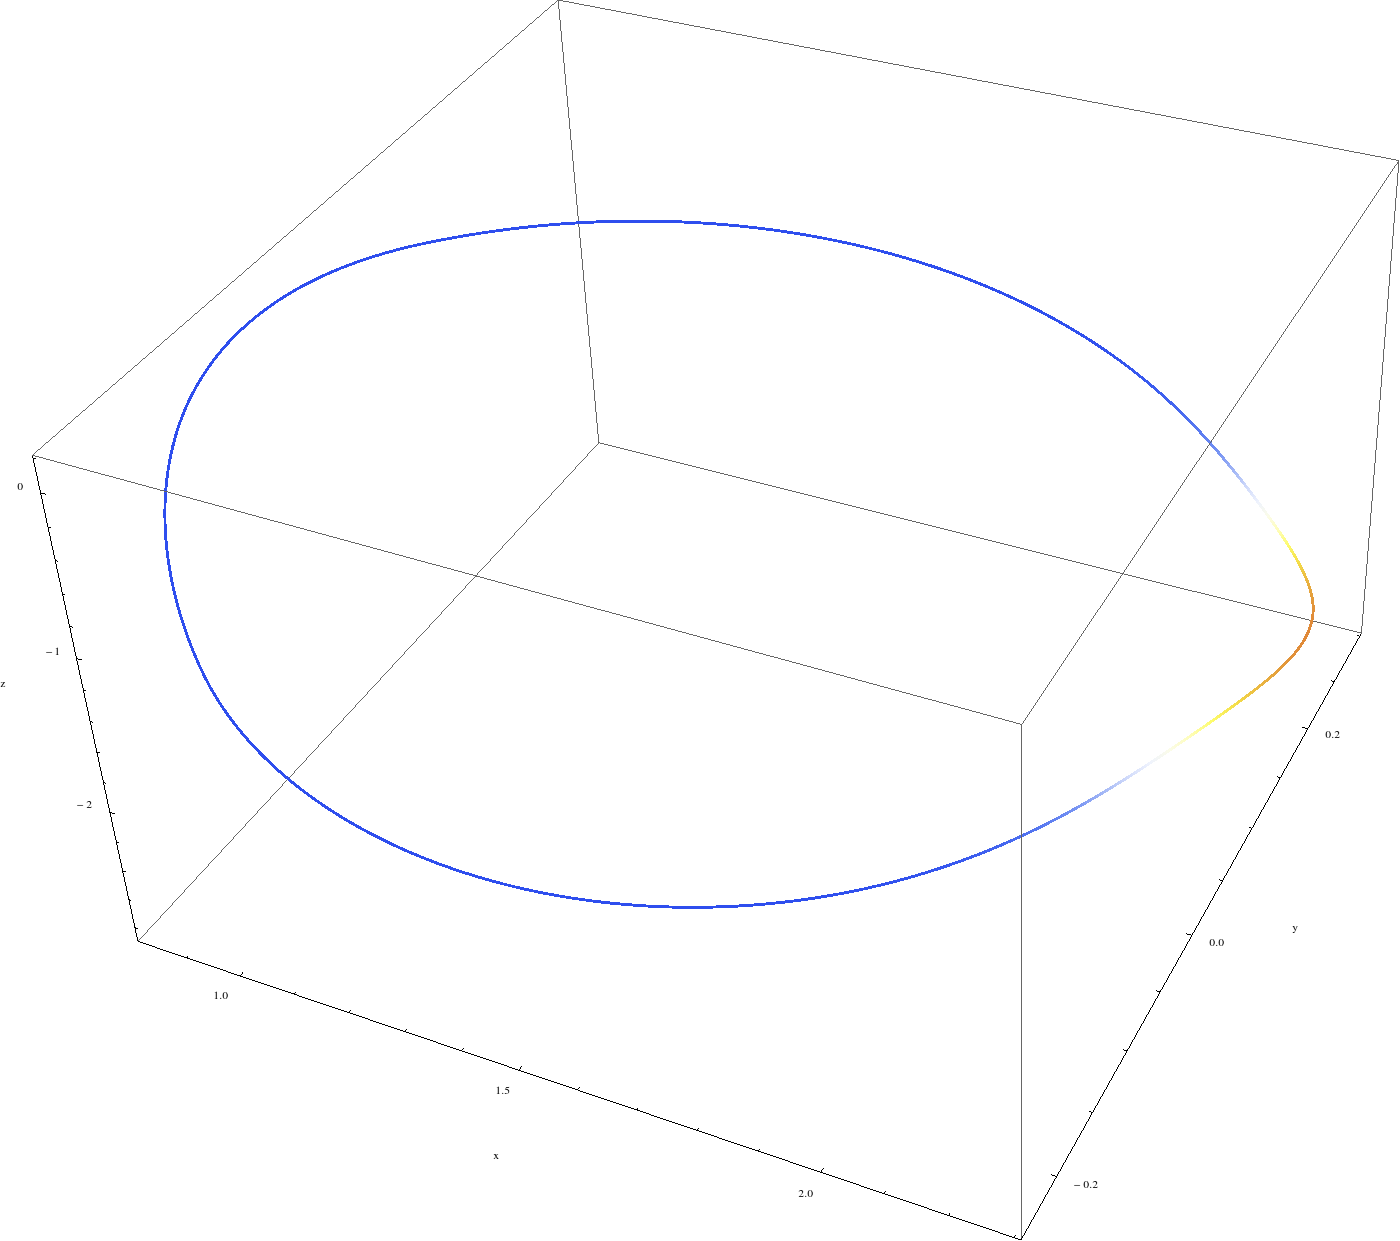
\includegraphics[width=0.45\textheight]{controllers/chua-circuit/Limited-chua-circuit-z-softness-0-13-2-15.png}
\caption[Figure of period 1 limit cycle]{Figures of period 1 limit cycle with one with a fast and one with a slow convergence to the limit cycle. The limit values are \(2.183\) for the upper and \(2.15\) for the lower plots. The convergence to the limit cycle is grayed out so that the final limit cycle's visibility is enhanced.}
\label{figure:z-1-limit-cycle-ctrajectories}
\end{figure}

\begin{figure}[H]
\centering
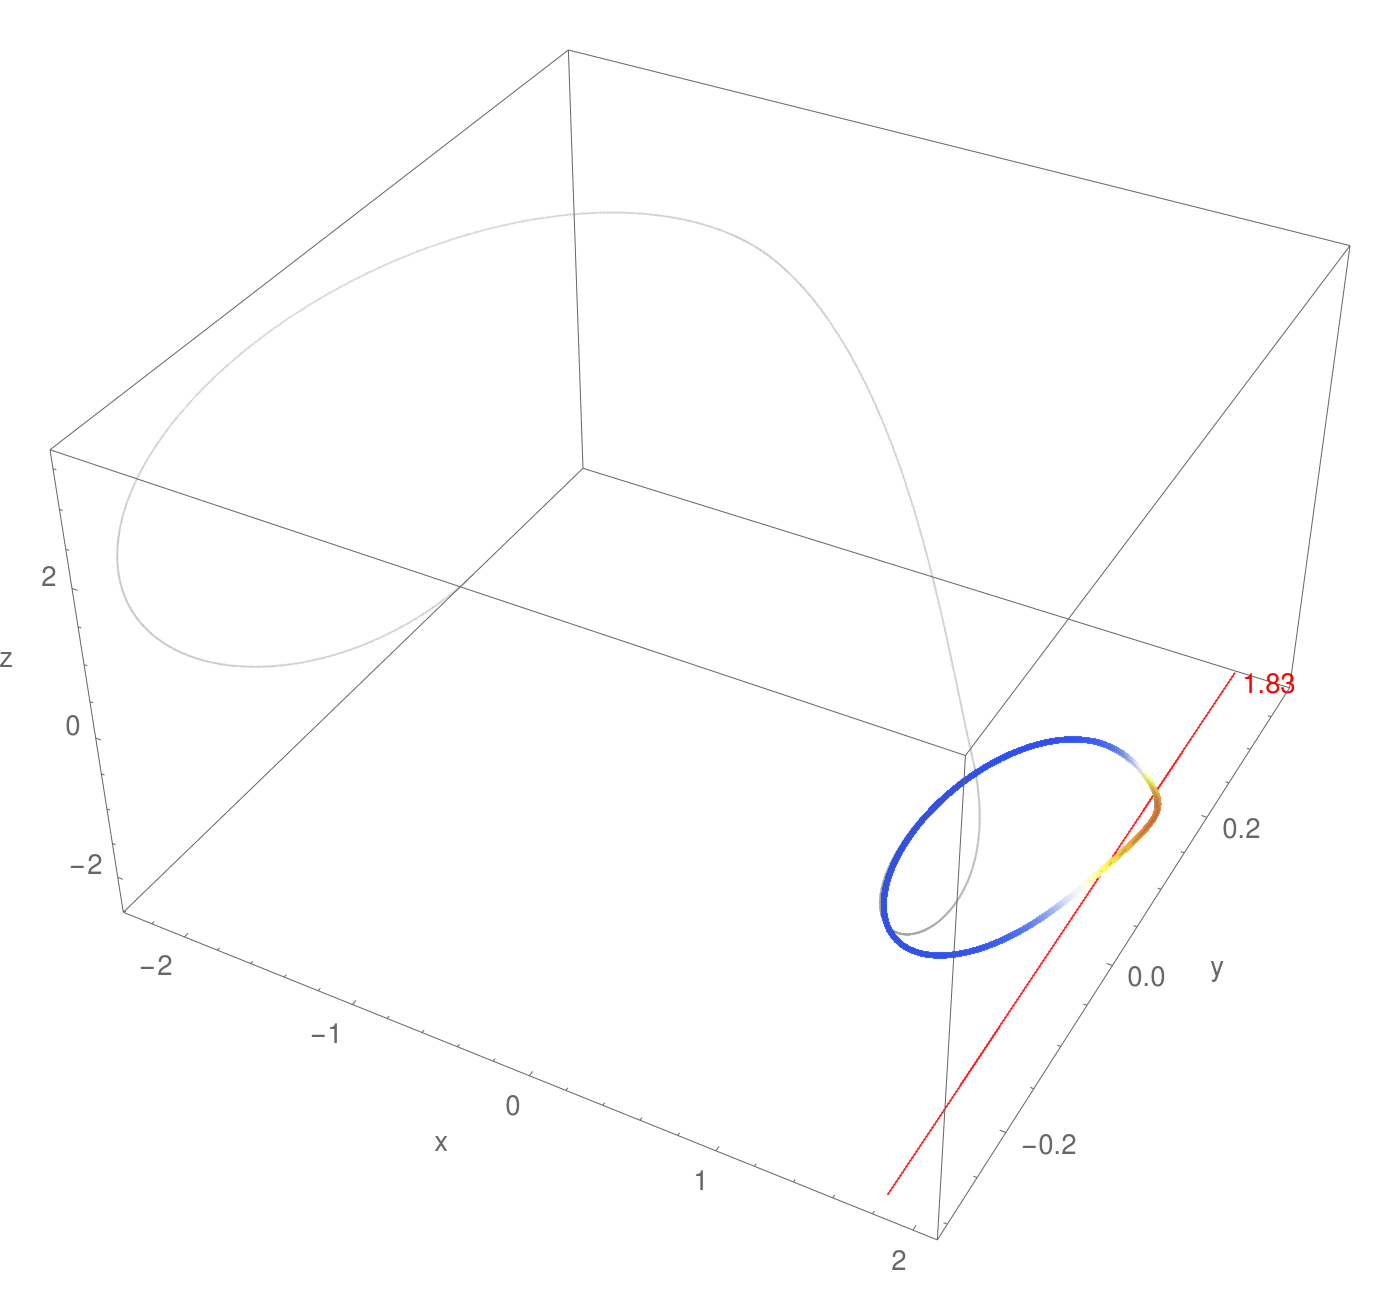
\includegraphics[width=0.45\textheight]{controllers/chua-circuit/Limited-chua-circuit-z-softness-0-13-1-83-convergence.png}
%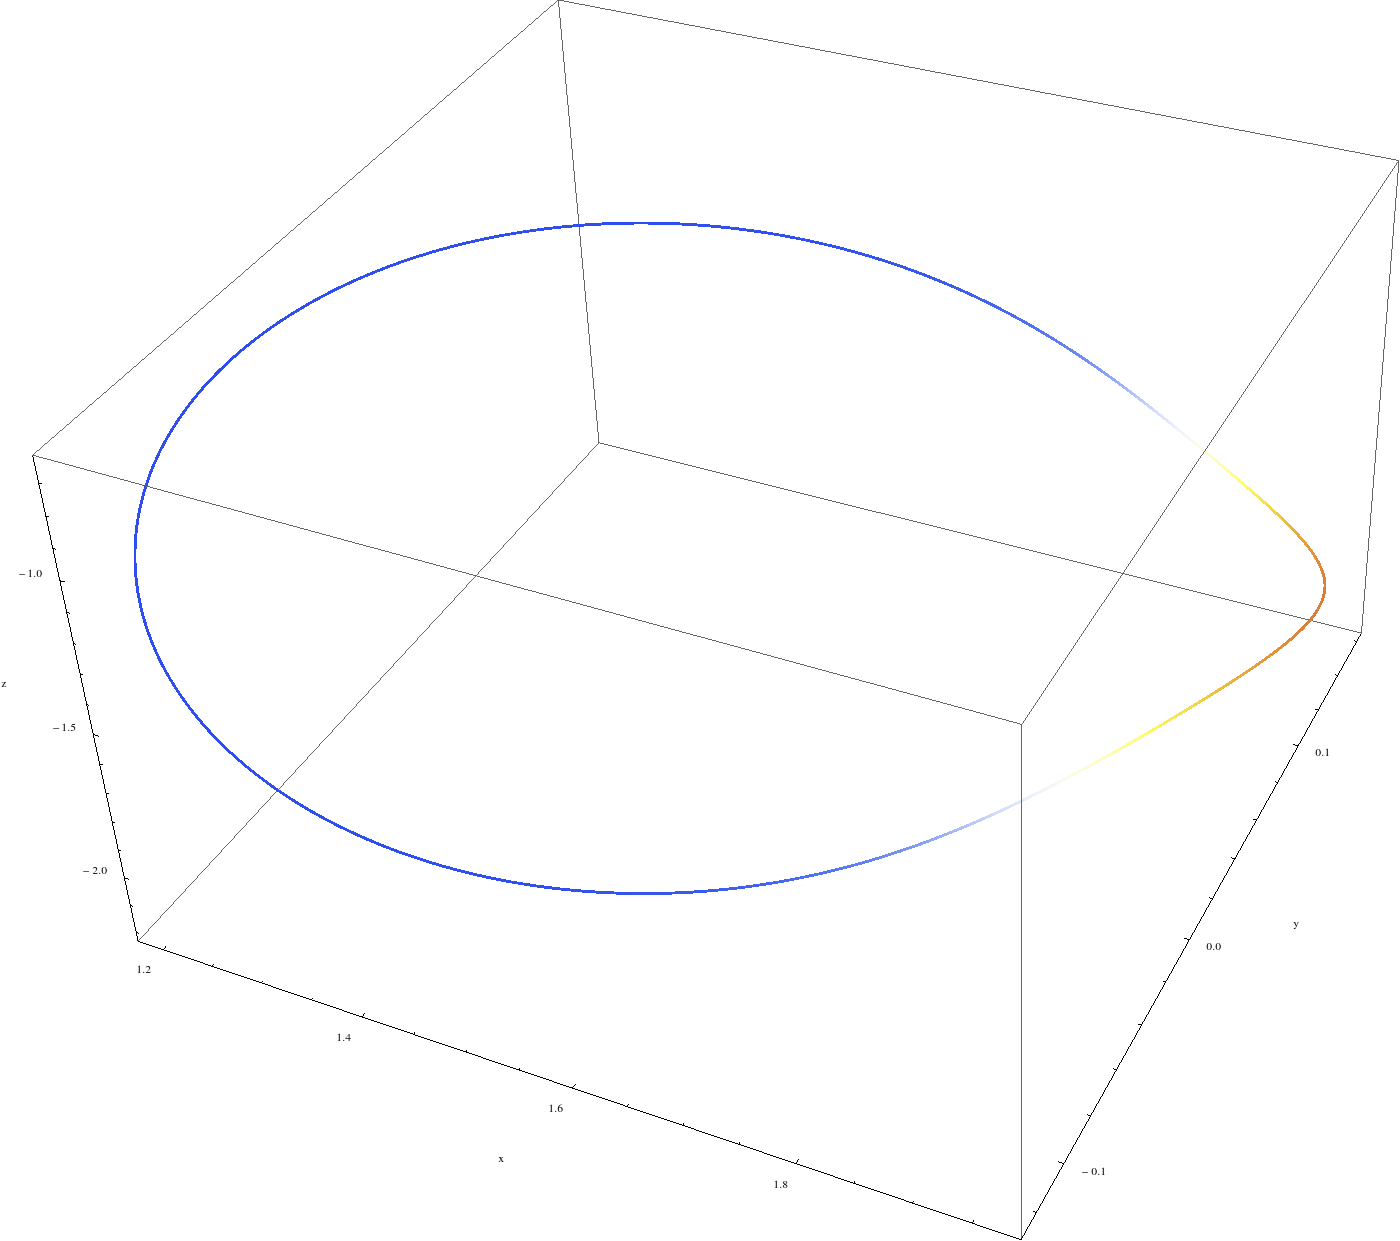
\includegraphics[width=0.45\textheight]{controllers/chua-circuit/Limited-chua-circuit-z-softness-0-13-1-83.png}
\caption[Figure of another period 1 limit cycle]{Figure of period 1 limit cycle with again a fast convergence to the limit cycle using a limit value of \(1.83\). The plot to the right does not show the convergence trajectory, but instead show the periodic orbit after proper convergence.}
\label{figure:z-fast-1-limit-cycle-trajectory}
\end{figure}

Below 1.81, the limiter is applied instantly, the trajectory drops in z direction to \(\approx-2.68343\) and then heads towards \([\infty,\infty,-2.68343]\), therefore can never escape the limiter again.

\todo[inline]{Identify some periodic trajectories, possibly with the help of the group.}

The limiter control gets more interesting when the softness is set to \(softness=0.5\), which corresponds to a softer limiter (Fig. \ref{figure:softlimiterresponse}). %
%
The softer limiter is applied earlier than the hard limiter because of its long tails from the \(\tanh()\) function, however, its influence is rather minimal yet gradually increasing when the limiter is approached. %
%
An extended parameter window for the limiter parameter can now be found, being \(limitValue \in [2.3887,11.5065]\), where the limiter suppresses chaotic behavior and again reduces the number of times the trajectory switches back into the uppermost scroll.

Within the parameter window \(limitValue \in [2.05888,2.387[\), the influence of the limiter keeps the trajectory in the lowermost scroll. %
%
With the softer limiter, it is now much easier to find the parameter window to see the period doubling, because the parameter windows for the different periodicities are now much larger. 

The table \ref{table:z-0.5-periodicities} shows different limit values that stabilize different periodicities.

\begin{table}[H]
\renewcommand{\arraystretch}{1.2}
\center
\begin{tabular}{@{}ll@{}}
	\toprule
   \(limitValue\) & Limit Cycle\\
   \midrule
   2.292 & Period 8 \\ 
   2.285 & Period 4 \\
   2.25  & Period 2 \\
   2.12 & Period 1 \\
   \bottomrule
\end{tabular}
\caption[Periodicity control limit values (x(t) limiting z(t) with softness 0.5)]{Different limit values resulting in trajectories of different periodicity where x(t) limits z(t) using a 0.5 soft limiter.}
\label{table:z-0.5-periodicities}
\end{table}

The plots below show the periodic trajectories for various limit values. The convergence trajectory is grayed out again in the following plots.

\todo[inline]{Could it be that the period doubling is harder to find or doubling is not synchronous anymore?}

\begin{figure}[H]
\centering
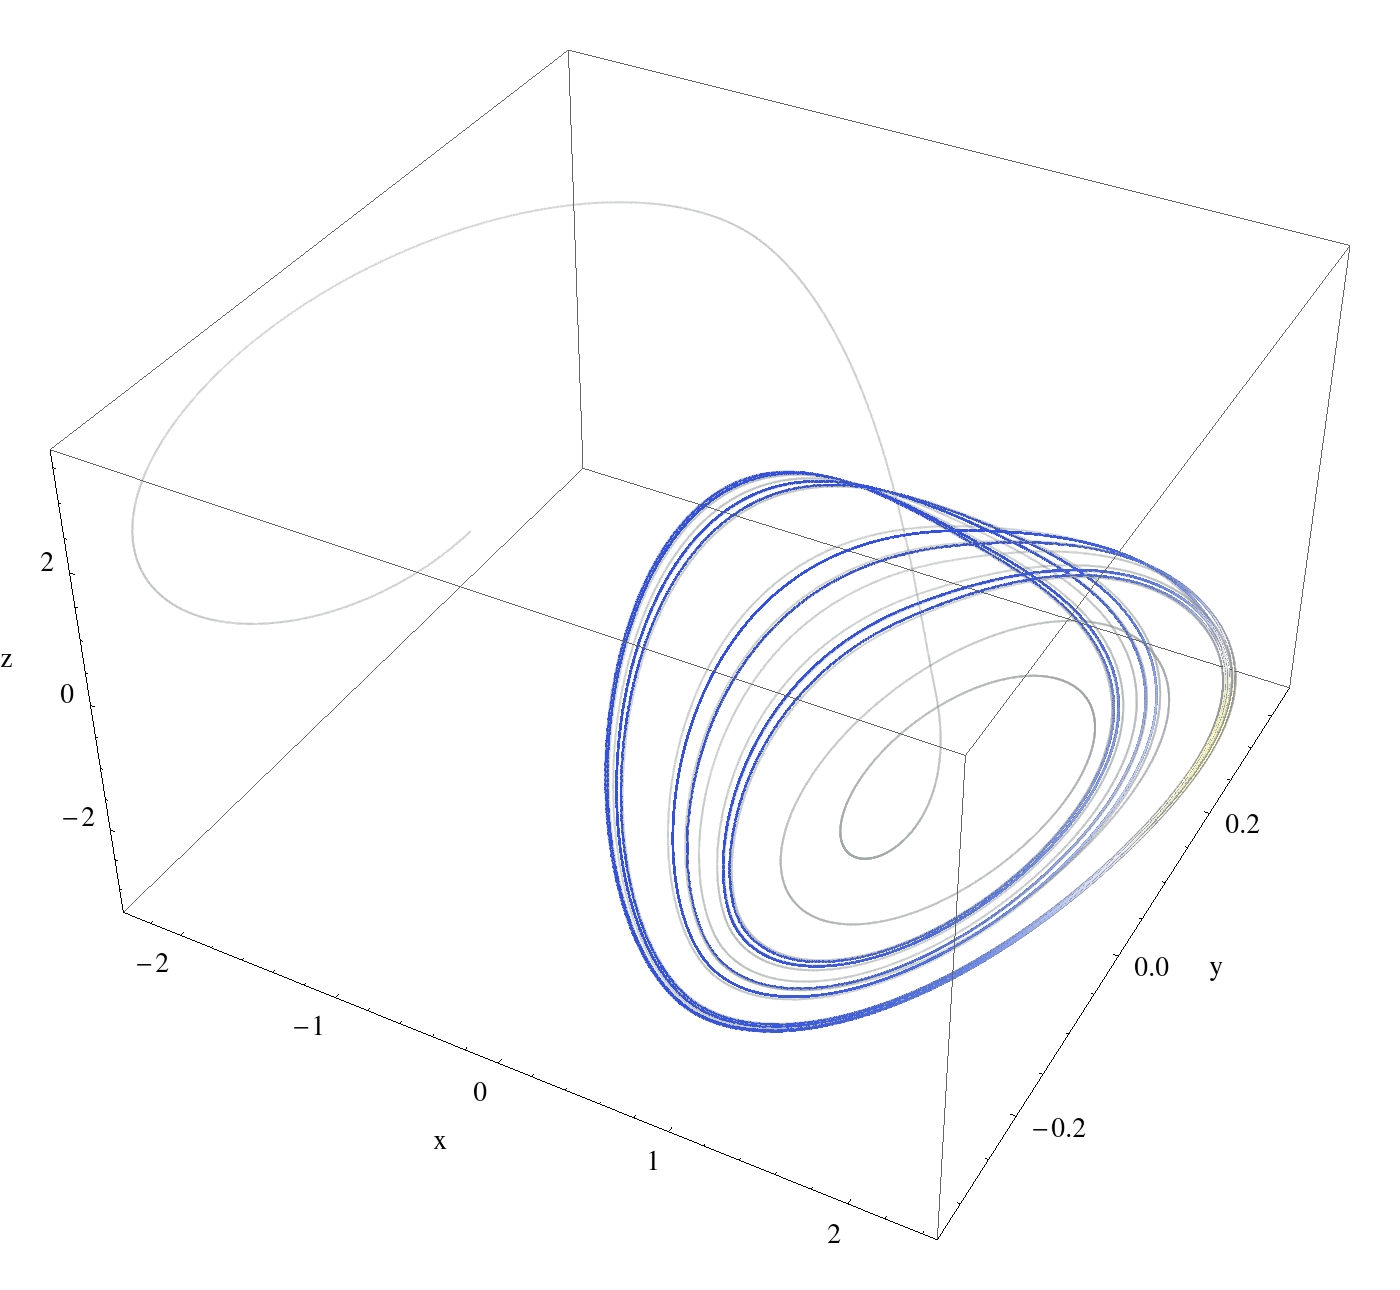
\includegraphics[height=0.45\textheight]{controllers/chua-circuit/Limited-chua-circuit-z-softness-0-5-2-292-convergence.png}
\caption[Figure of period 8 limit cycle using a 0.5 soft limiter.]{Figure of period 8 limit cycle where x(t) limits z(t) using a 0.5 soft limiter.}
\label{figure:z-0.5-8-limit-cycle-trajectory}
\end{figure}

\begin{figure}[H]
\centering
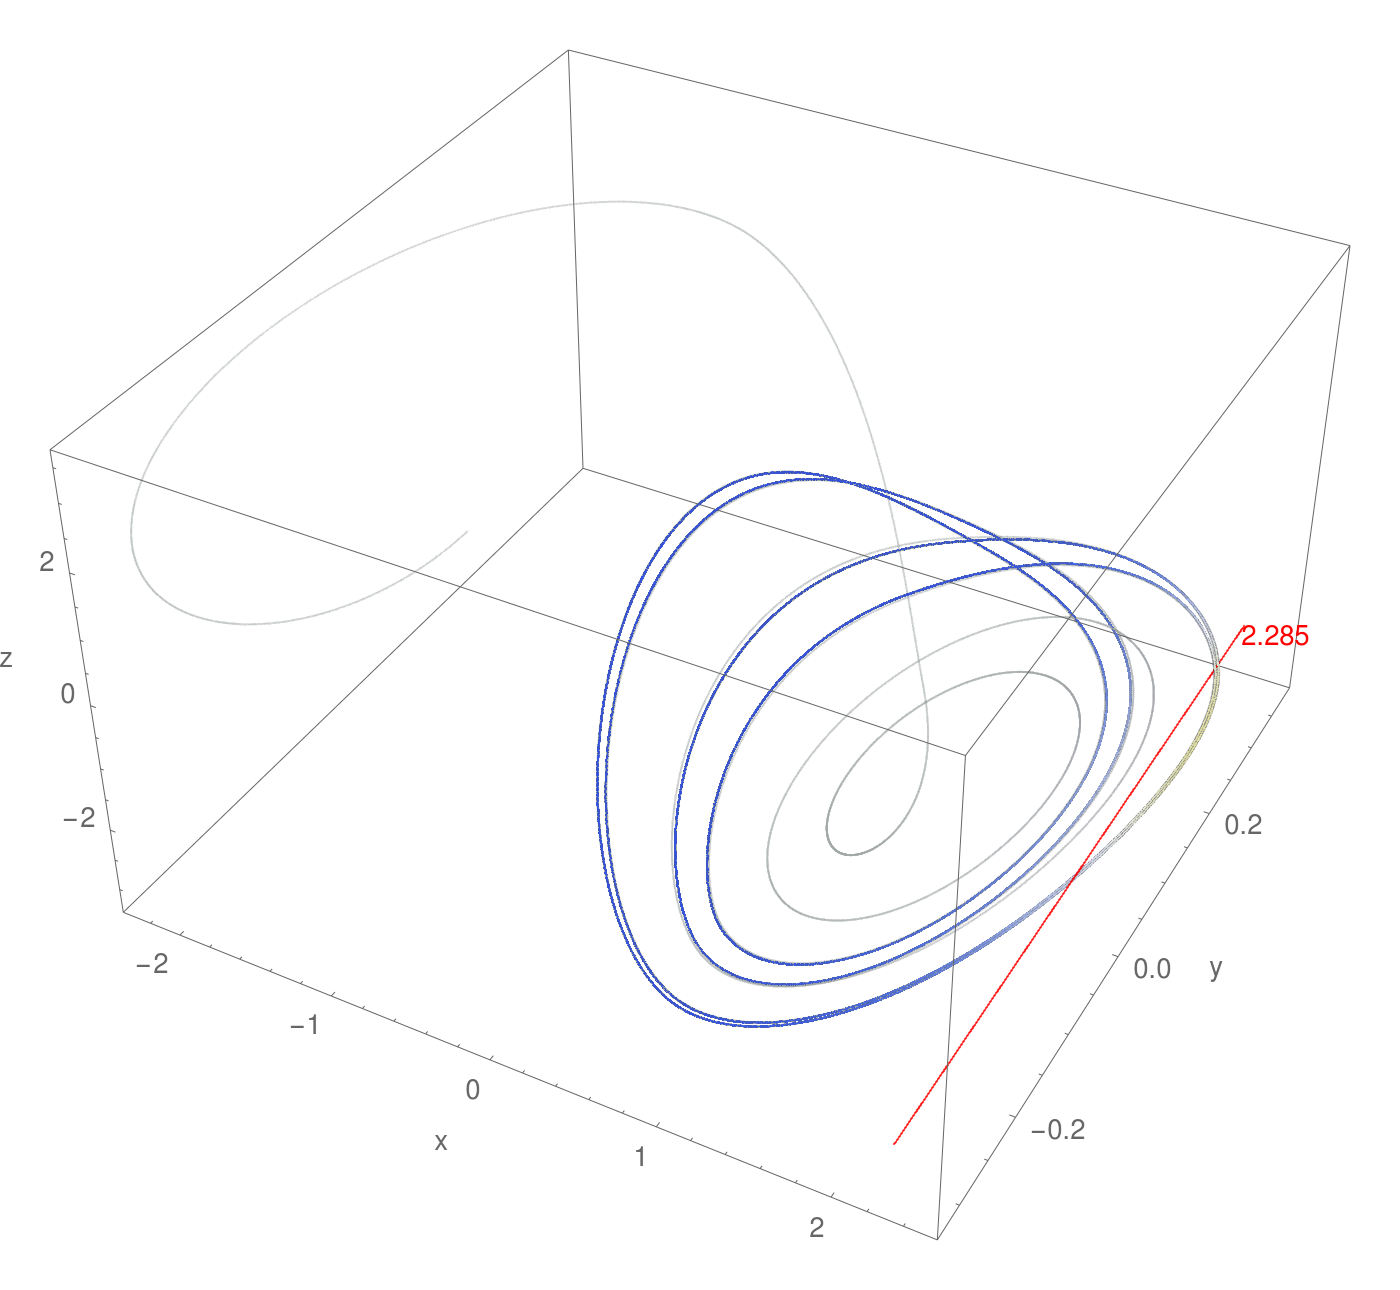
\includegraphics[height=0.45\textheight]{controllers/chua-circuit/Limited-chua-circuit-z-softness-0-5-2-285-convergence.png}
\caption[Figure of period 4 limit cycle using a 0.5 soft limiter.]{Figure of period 4 limit cycle where x(t) limits z(t) using a 0.5 soft limiter.}
\label{figure:z-0.5-4-limit-cycle-trajectory}
\end{figure}

\begin{figure}[H]
\centering
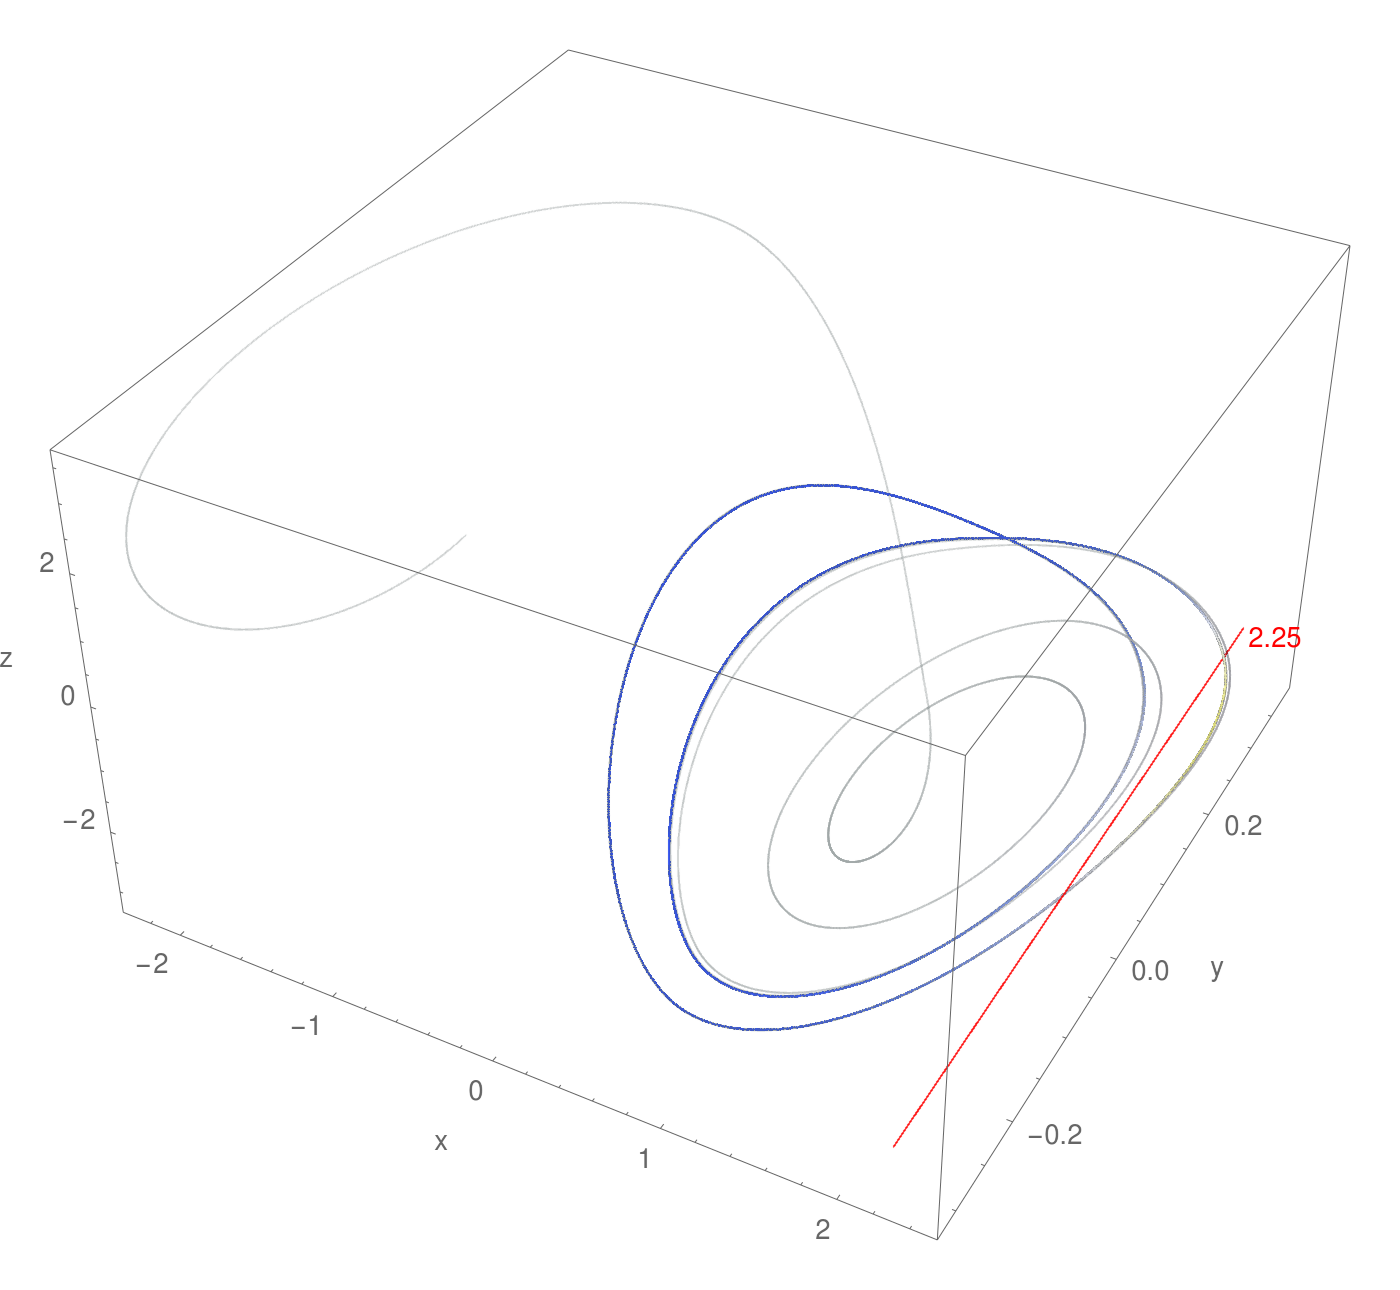
\includegraphics[height=0.45\textheight]{controllers/chua-circuit/Limited-chua-circuit-z-softness-0-5-2-25-convergence.png}
\caption[Figure of period 2 limit cycle using a 0.5 soft limiter.]{Figure of period 2 limit cycle where x(t) limits z(t) using a 0.5 soft limiter.}
\label{figure:z-0.5-2-limit-cycle-trajectory}
\end{figure}

\begin{figure}[H]
\centering
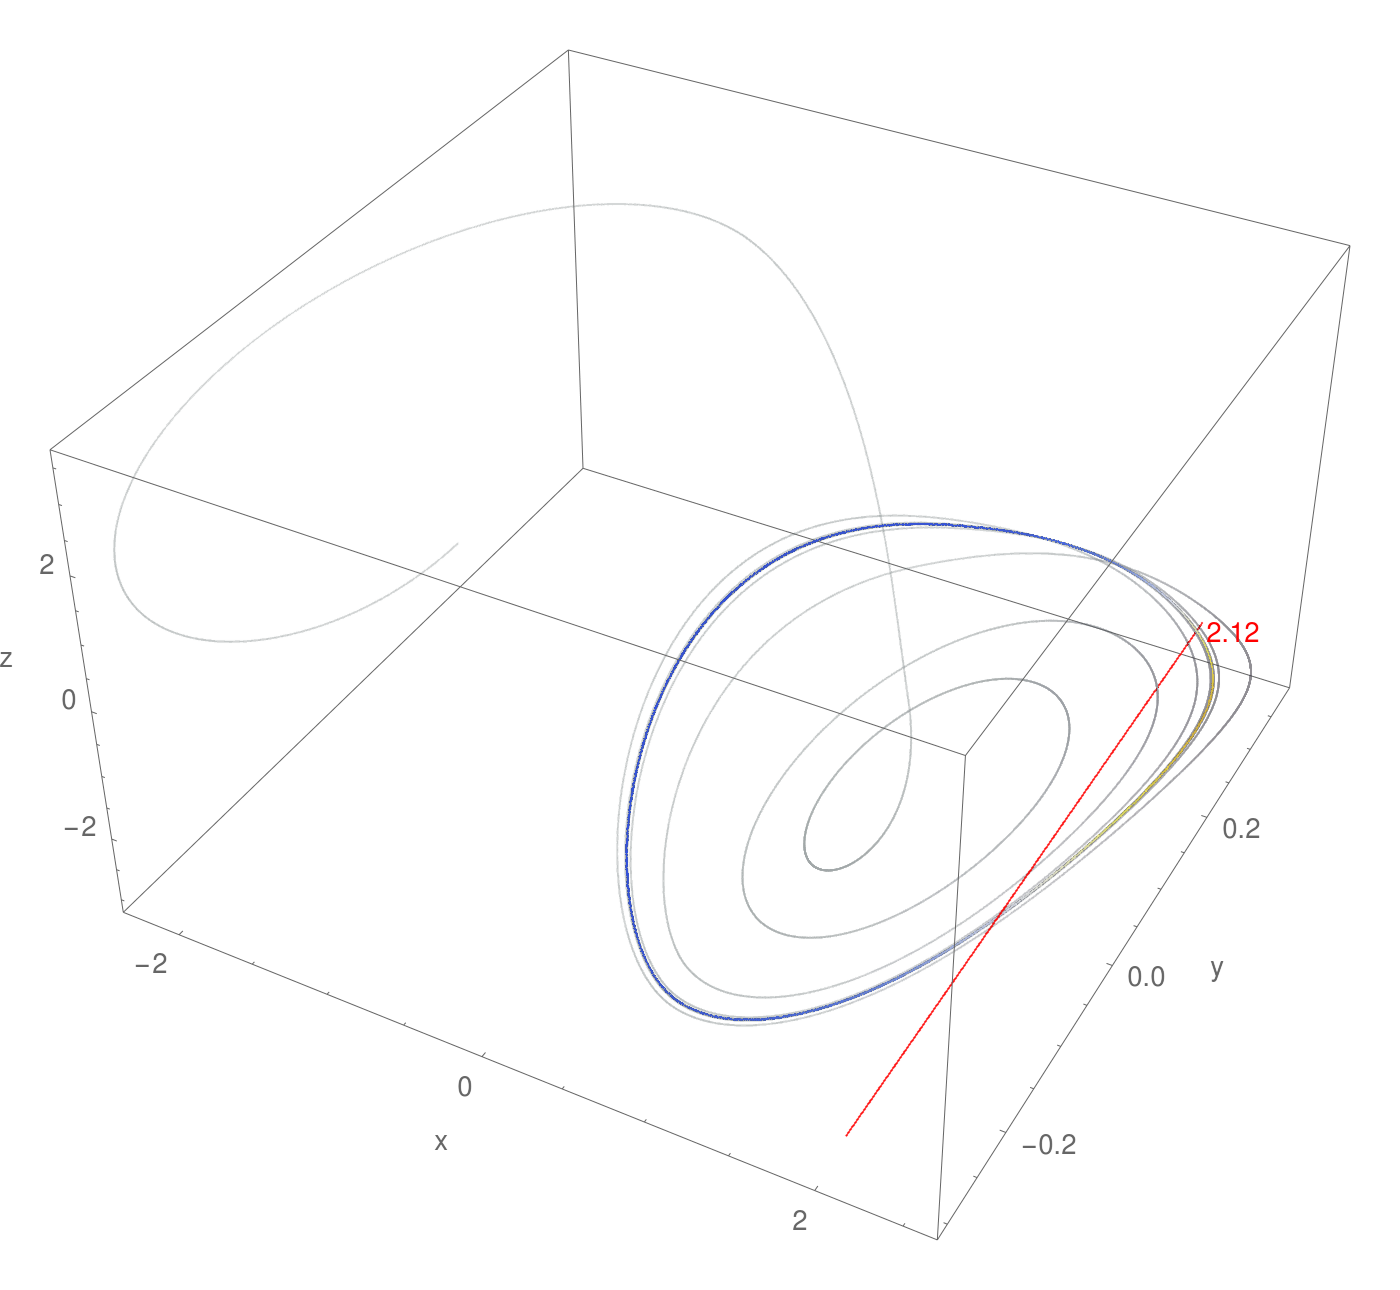
\includegraphics[height=0.45\textheight]{controllers/chua-circuit/Limited-chua-circuit-z-softness-0-5-2-12-convergence.png}
\caption[Figure of period 1 limit cycle using a 0.5 soft limiter.]{Figure of period 1 limit cycle where x(t) limits z(t) using a 0.5 soft limiter.}
\label{figure:z-0.5-1-limit-cycle-trajectory}
\end{figure}

\paragraph{One Dimension Limiting Itself} In the second experiment, the softnss is again set to \(softness=0.13\) to approximate a rather hard limiter. The limiter is added to the equations as shown below:

\begin{align*}
\frac{dx}{dt}&=\alpha (y-x-f(x)) ~ \text{softLim}(x)\\
\frac{dy}{dt}&=\beta (x-y + Rz)\\
\frac{dz}{dt}&=-\gamma ~ y\\
f (x) &= \frac{m_1 x + (m_0 - m_1)}{2 (| x + E | -| x - E |)}
\end{align*}

If the $limitValue$ parameter is changed from \(>4.6692\), which corresponds to no limiter influence to the trajectory, to a value within \(limitValue \in [1.99545,4.6692[\), one can observe different chaotic trajectories. The limiter influences the circuit by limiting the voltage across the capacitor \(C_1\) when \(x\) approaches the limiter. %
%
Within the window \([1.89,1.99545]\) a small limiter parameter window can be found which controls trajectories of high periodicity down to different lower periods. %
%
Period doubling behavior can be found when controlling the Chua circuit appropriately with limit values as described in the table \ref{table:x-0.13-periodicities}.

\begin{table}[H]
\renewcommand{\arraystretch}{1.2}
\center
\begin{tabular}{@{}ll@{}}
	\toprule
   \(limitValue\) & Limit Cycle\\
   \midrule
   1.932 & Period 8 \\ 
   1.93 & Period 4 \\
   1.91  & Period 2 \\
   1.89 & Period 1 \\
   \bottomrule
\end{tabular}
\caption[Limiter values for periodic trajectories for for an x self-limiting limiter with softness 0.13]{Different limit values resulting in trajectories of different periodicity, where x(t) limits itself using a 0.13 soft limiter.}
\label{table:x-0.13-periodicities}
\end{table}

\begin{figure}[H]
\centering
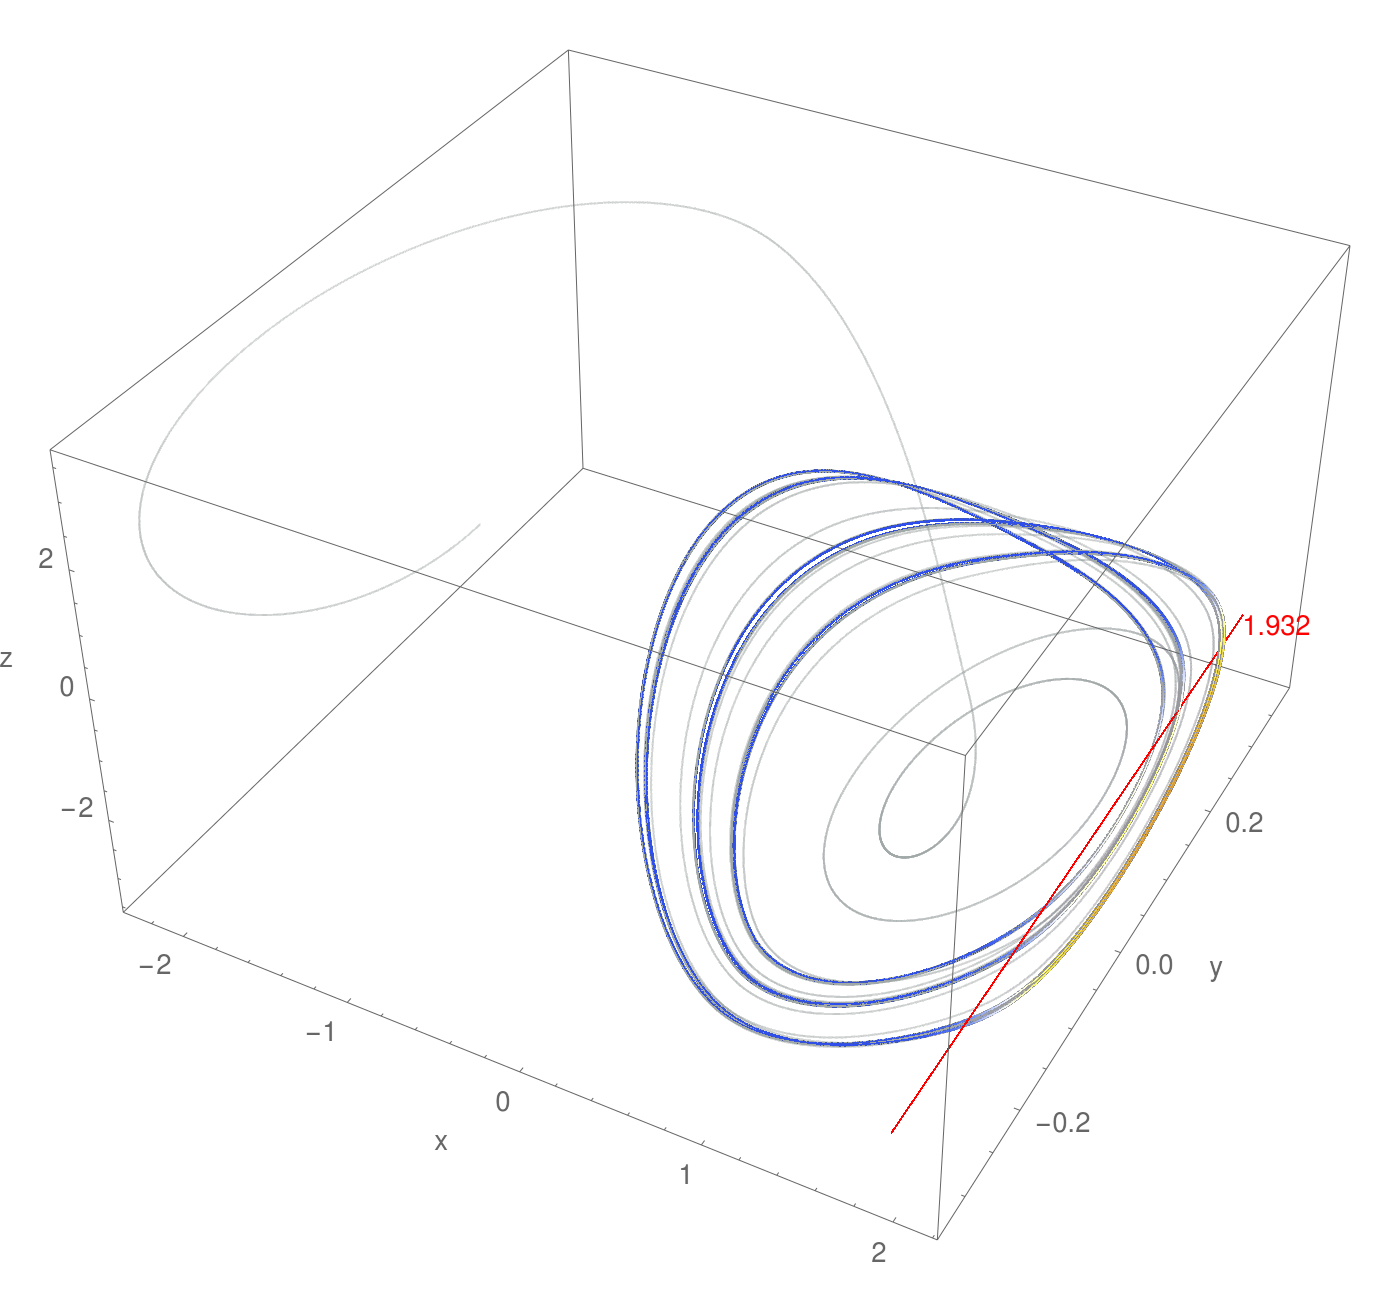
\includegraphics[height=0.45\textheight]{controllers/chua-circuit/Limited-chua-circuit-x-softness-0-13-1-932-convergence.png}
\caption[Figure of period 8 limit cycle using self limiting 0.13 soft limiter]{Figure of period 8 limit cycle when using a self limiter with value 0.13.}
\label{figure:x-0.13-8-limit-cycle-trajectory}
\end{figure}

\begin{figure}[H]
\centering
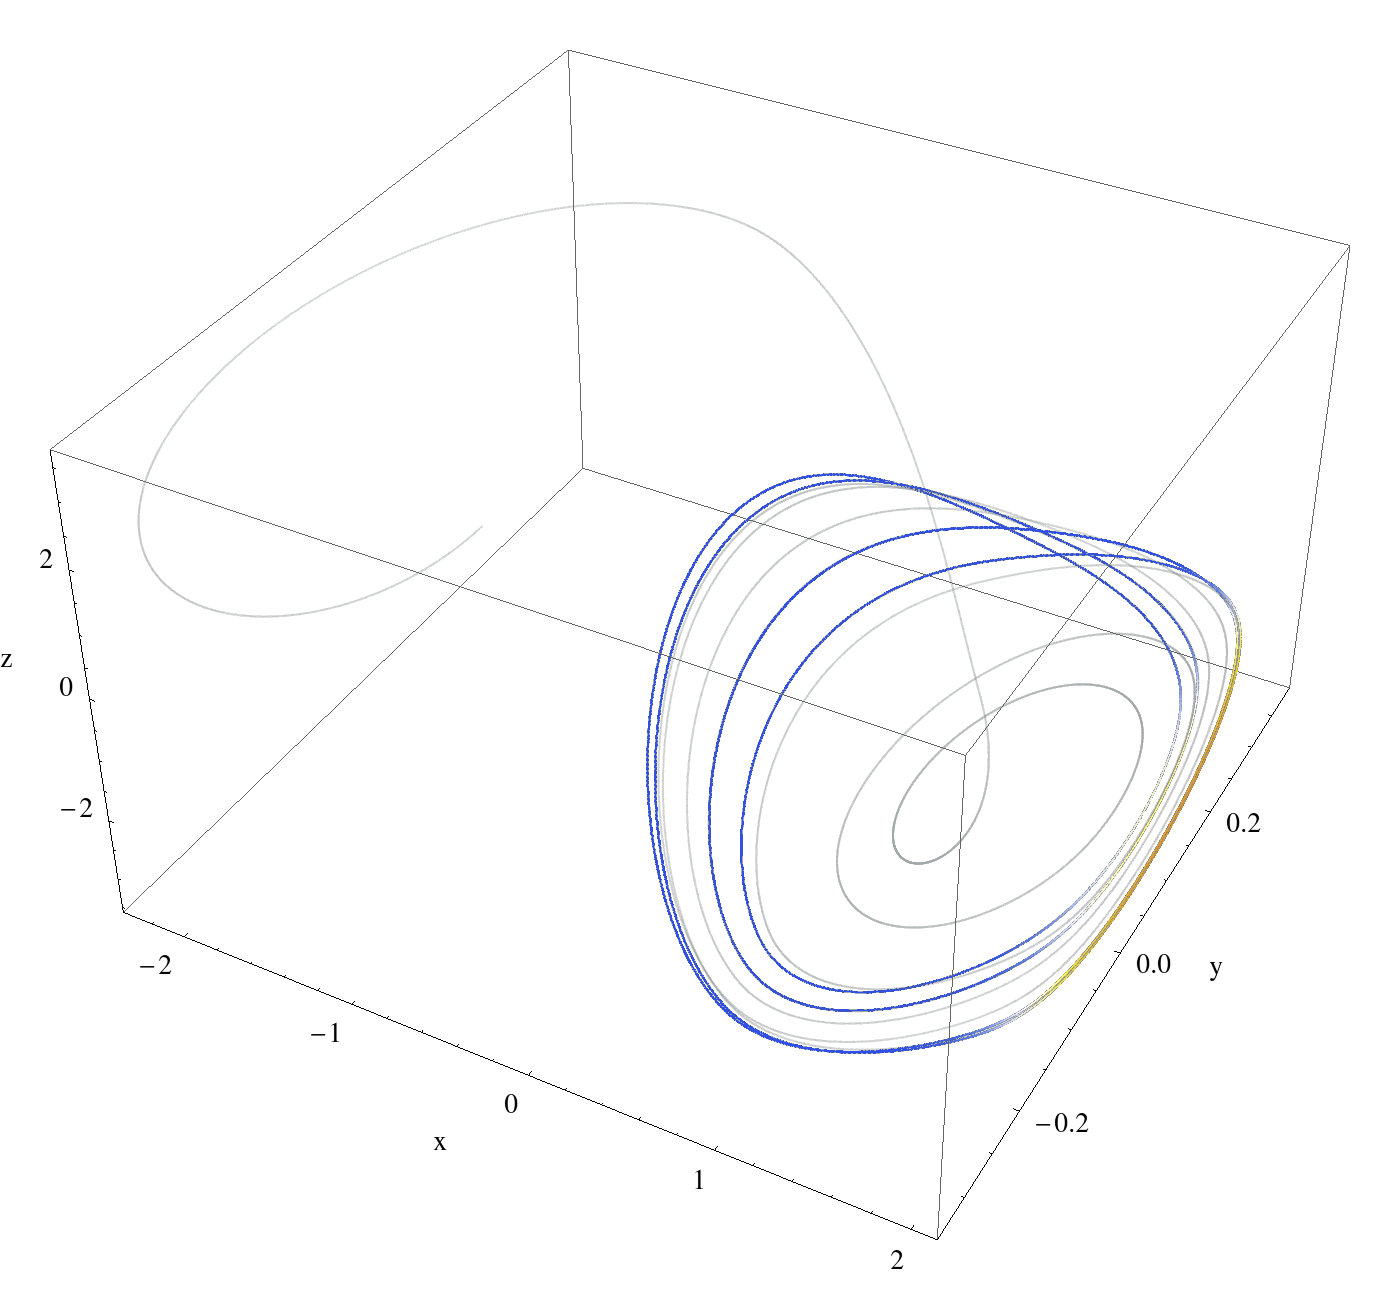
\includegraphics[height=0.45\textheight]{controllers/chua-circuit/Limited-chua-circuit-x-softness-0-13-1-93-convergence.png}
\caption[Figure of period 4 limit cycle using self limiter 0.13 soft limiter]{Figure of period 4 limit cycle when using a self limiter with value 0.13.}
\label{figure:x-0.13-4-limit-cycle-trajectory}
\end{figure}

\begin{figure}[H]
\centering
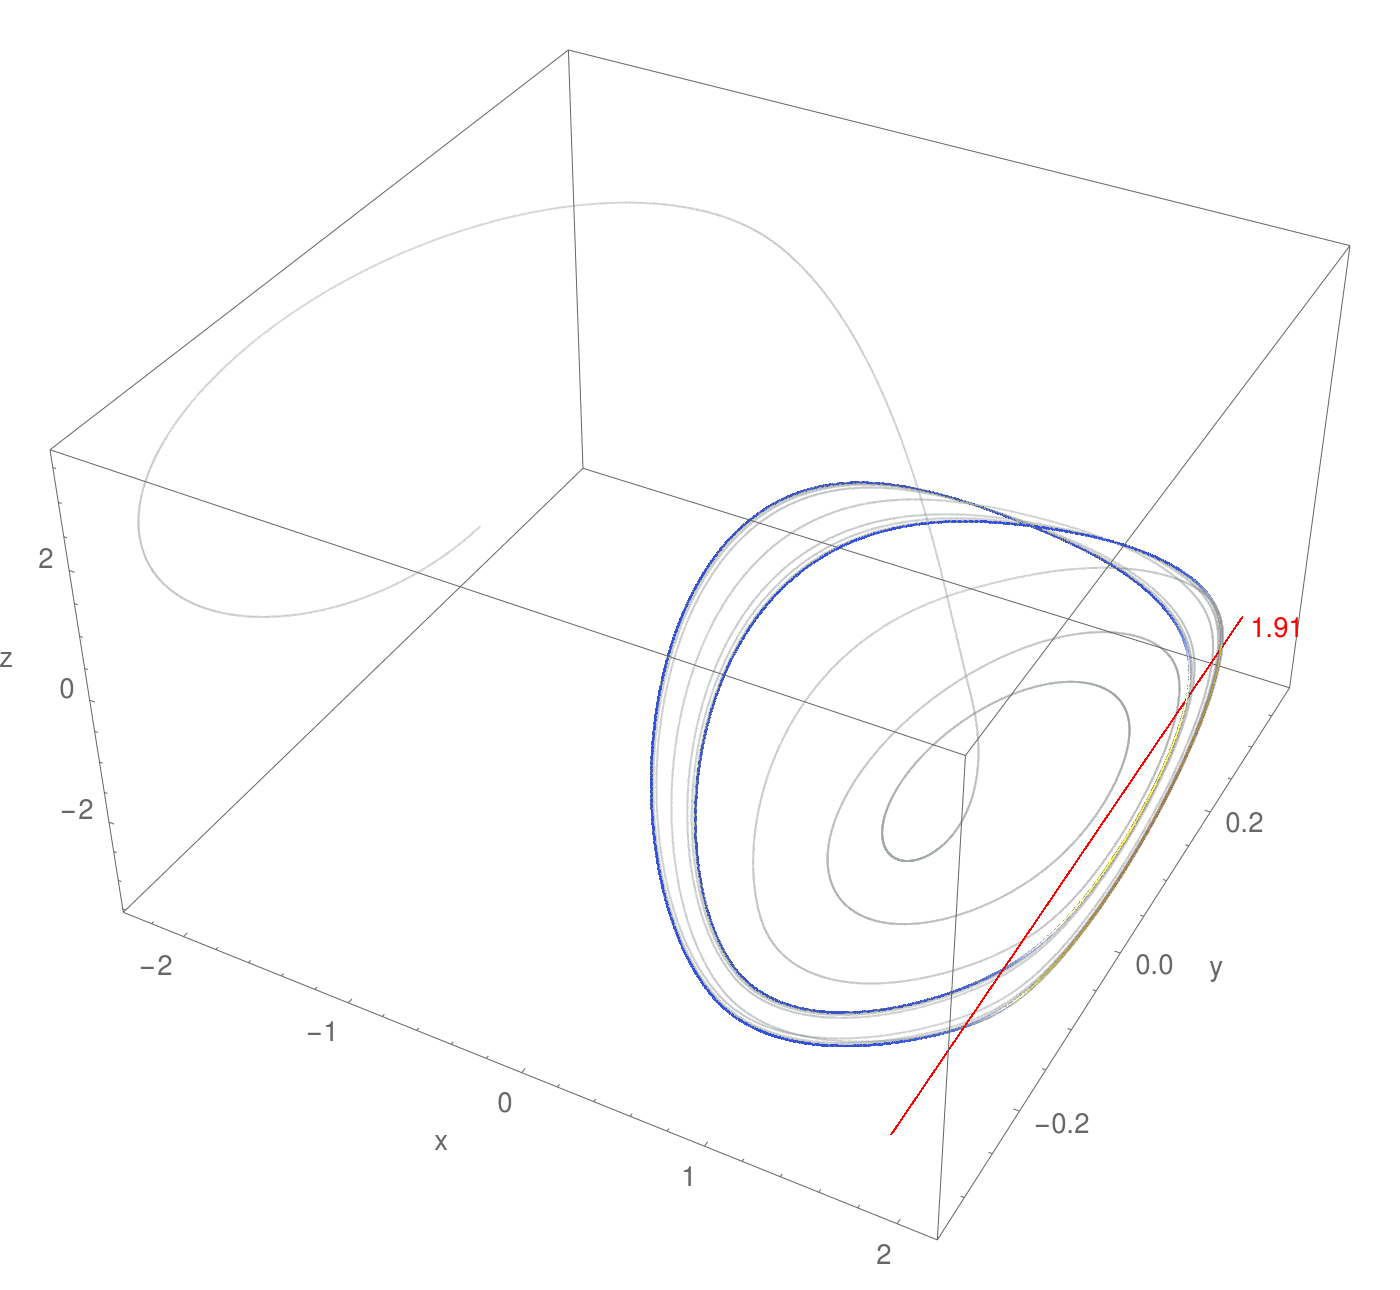
\includegraphics[height=0.45\textheight]{controllers/chua-circuit/Limited-chua-circuit-x-softness-0-13-1-91-convergence.png}
\caption[Figure of period 2 limit cycle using self limiter 0.13 soft limiter]{Figure of period 2 limit cycle when using a self limiter with value 0.13.}
\label{figure:x-0.13-2-limit-cycle-trajectory}
\end{figure}

\begin{figure}[H]
\centering
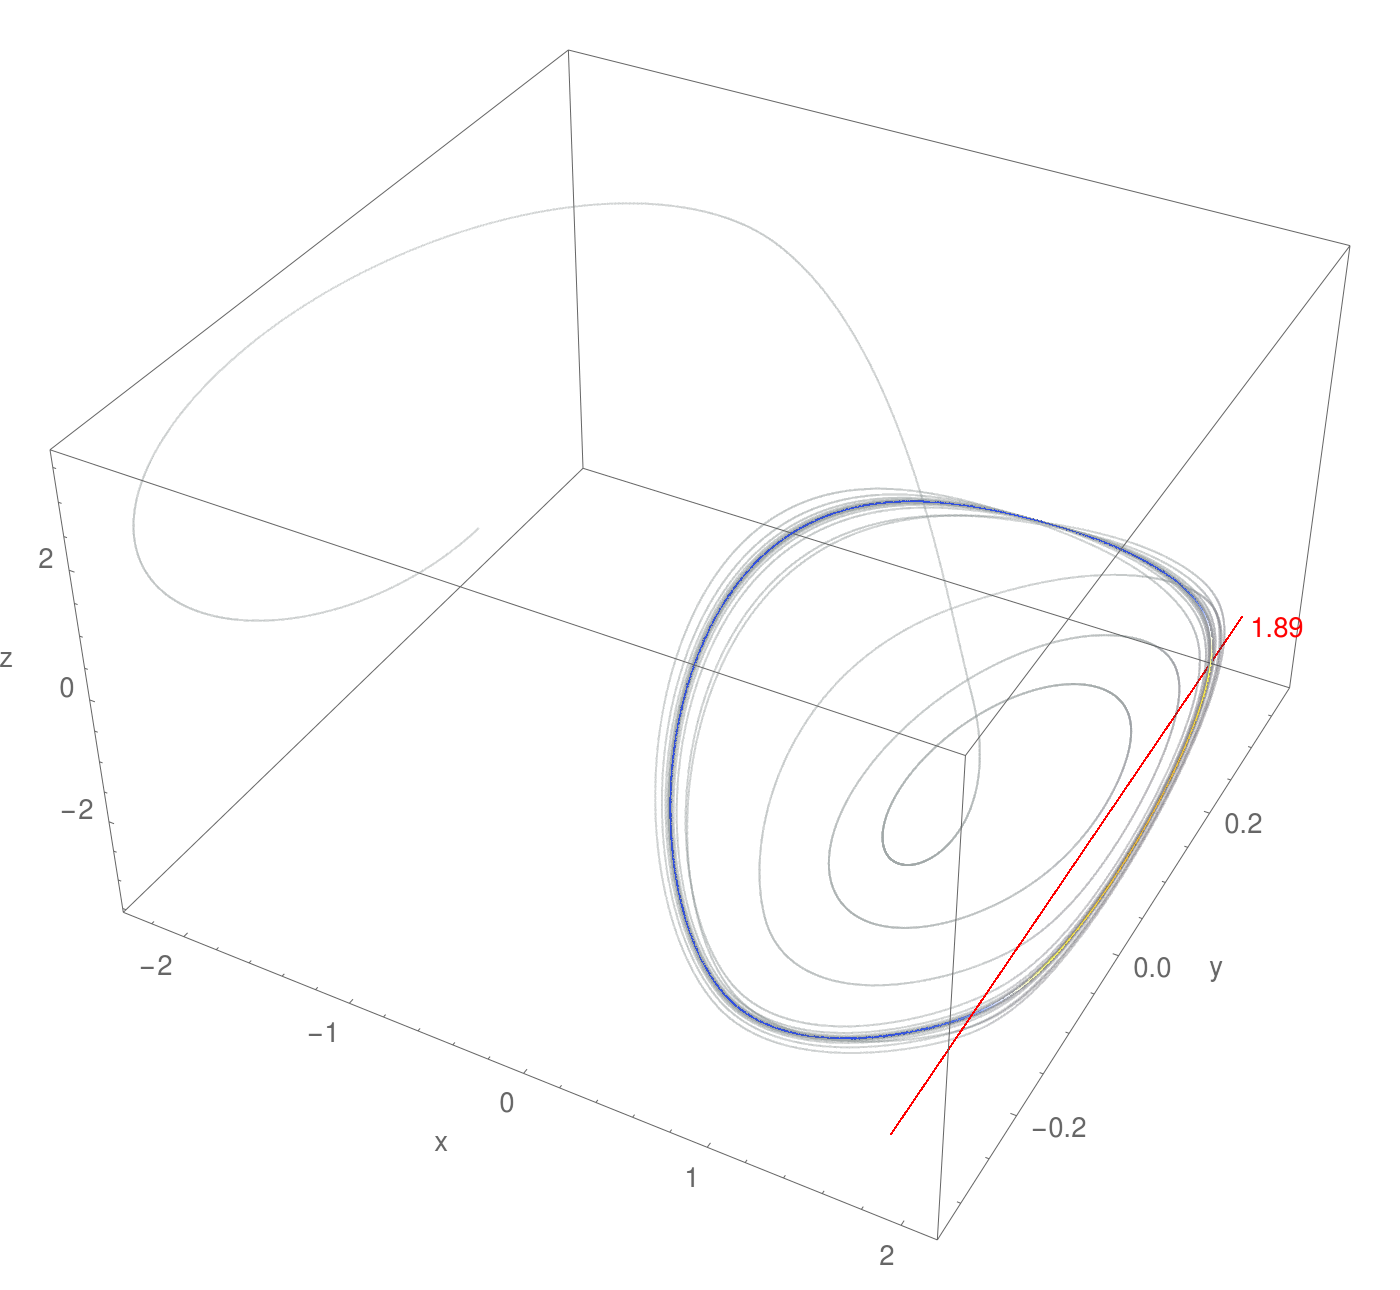
\includegraphics[height=0.45\textheight]{controllers/chua-circuit/Limited-chua-circuit-x-softness-0-13-1-89-convergence.png}
\caption[Figure of period 1 limit cycle using self limiter 0.13 soft limiter]{Figure of period 1 limit cycle when using a self limiter with value 0.13.}
\label{figure:x-0.13-1-limit-cycle-trajectory}
\end{figure}

The hard limiter leads to a very slow convergence and therefore it is hard to determine the final periodicity because every evaluation takes a lot of time. %
%
However, with x limiting itself, the limiter parameter of the system can now be set far beyond the fixed point of the lowermost scroll without the trajectory getting trapped. %
%
At \(limitValue=1.61\), one can observe perfect convergence to period 1.

\begin{figure}[H]
\centering
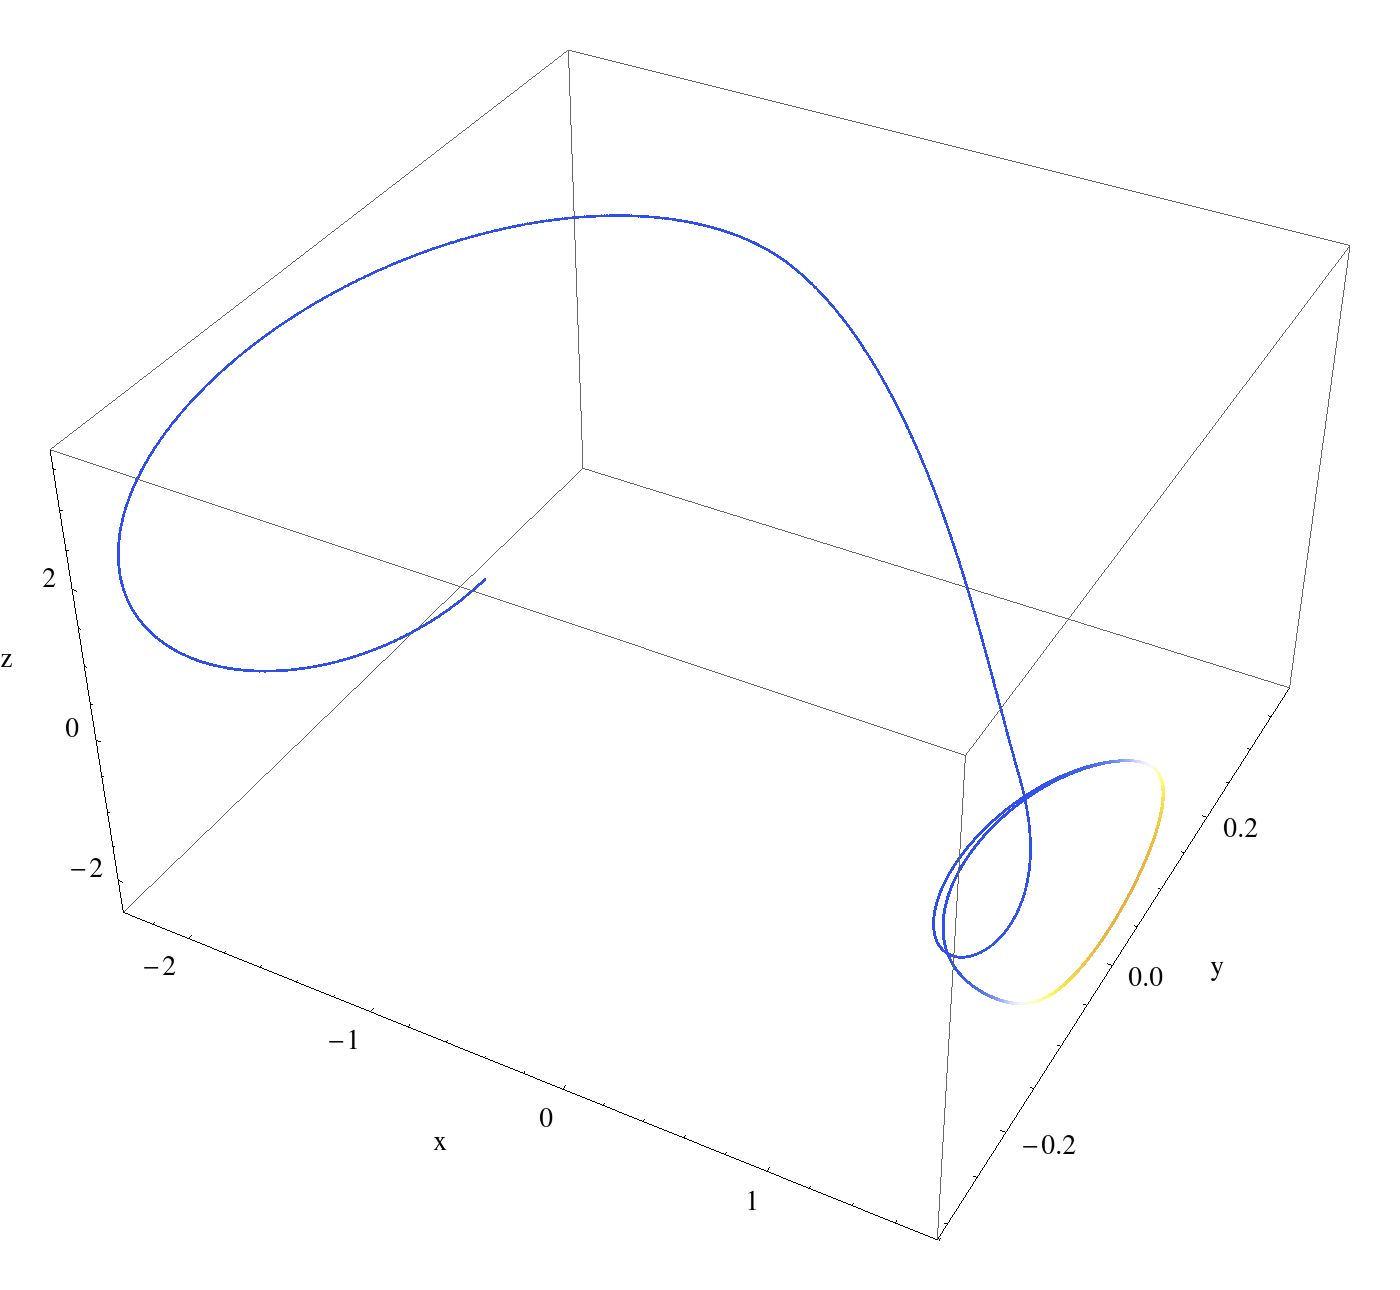
\includegraphics[width=0.8\textwidth]{controllers/chua-circuit/Limited-chua-circuit-x-softness-0-13-1-61-convergence.png}
\caption[Figure of period 1 limit cycle]{Figure of period 1 limit cycle at 1.61.}
\label{figure:x-0.13-fast-1-limit-cycle-trajectory-1-61}
\end{figure}

Surpassing this point increases the convergence time again because the trajectory converges to the limit cycle from outside.

\begin{figure}[H]
\centering
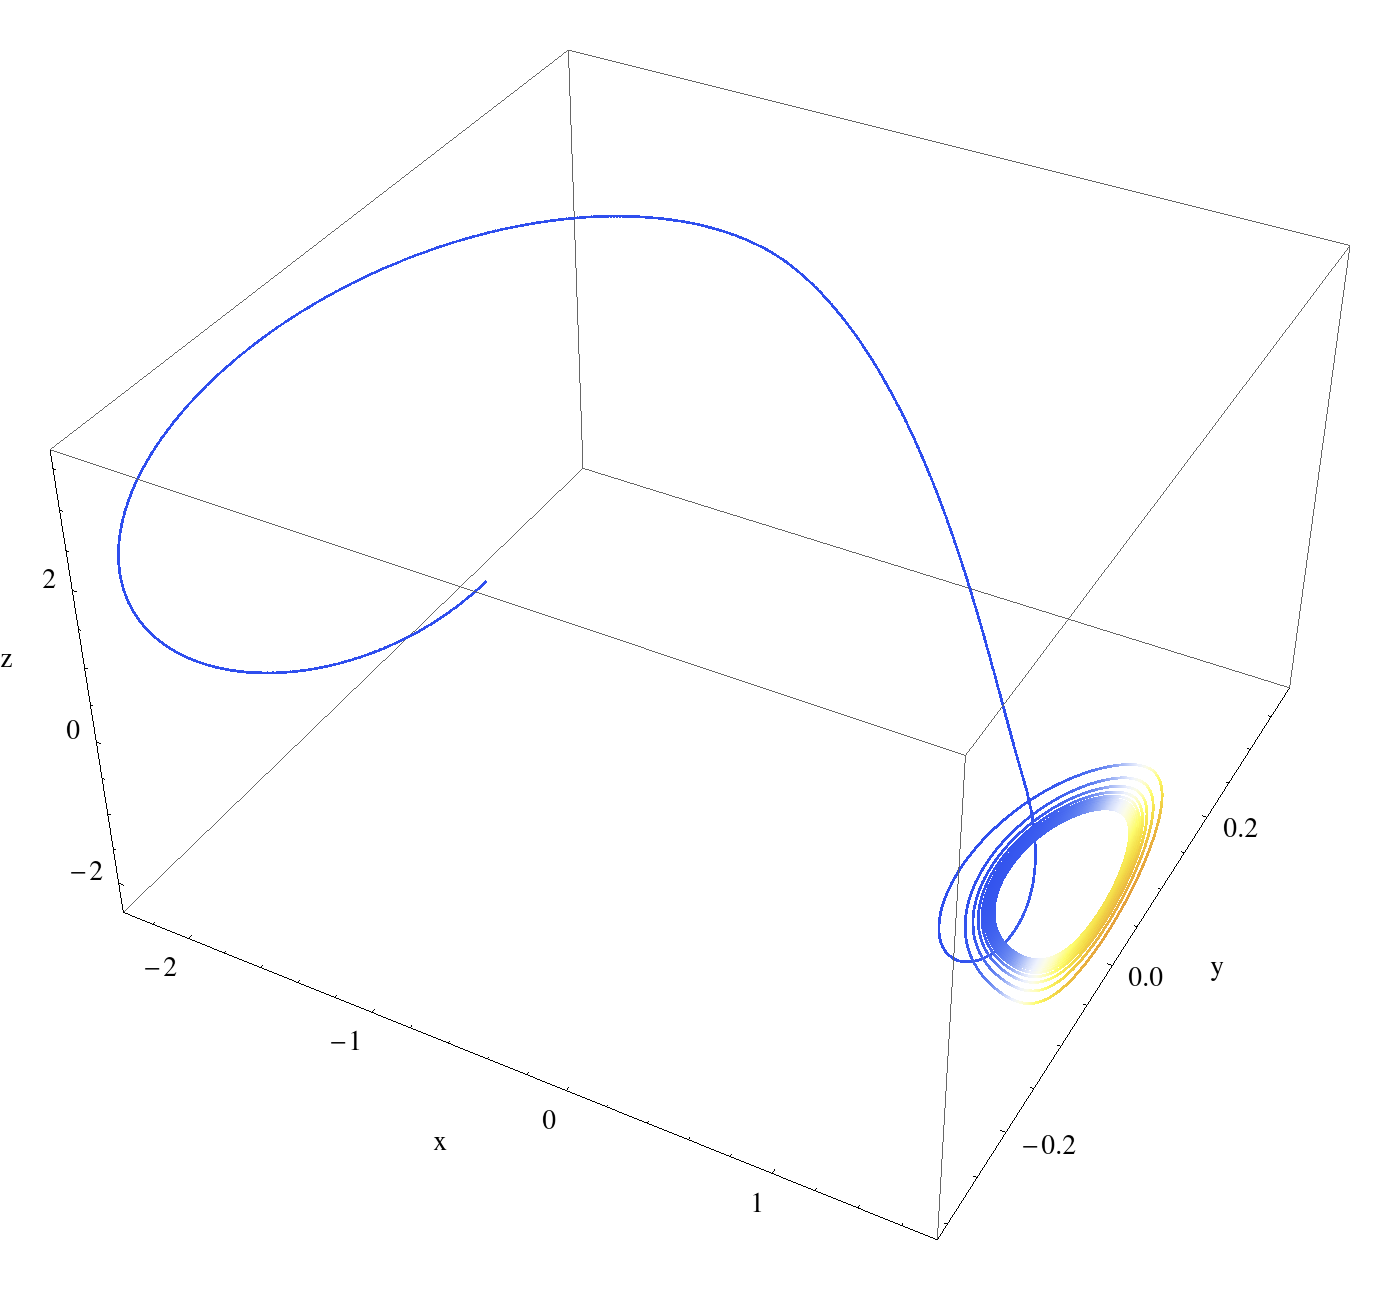
\includegraphics[width=0.8\textwidth]{controllers/chua-circuit/Limited-chua-circuit-x-softness-0-13-1-57-convergence.png}
\caption[Figure of period another 1 limit cycle]{Figure of period 1 limit cycle at 1.57.}
\label{figure:x-0.13-fast-1-limit-cycle-trajectory-1-57}
\end{figure}

The controlled limit cycle shrinks, until the trajectory directly converges onto one single fix point at \(limitValue=1.4\). 

\begin{figure}[H]
\centering
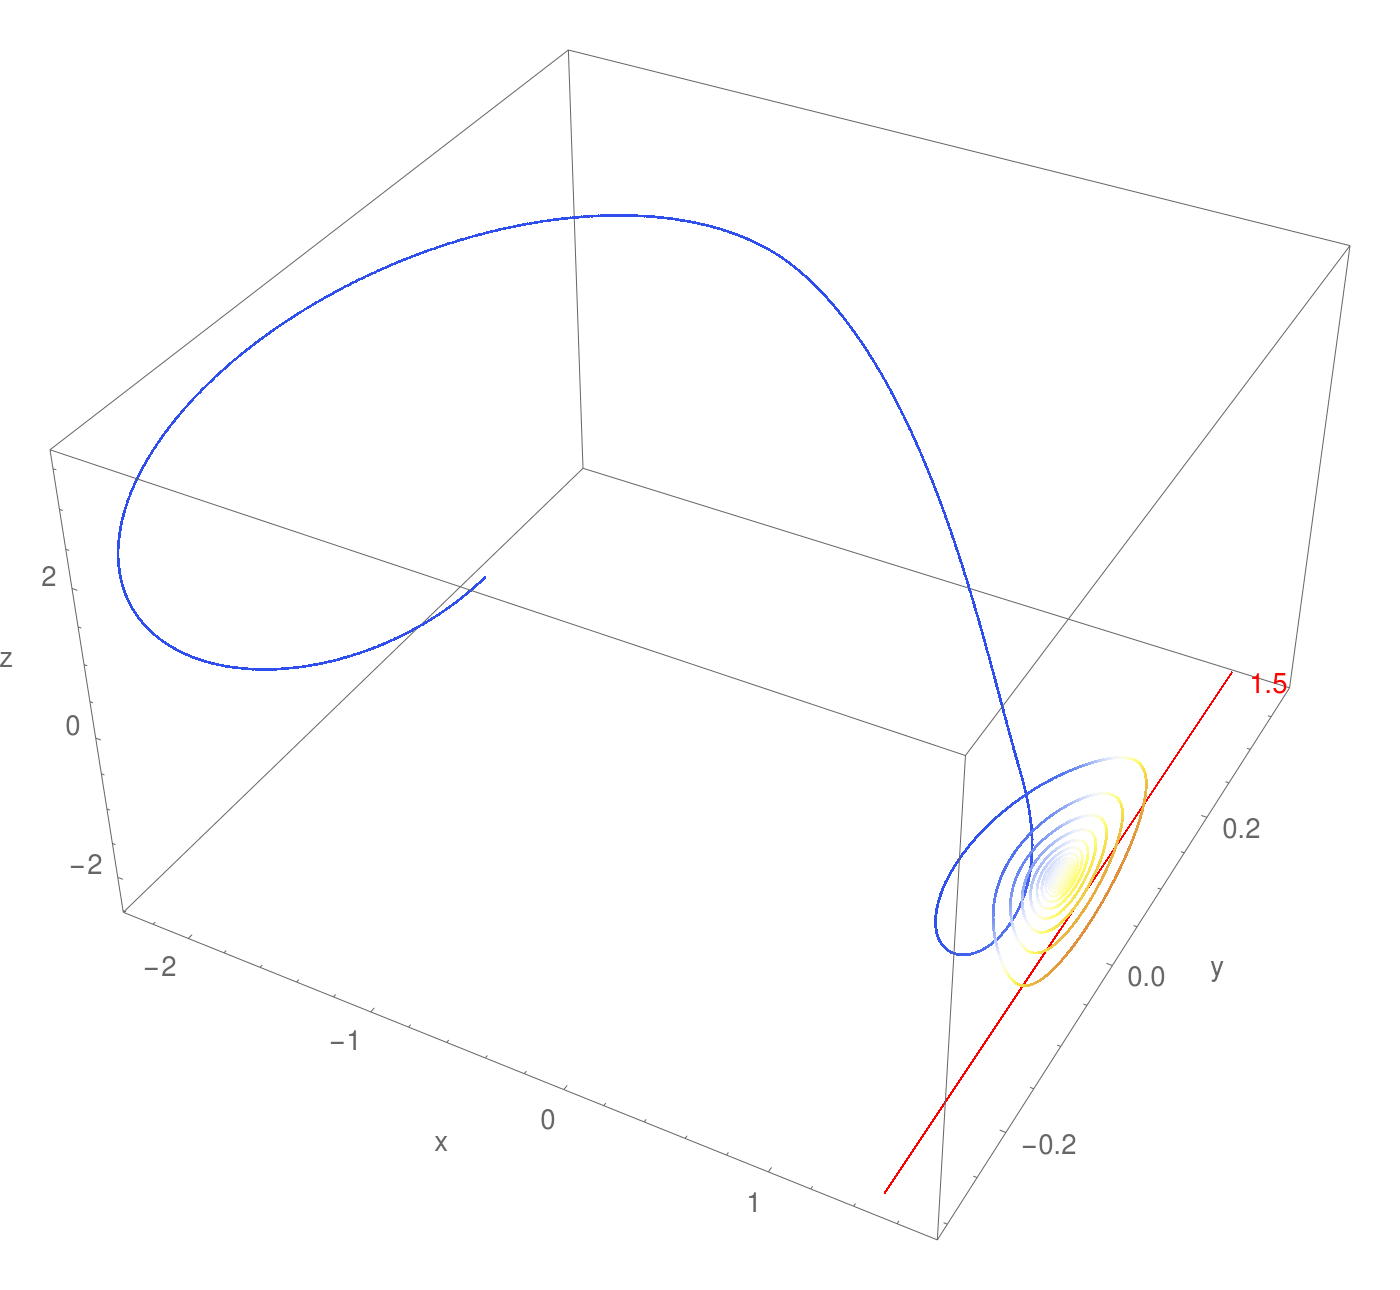
\includegraphics[width=0.45\textwidth]{controllers/chua-circuit/Limited-chua-circuit-x-softness-0-13-1-5-convergence.png}
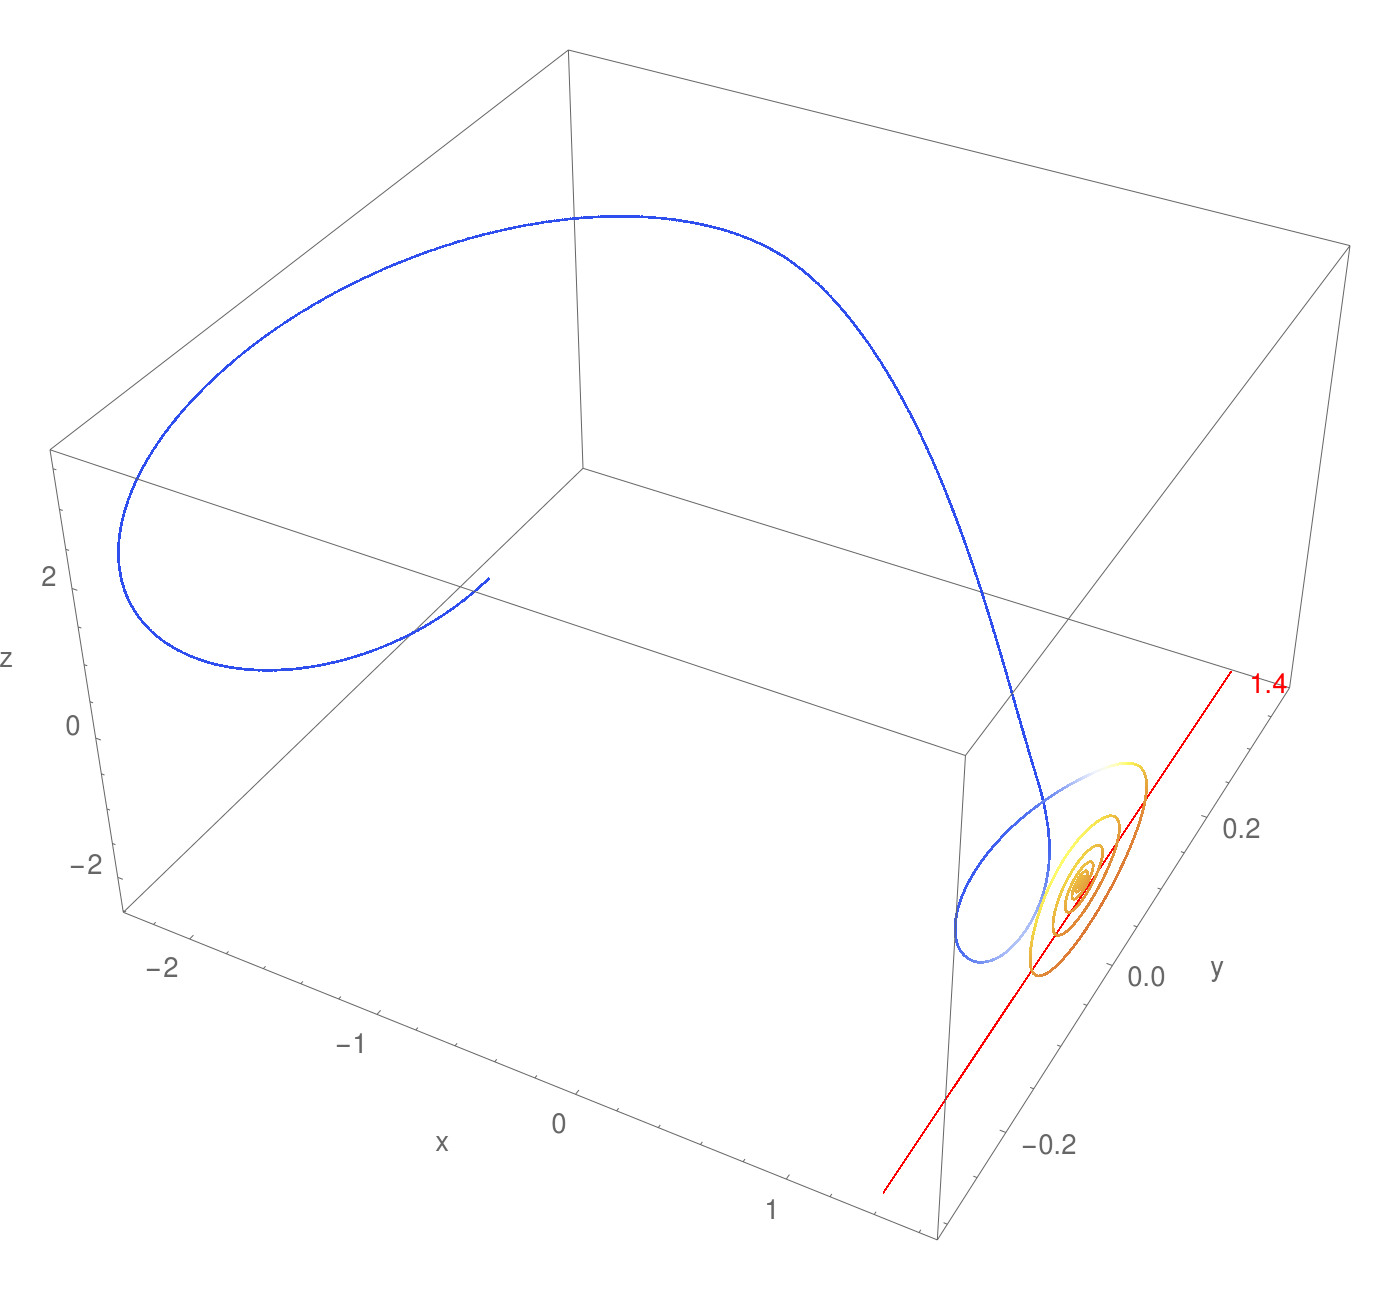
\includegraphics[width=0.45\textwidth]{controllers/chua-circuit/Limited-chua-circuit-x-softness-0-13-1-4-convergence.png}
\caption[Figure of fix point convergence]{Figure of trajectories with limit values 1.5 and 1.4.}
\label{figure:x-0.13-convergence-trajectories}
\end{figure}

Moving the limiter to 1.3 leads to a rotation of the plane in which the original trajectories took place, and an inward spiral starting at the initial conditions and progressing towards the limiter occurs. %
%
The state spiralling into the limiter tries to pass the limiter from the uppermost the gateway scroll to the lowermost scroll.

\begin{figure}[H]
\centering
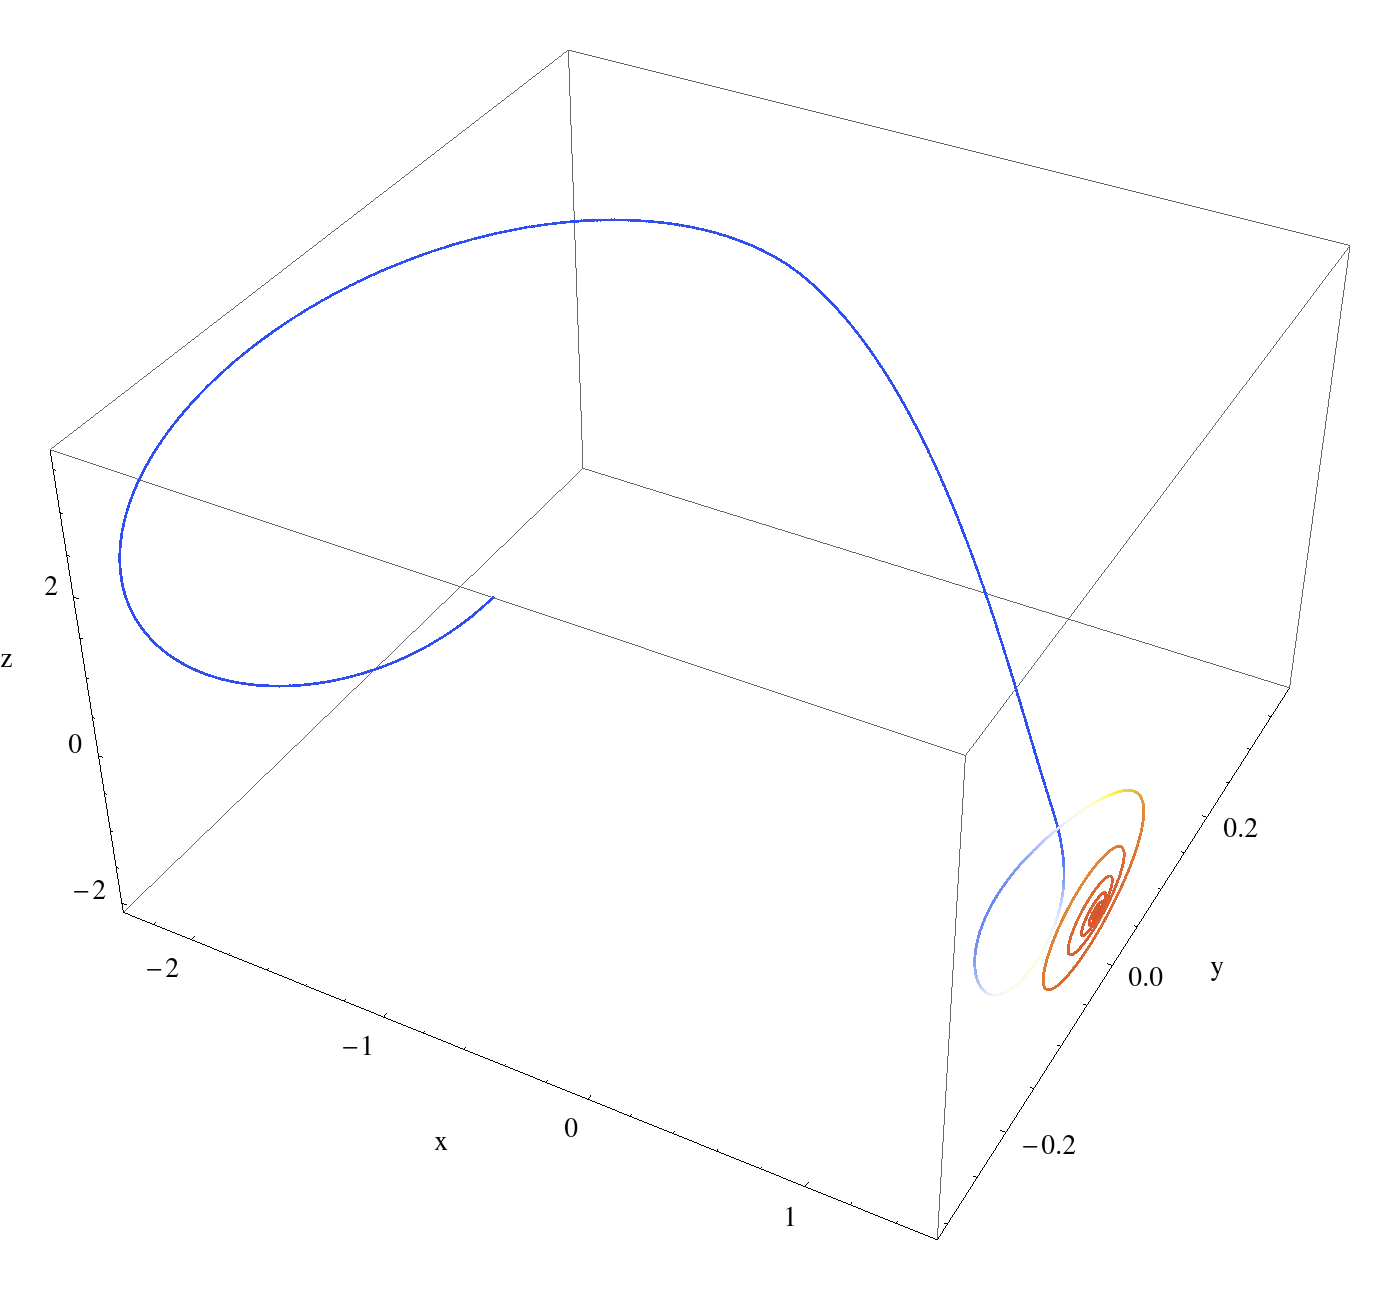
\includegraphics[width=0.45\textwidth]{controllers/chua-circuit/Limited-chua-circuit-x-softness-0-13-1-3-convergence.png}
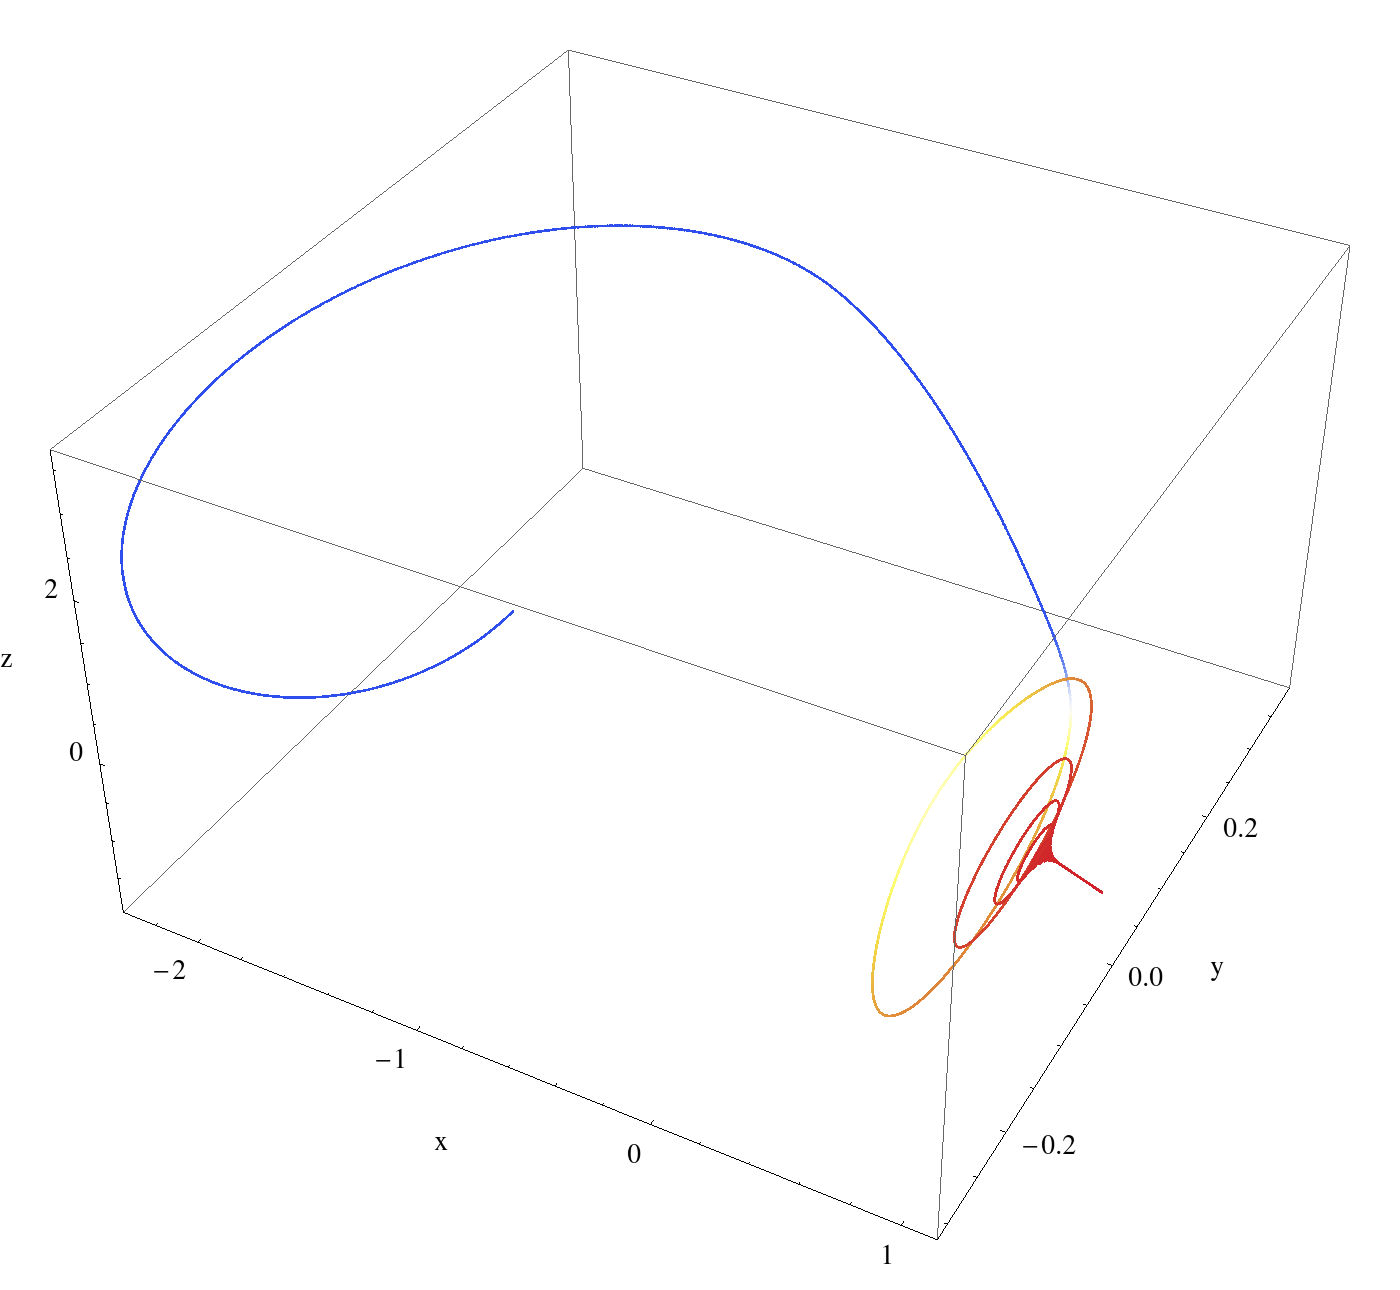
\includegraphics[width=0.45\textwidth]{controllers/chua-circuit/Limited-chua-circuit-x-softness-0-13-0-5-convergence.png}
\caption[Figure of period 1 limit cycle]{Figures of trajectories with limit values 1.3 and 0.5.}
\label{figure:x-0.13-spiral-trajectories}
\end{figure}

The spiralling behavior continues until \(limitValue=0.26991\), where the trajectory stays in the uppermost scroll of the multiscroll attractor before it spirals towards the limiter.

\begin{figure}[H]
\centering
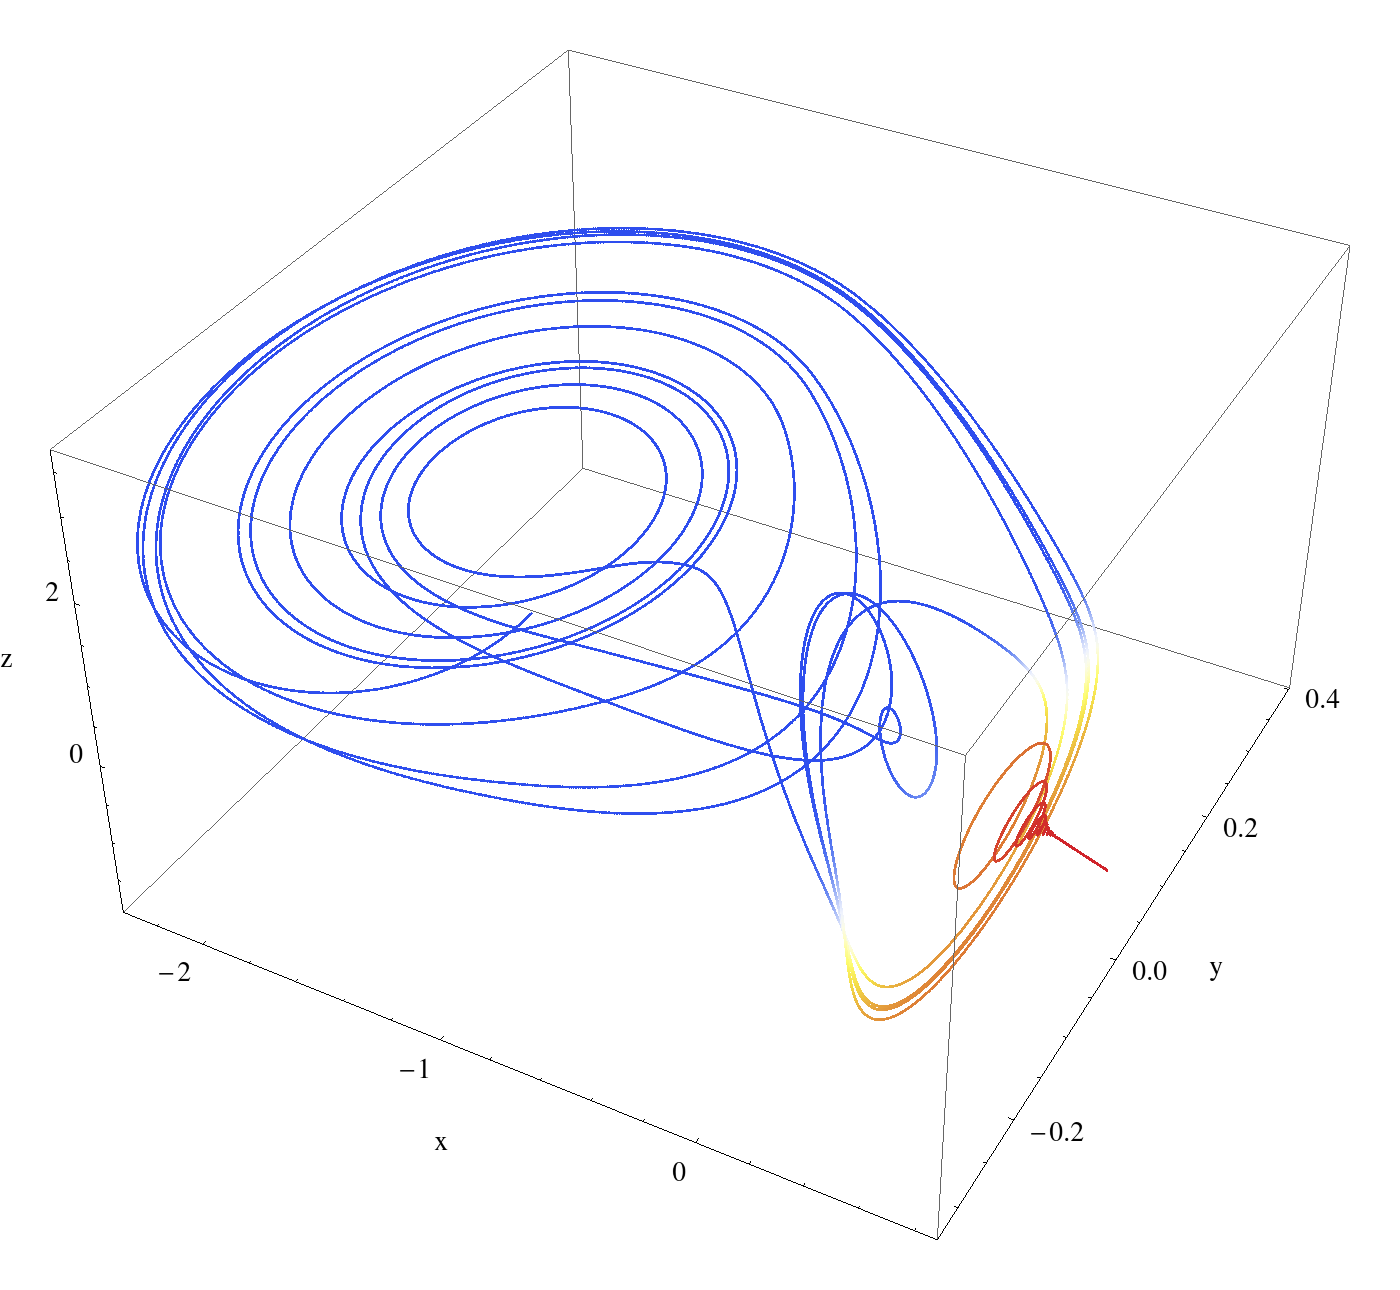
\includegraphics[width=0.8\textwidth]{controllers/chua-circuit/Limited-chua-circuit-x-softness-0-13-0-26991-convergence.png}
\caption[Figure of trajectory with limit value 0.26991.]{Figure the trajectory with limit value 0.26991. The state stays in the uppermost scroll before it spirals into the limiter.}
\label{figure:x-0.13-upper-scroll-trajectory}
\end{figure}

In the uppermost scroll, starting at \(limitValue=0.25304\), one can observe high periodic behavior which can be controlled to different periodicities by moving the limiter towards the scroll. 

\begin{table}[H]
\renewcommand{\arraystretch}{1.2}
\center
\begin{tabular}{@{}ll@{}}
	\toprule
   \(limitValue\) & Limit Cycle\\
   \midrule
   -0.126 & Period 32 \\
   -0.127 & Period 16 \\
   -0.1327 & Period 8 \\ 
   -0.15 & Period 4 \\
   -0.2  & Period 2 \\
   -0.34 & Period 1 \\
   \bottomrule
\end{tabular}
\caption[Limiter values for periodic trajectories for for an x self-limiting limiter with softness 0.13]{Different limit values resulting in trajectories of different periodicity in the uppermost scroll.}
\label{table:x-0.13-periodicities}
\end{table}

\begin{figure}[H]
\centering
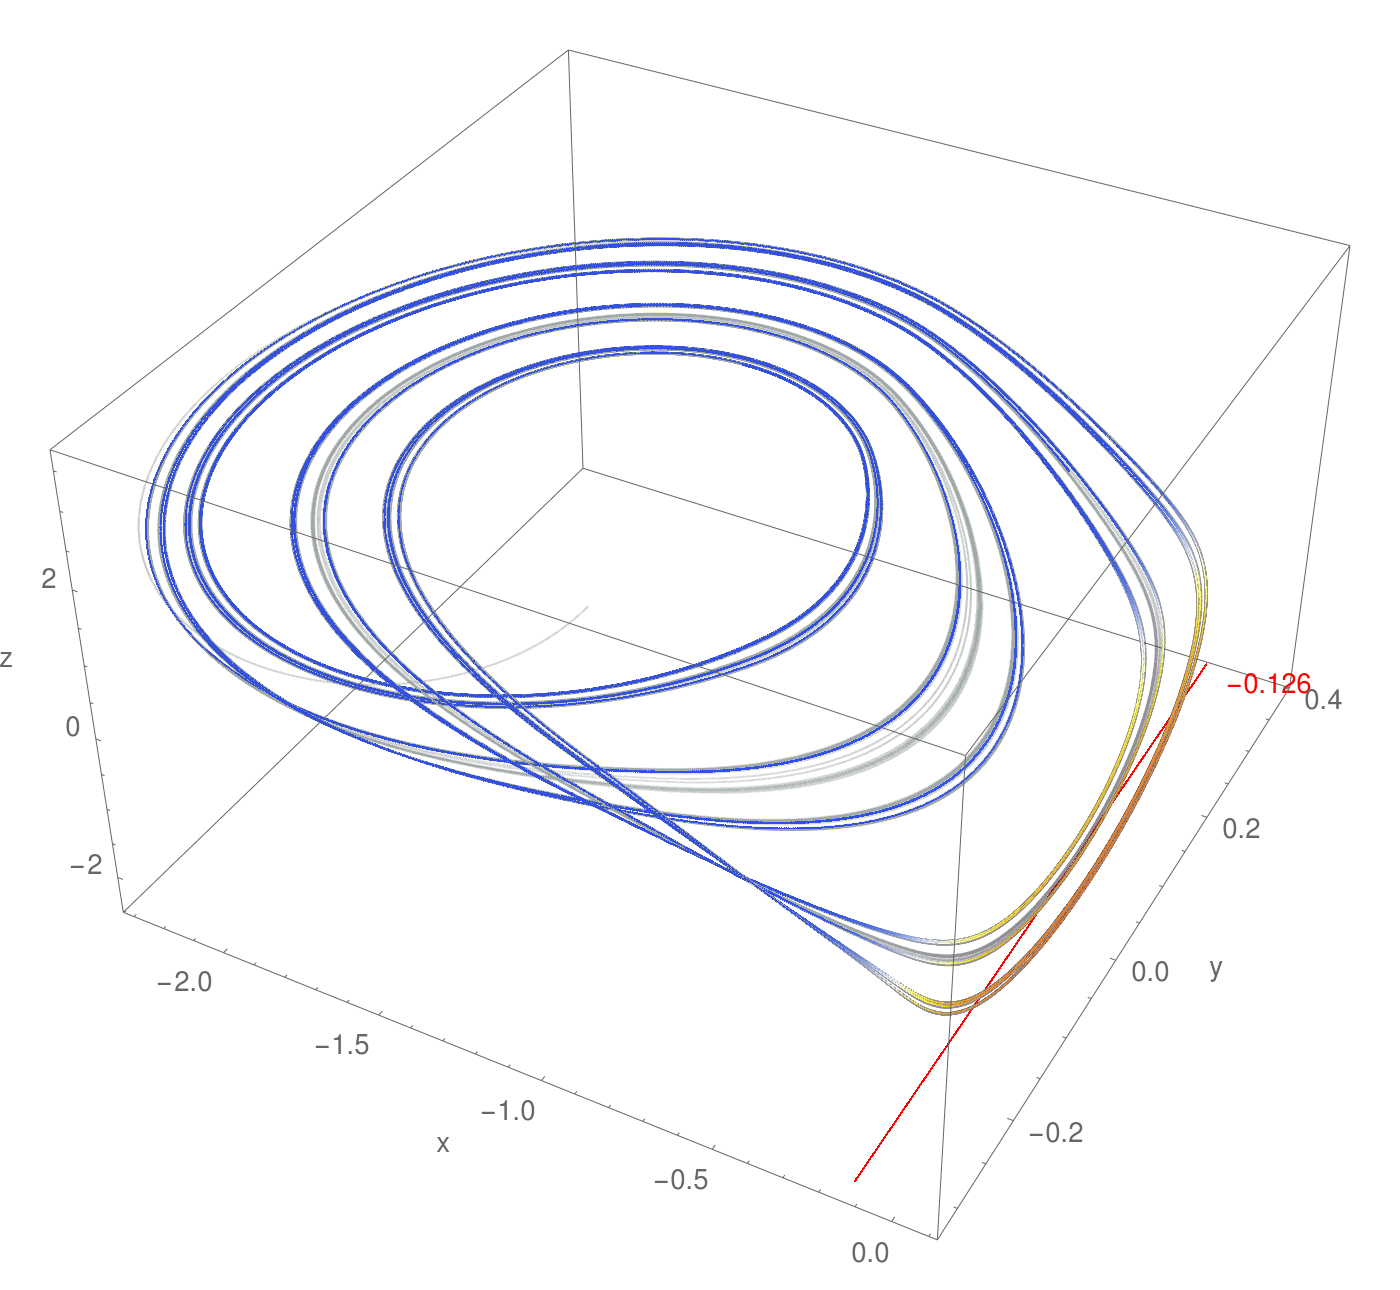
\includegraphics[height=0.45\textheight]{controllers/chua-circuit/Limited-chua-circuit-x-softness-0-13--0-126-convergence.png}
\caption[Figure of period 32 limit cycle]{Figure of period 32 limit cycle in the uppermost scroll using a self limiter with value 0.13.}
\label{figure:x-0.13-32-limit-cycle-upperscroll-trajectory}
\end{figure}

\begin{figure}[H]
\centering
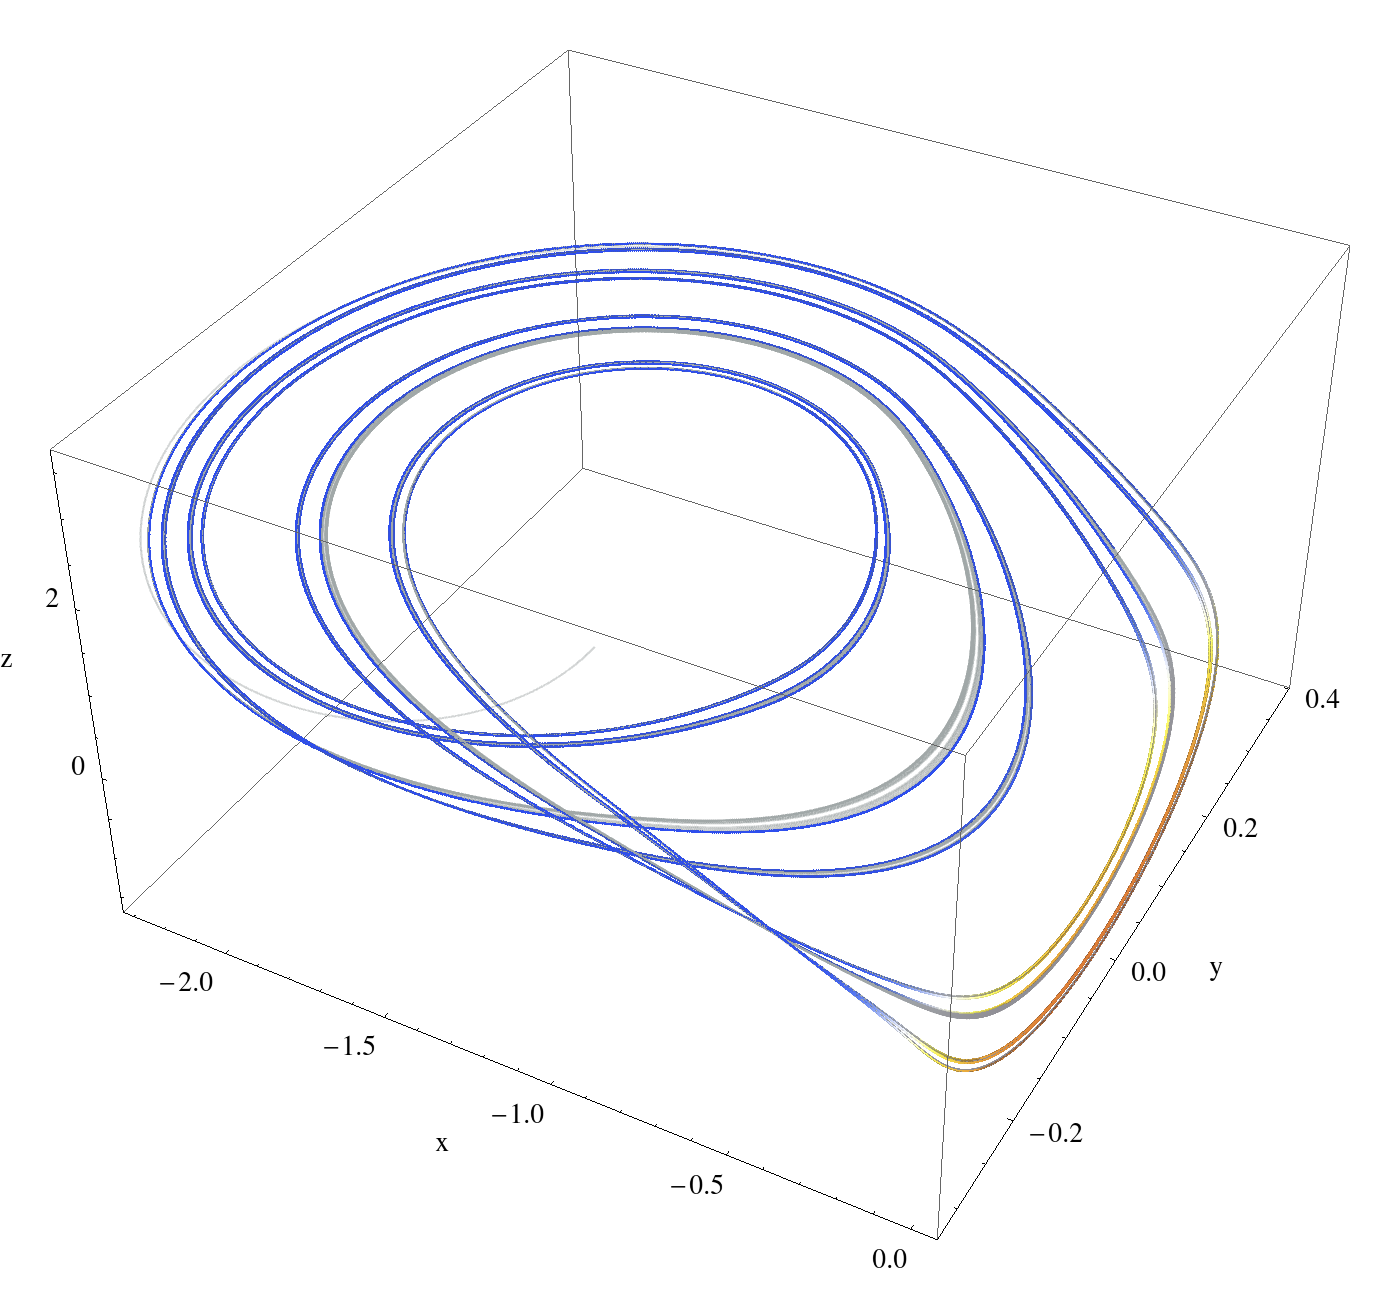
\includegraphics[height=0.45\textheight]{controllers/chua-circuit/Limited-chua-circuit-x-softness-0-13--0-127-convergence.png}
\caption[Figure of period 16 limit cycle]{Figure of period 16 limit cycle in the uppermost scroll using a self limiter with value 0.13.}
\label{figure:x-0.13-16-limit-cycle-upperscroll-trajectory}
\end{figure}

\begin{figure}[H]
\centering
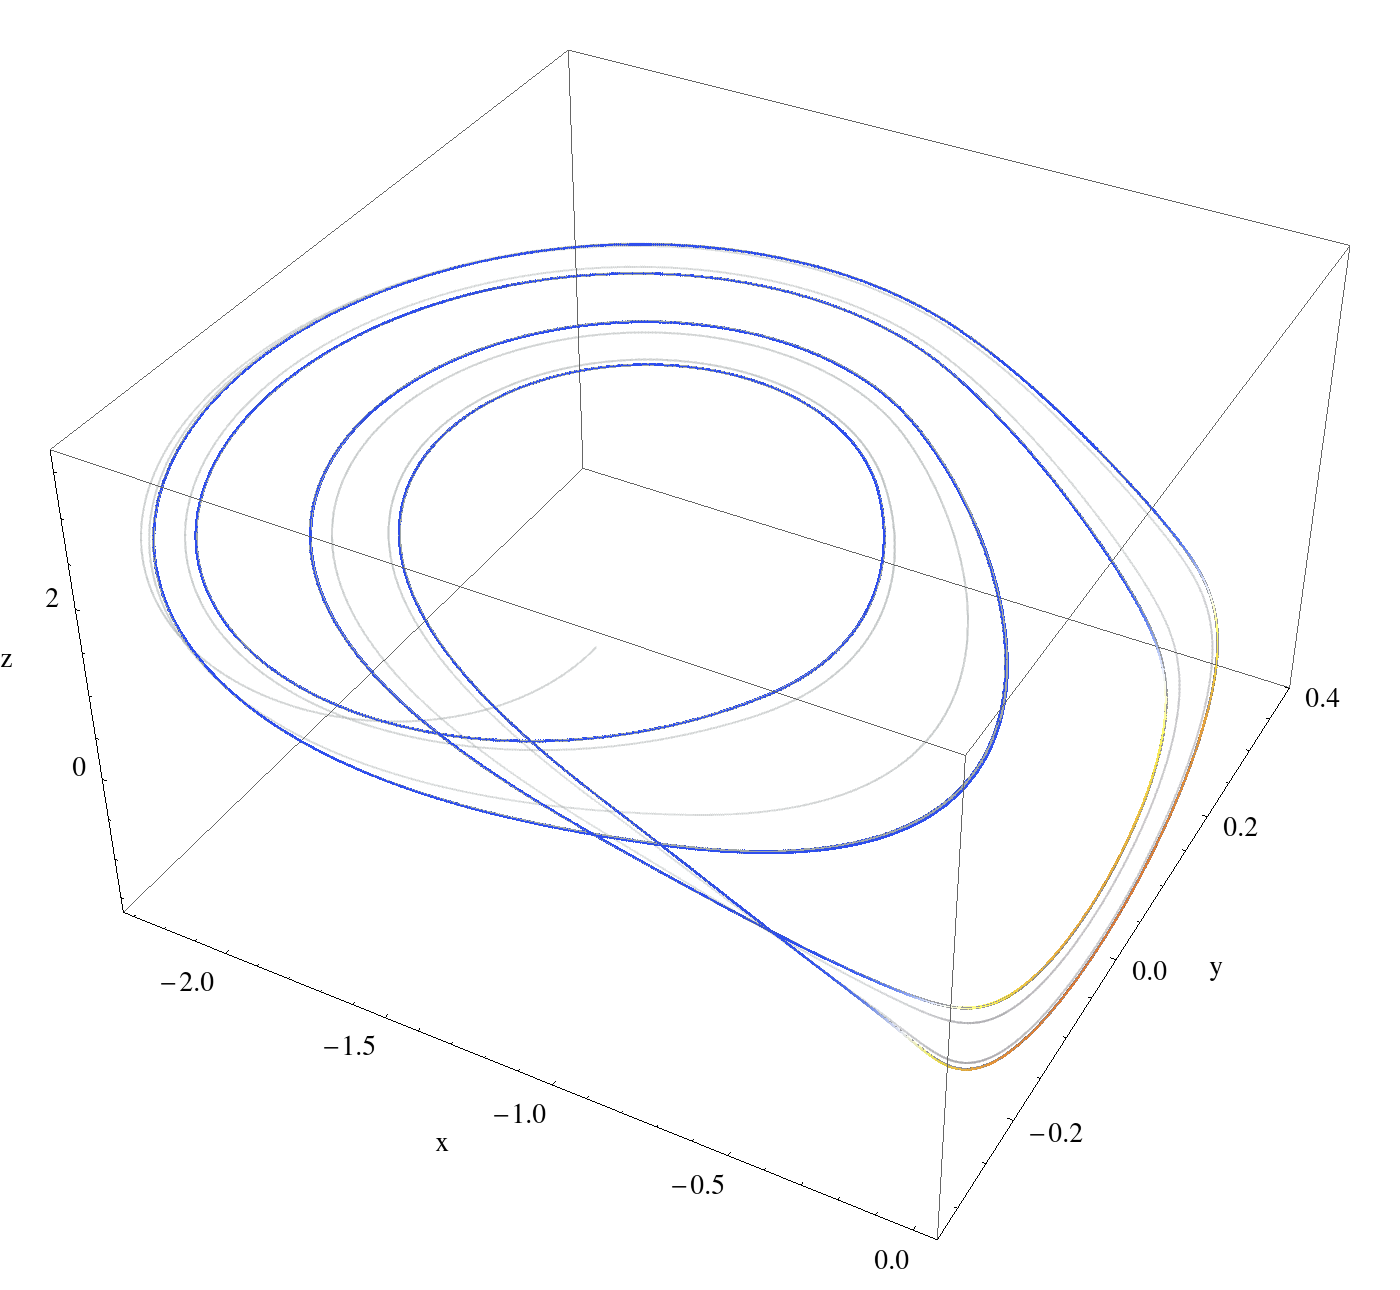
\includegraphics[height=0.45\textheight]{controllers/chua-circuit/Limited-chua-circuit-x-softness-0-13--0-1327-convergence.png}
\caption[Figure of period 8 limit cycle]{Figure of period 8 limit cycle in the uppermost scroll using a self limiter with value 0.13.}
\label{figure:x-0.13-8-limit-cycle-upperscroll-trajectory}
\end{figure}

\begin{figure}[H]
\centering
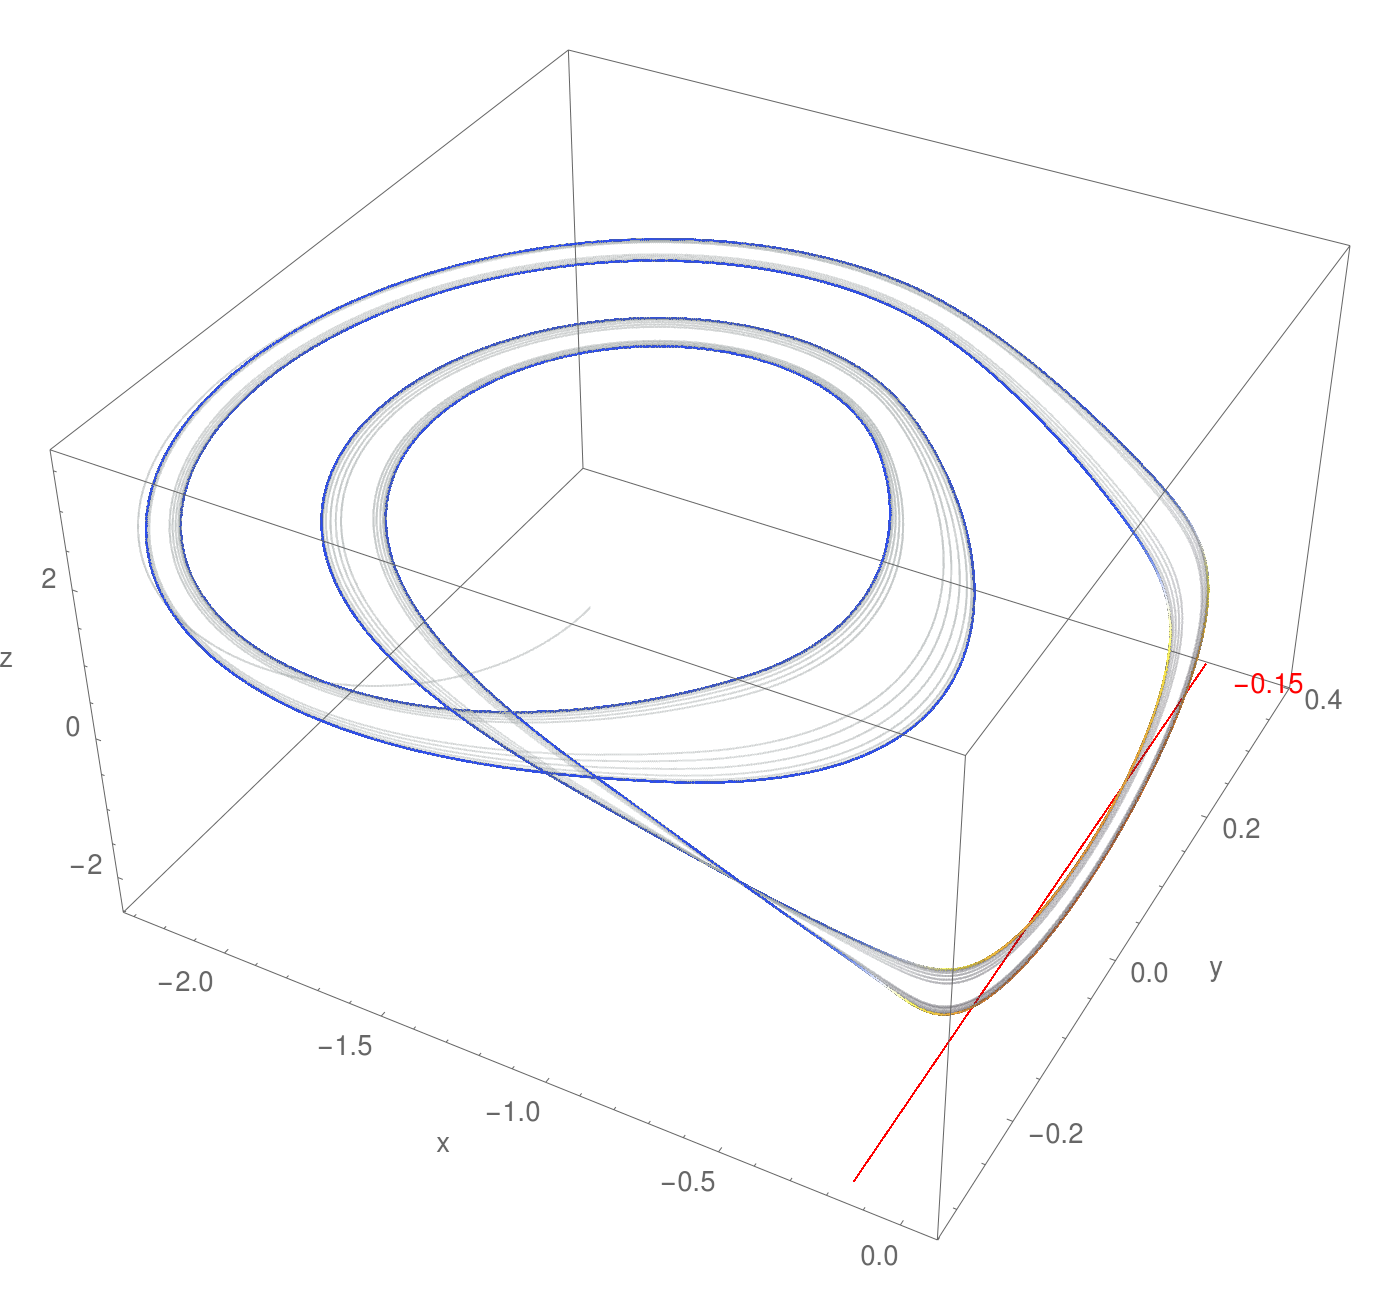
\includegraphics[height=0.45\textheight]{controllers/chua-circuit/Limited-chua-circuit-x-softness-0-13--0-15-convergence.png}
\caption[Figure of period 4 limit cycle]{Figure of period 4 limit cycle in the uppermost scroll using a self limiter with value 0.13.}
\label{figure:x-0.13-4-limit-cycle-upperscroll-trajectory}
\end{figure}

\begin{figure}[H]
\centering
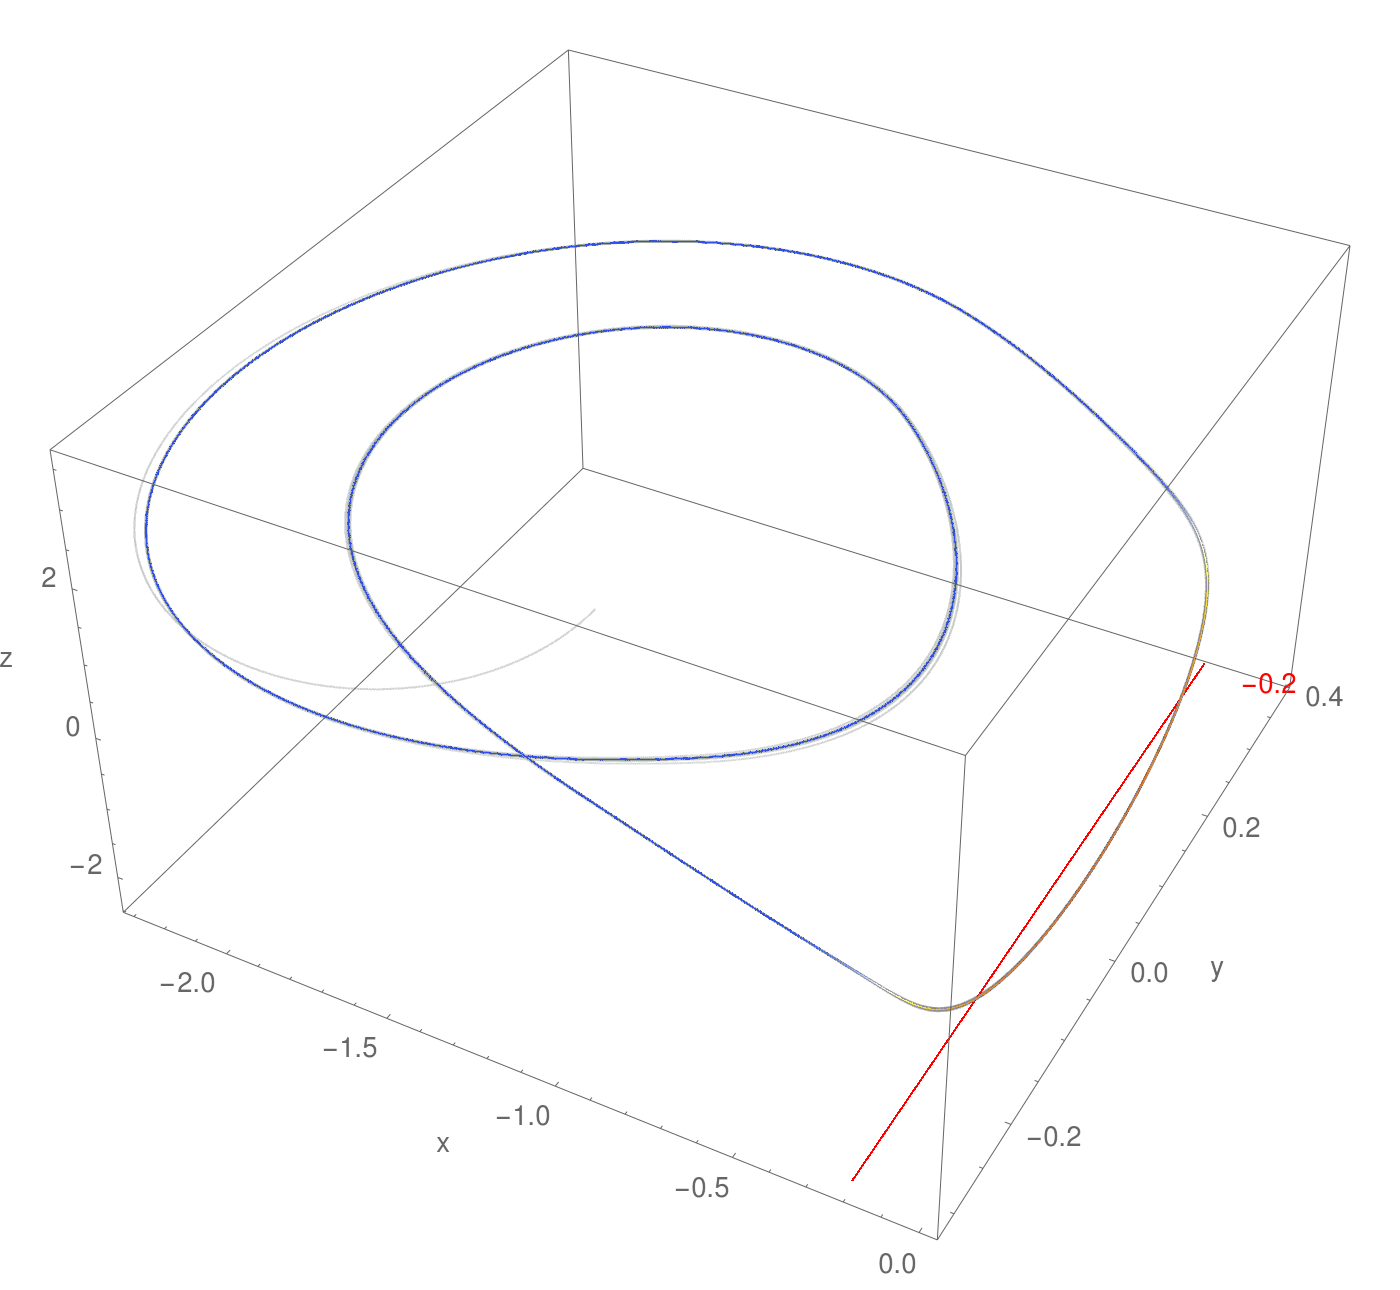
\includegraphics[height=0.45\textheight]{controllers/chua-circuit/Limited-chua-circuit-x-softness-0-13--0-2-convergence.png}
\caption[Figure of period 3 limit cycle]{Figure of period 2 limit cycle in the uppermost scroll using a self limiter with value 0.13.}
\label{figure:x-0.13-2-limit-cycle-upperscroll-trajectory}
\end{figure}

\begin{figure}[H]
\centering
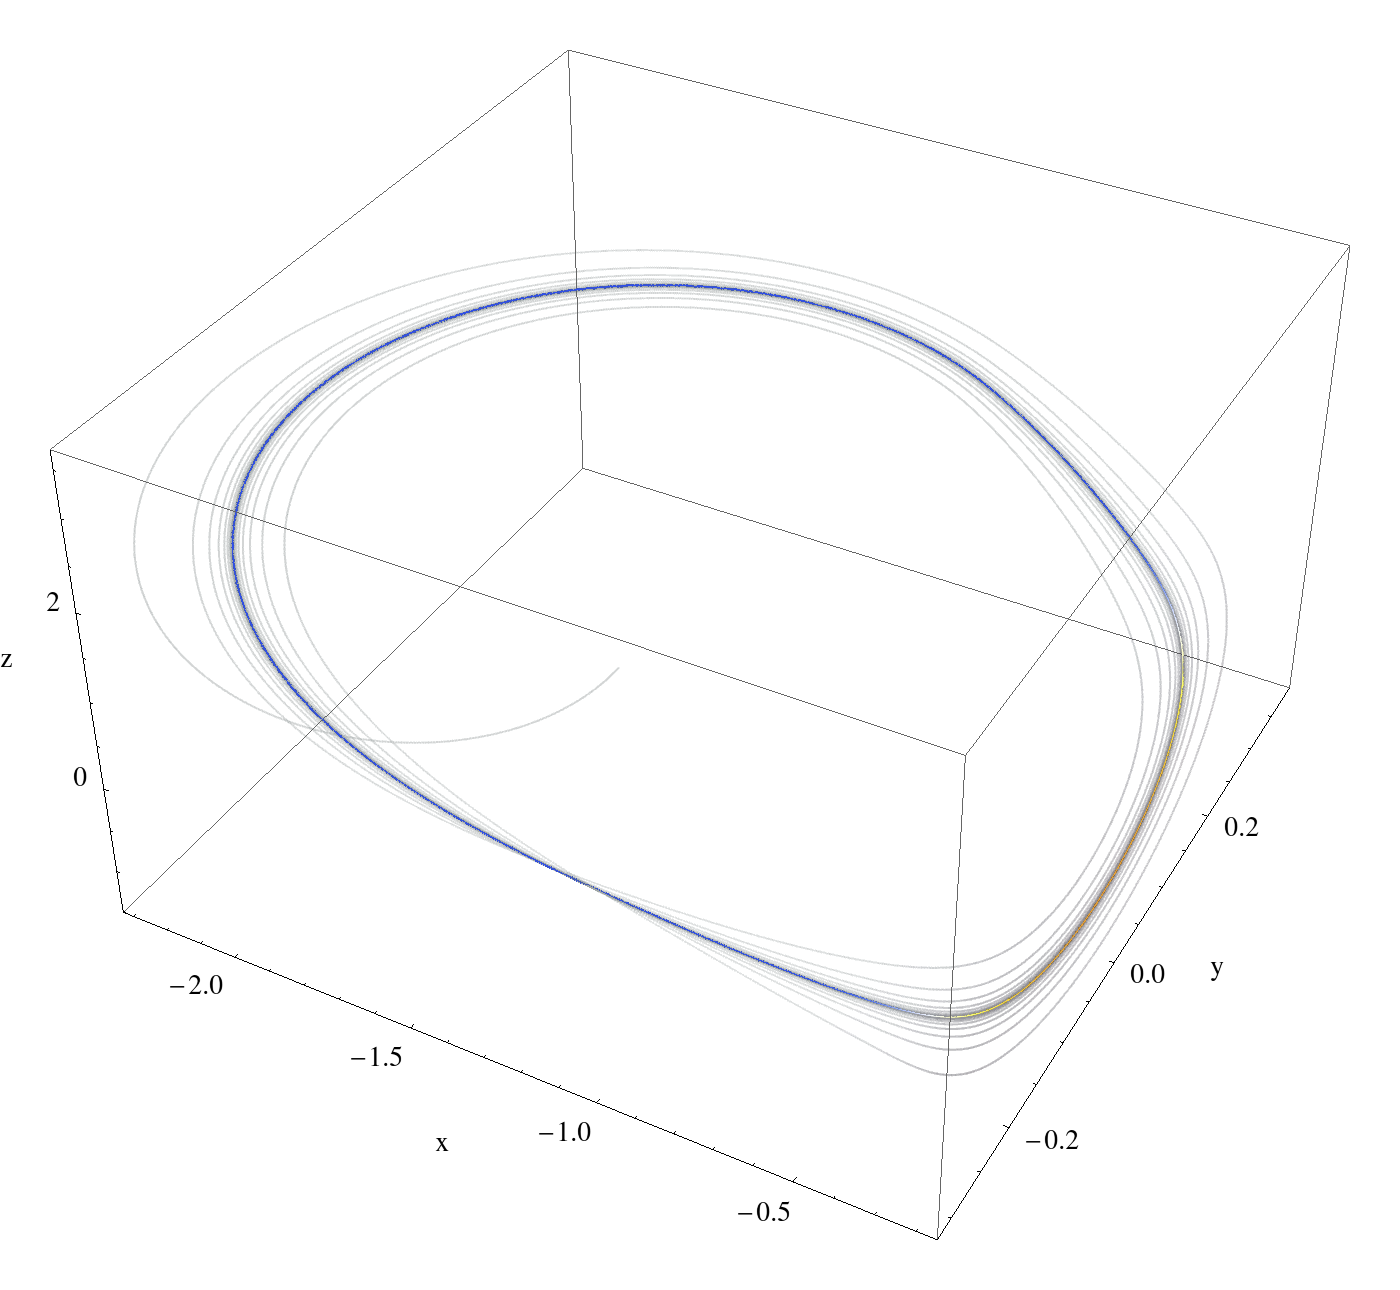
\includegraphics[height=0.45\textheight]{controllers/chua-circuit/Limited-chua-circuit-x-softness-0-13--0-34-convergence.png}
\caption[Figure of period 1 limit cycle]{Figure of period 1 limit cycle in the uppermost scroll.}
\label{figure:x-0.13-1-limit-cycle-upperscroll-trajectory}
\end{figure}

Using \(softness=0.5\), the limiter starts to influence the multiscroll attractor at \(11.507\), and the chaotic behavior can again be controlled using the limiter within the limiter value window \([2.176,11.507]\). %
%
Within the window \([1.8,2.176[\), periodic orbits down to period 1 can be stabilized.

\begin{table}[H]
\renewcommand{\arraystretch}{1.2}
\center
\begin{tabular}{@{}ll@{}}
	\toprule
   \(limitValue\) & Limit Cycle\\
   \midrule
   2.0502 & Period 16 \\
   2.05 & Period 8 \\ 
   2.04 & Period 4 \\
   2  & Period 2 \\
   1.8 & Period 1 \\
   \bottomrule
\end{tabular}
\caption{Different limit values resulting in trajectories of different periodicity}
\label{table:x-0.5-lowermost-periodicities}
\end{table}

\begin{figure}[H]
\centering
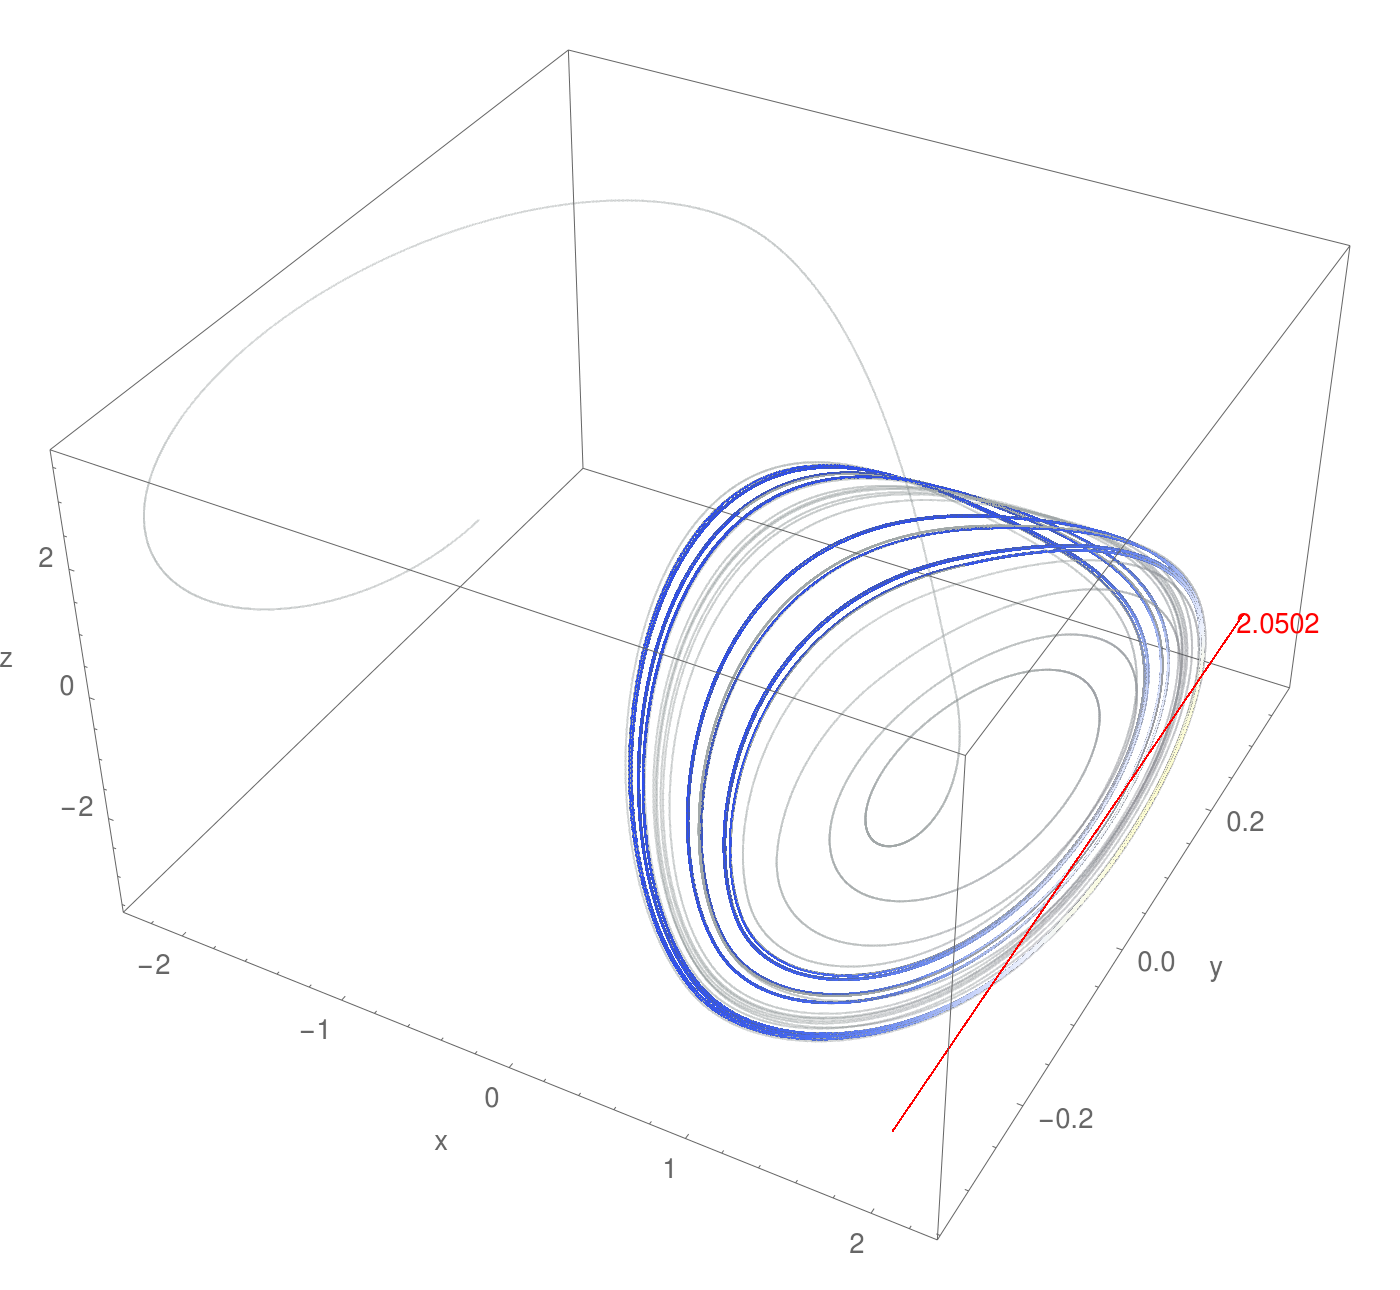
\includegraphics[height=0.45\textheight]{controllers/chua-circuit/Limited-chua-circuit-x-softness-0-5-2-0502-convergence.png}
\caption[Figure of period 16 limit cycle]{Figure of period 16 limit cycle using a self limiter with value 0.5.}
\label{figure:x-0.5-16-limit-cycle-trajectory}
\end{figure}

\begin{figure}[H]
\centering
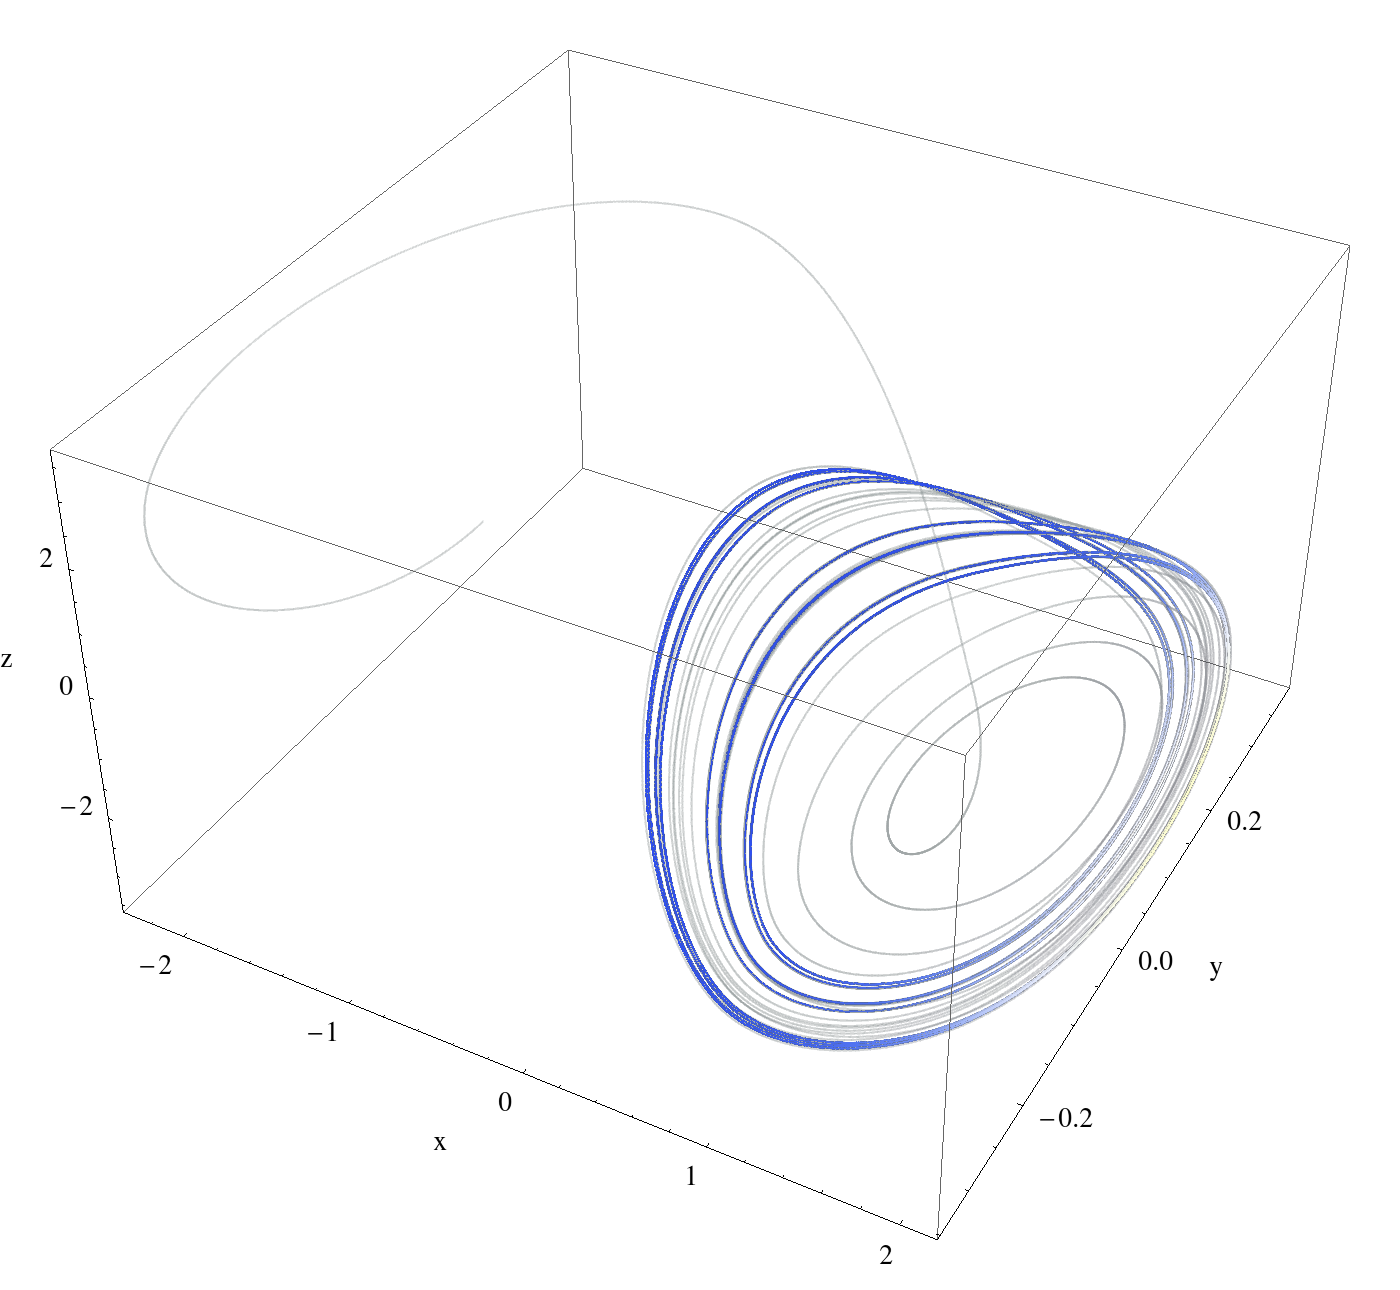
\includegraphics[height=0.45\textheight]{controllers/chua-circuit/Limited-chua-circuit-x-softness-0-5-2-05-convergence.png}
\caption[Figure of period 8 limit cycle]{Figure of period 8 limit cycle using a self limiter with value 0.5.}
\label{figure:x-0.5-8-limit-cycle-trajectory}
\end{figure}

\begin{figure}[H]
\centering
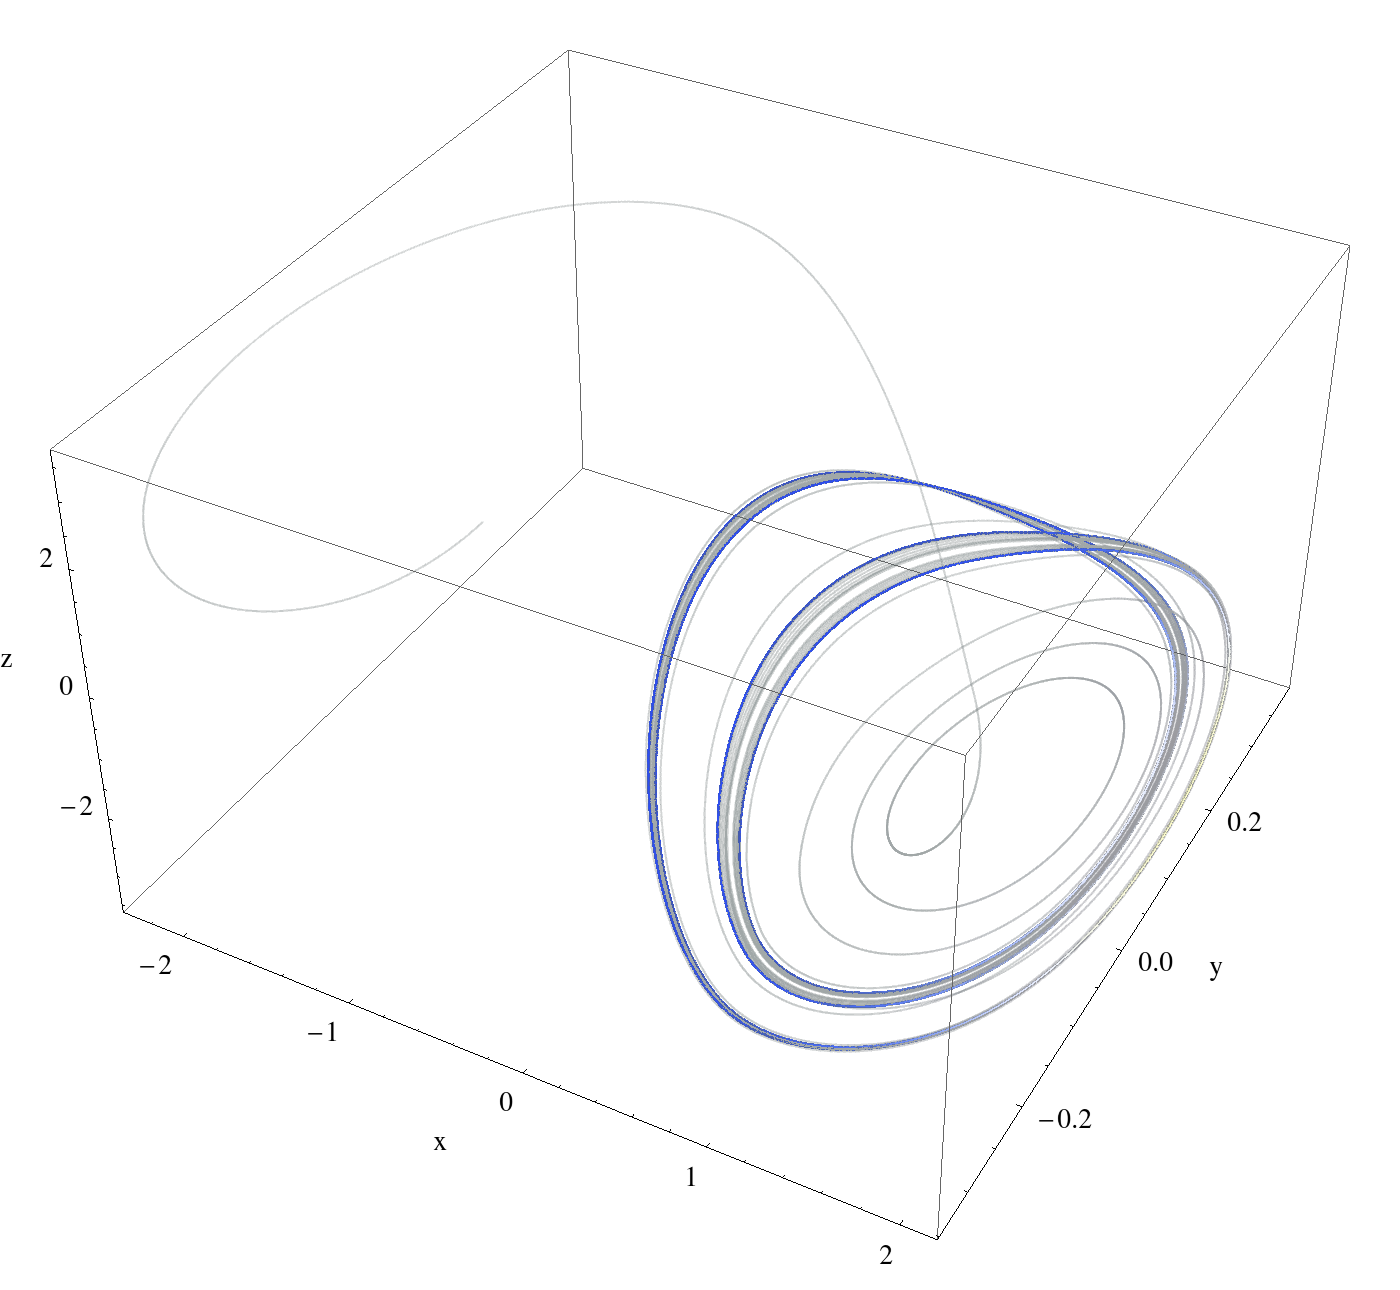
\includegraphics[height=0.45\textheight]{controllers/chua-circuit/Limited-chua-circuit-x-softness-0-5-2-04-convergence.png}
\caption[Figure of period 4 limit cycle]{Figure of period 4 limit cycle using a self limiter with value 0.5.}
\label{figure:x-0.5-4-limit-cycle-trajectory}
\end{figure}

\begin{figure}[H]
\centering
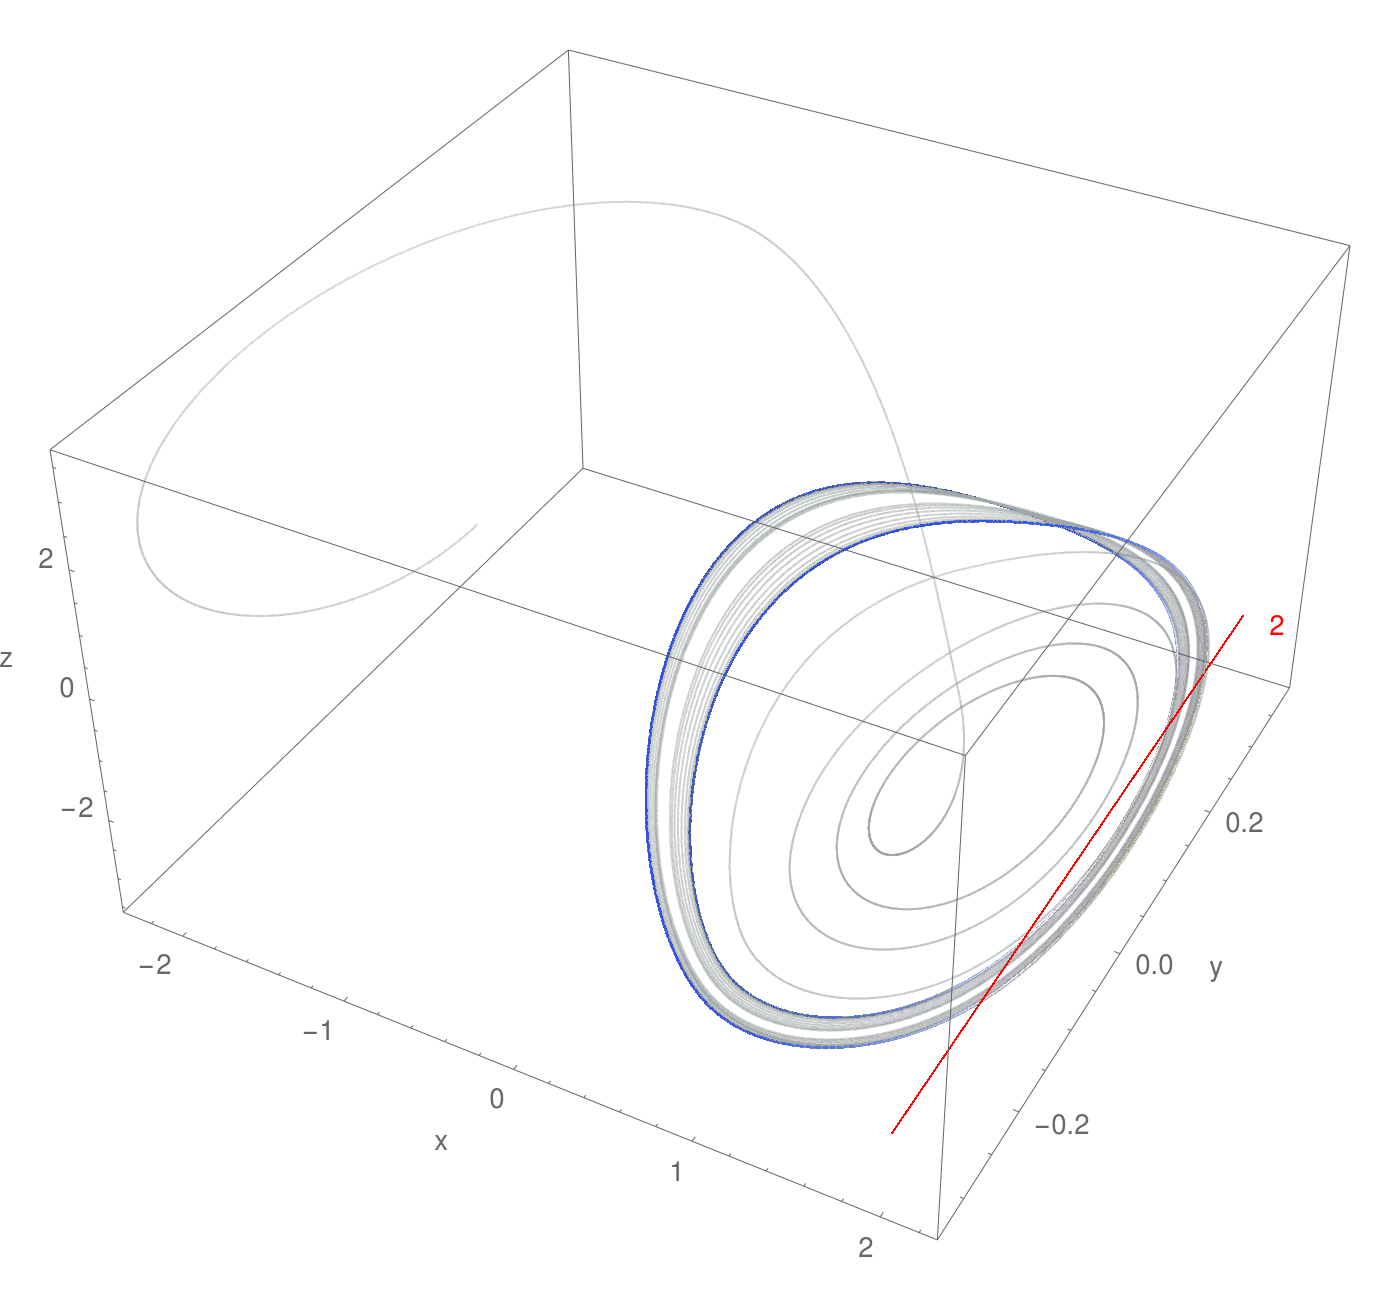
\includegraphics[height=0.45\textheight]{controllers/chua-circuit/Limited-chua-circuit-x-softness-0-5-2-convergence.png}
\caption[Figure of period 2 limit cycle]{Figure of period 2 limit cycle using a self limiter with value 0.5.}
\label{figure:x-0.5-2-limit-cycle-trajectory}
\end{figure}

\begin{figure}[H]
\centering
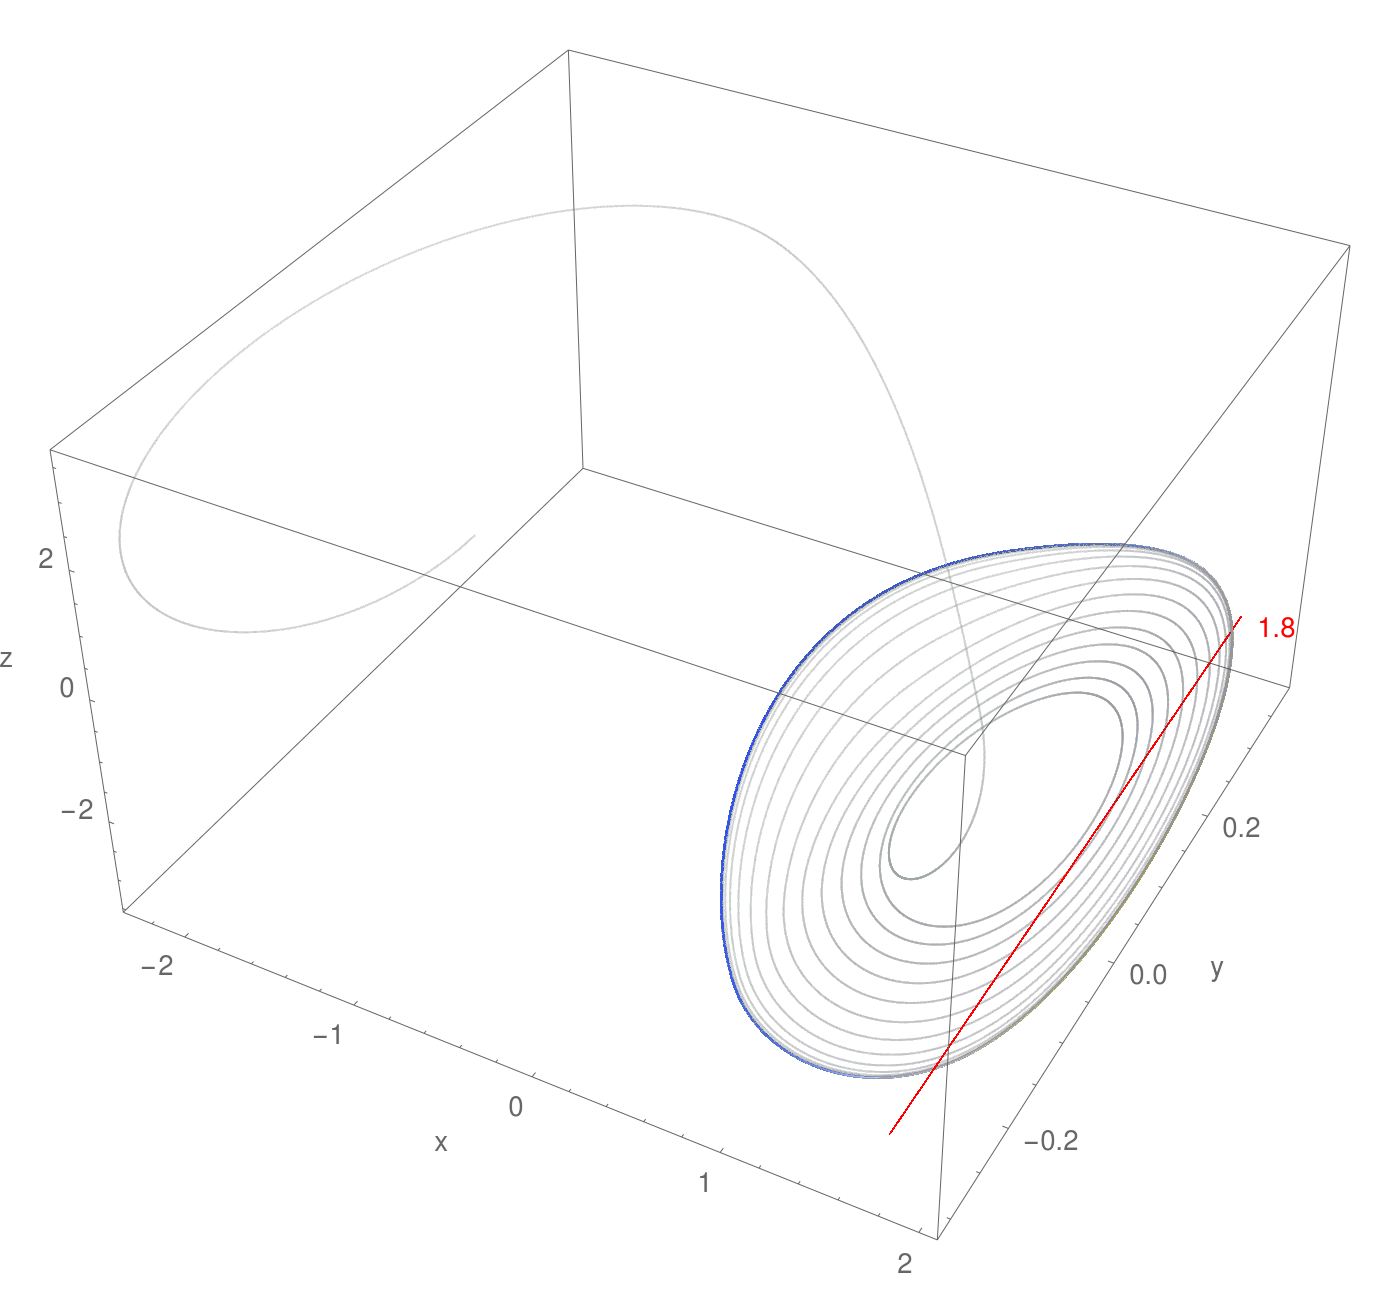
\includegraphics[height=0.45\textheight]{controllers/chua-circuit/Limited-chua-circuit-x-softness-0-5-1-8-convergence.png}
\caption[Figure of period 1 limit cycle]{Figure of period 1 limit cycle using a self limiter with value 0.5.}
\label{figure:x-0.5-1-limit-cycle-trajectory}
\end{figure}

The limit parameter can again be set beyond 0. The same plane rotation and spiralling behaviour can be seen, until it stays in the trajectory stays in the uppermost scroll of the multiscroll attractor before it spirals towards the limiter. %
%
There the trajectory can again be stabilized in the uppermost scroll into different periodic orbits (see table \ref{table:x-0.5-upperscroll-periodicities}).

\begin{table}[H]
\renewcommand{\arraystretch}{1.2}
\center
\begin{tabular}{@{}ll@{}}
	\toprule
   \(limitValue\) & Limit Cycle\\
   \midrule
   -0.109 & Period 16 \\
   -0.115 & Period 8 \\ 
   -0.15 & Period 4 \\
   -0.2  & Period 2 \\
   -0.37 & Period 1 \\
   \bottomrule
\end{tabular}
\caption[Limiter values for periodic trajectories for for an x self-limiting limiter with softness 0.13]{Different limit values resulting in trajectories of different periodicity in the uppermost scroll.}
\label{table:x-0.5-upperscroll-periodicities}
\end{table}

\begin{figure}[H]
\centering
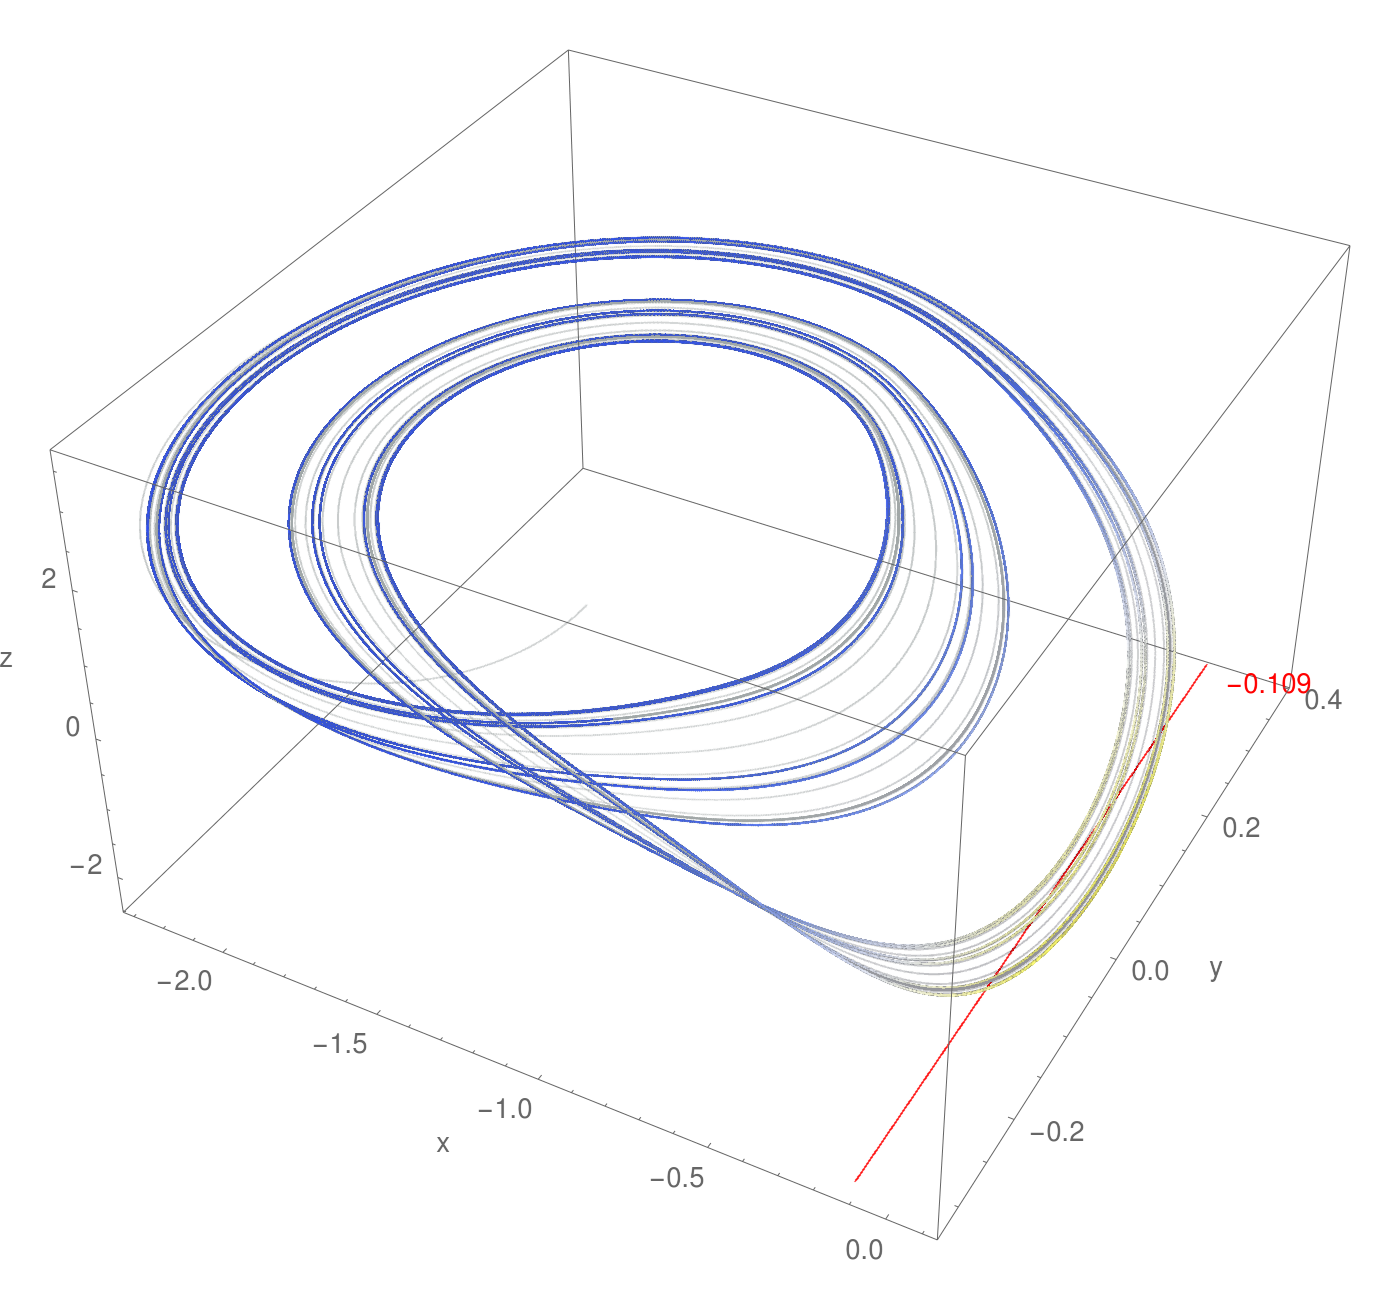
\includegraphics[height=0.45\textheight]{controllers/chua-circuit/Limited-chua-circuit-x-softness-0-5--0-109-convergence.png}
\caption[Figure of period 16 limit cycle]{Figure of period 16 limit cycle in the uppermost scroll using a self limiter with value 0.5.}
\label{figure:x-0.5-16-limit-cycle-upperscroll-trajectory}
\end{figure}

\begin{figure}[H]
\centering
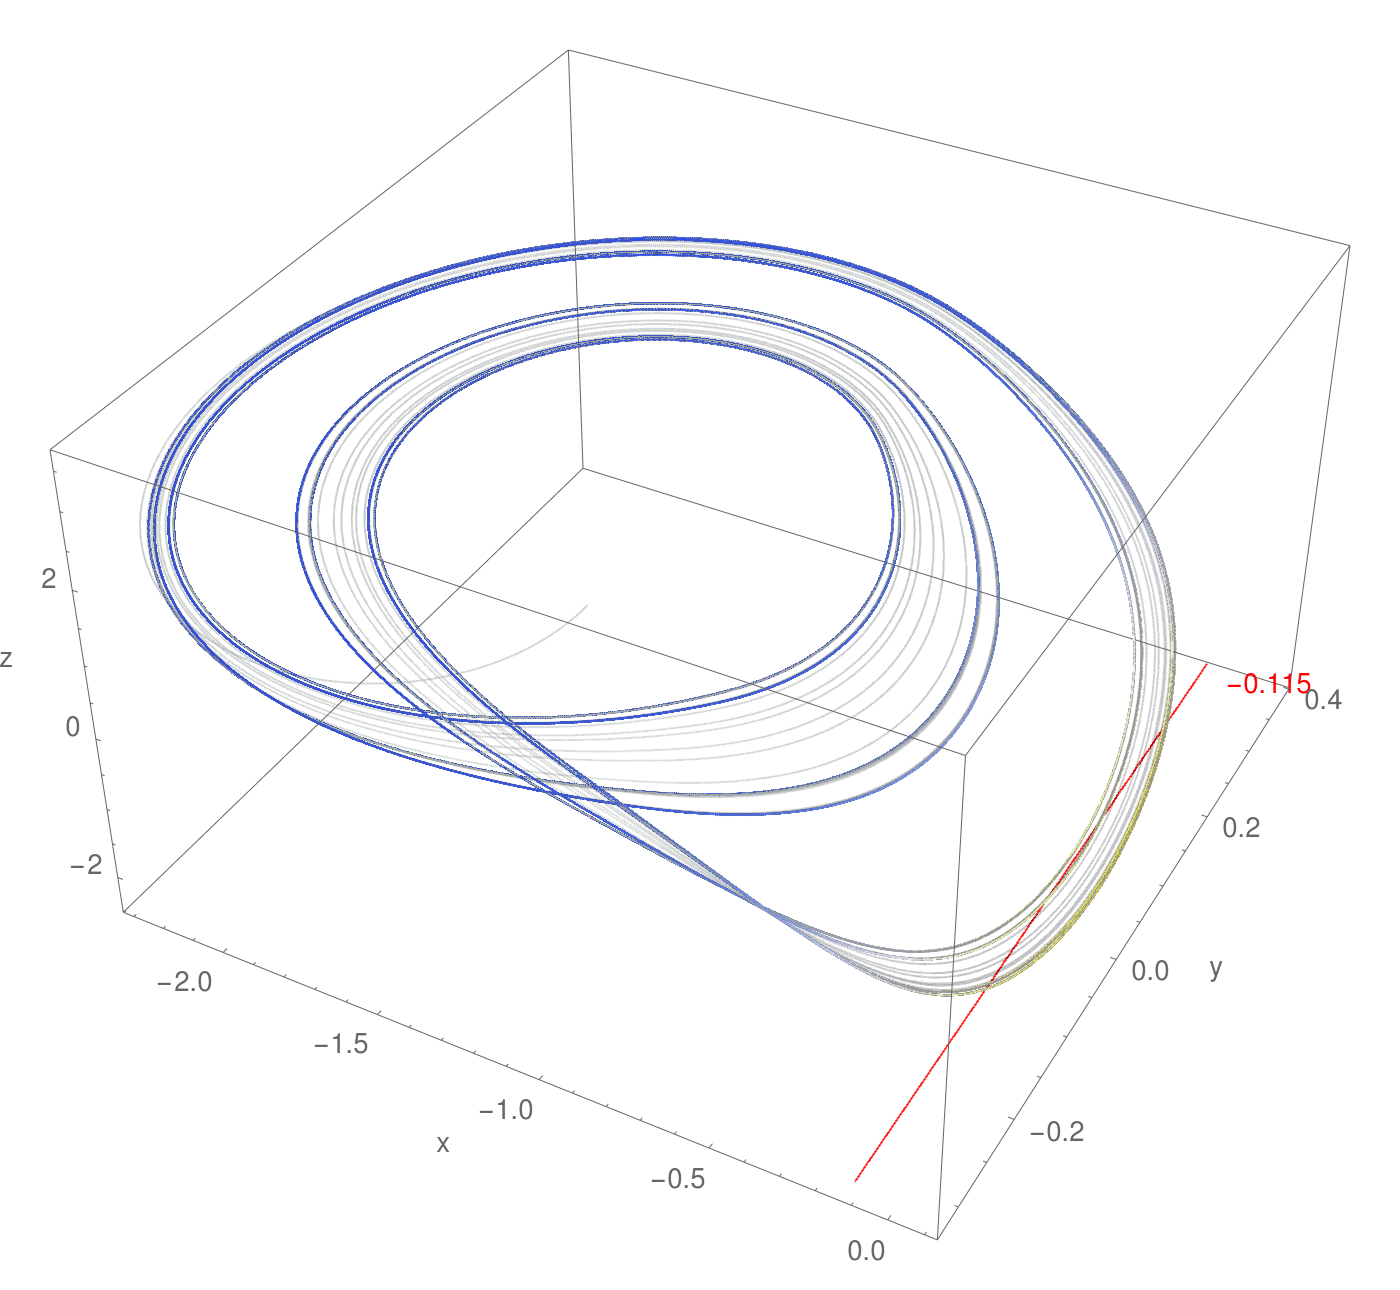
\includegraphics[height=0.45\textheight]{controllers/chua-circuit/Limited-chua-circuit-x-softness-0-5--0-115-convergence.png}
\caption[Figure of period 8 limit cycle]{Figure of period 8 limit cycle in the uppermost scroll using a self limiter with value 0.5.}
\label{figure:x-0.5-8-limit-cycle-upperscroll-trajectory}
\end{figure}

\begin{figure}[H]
\centering
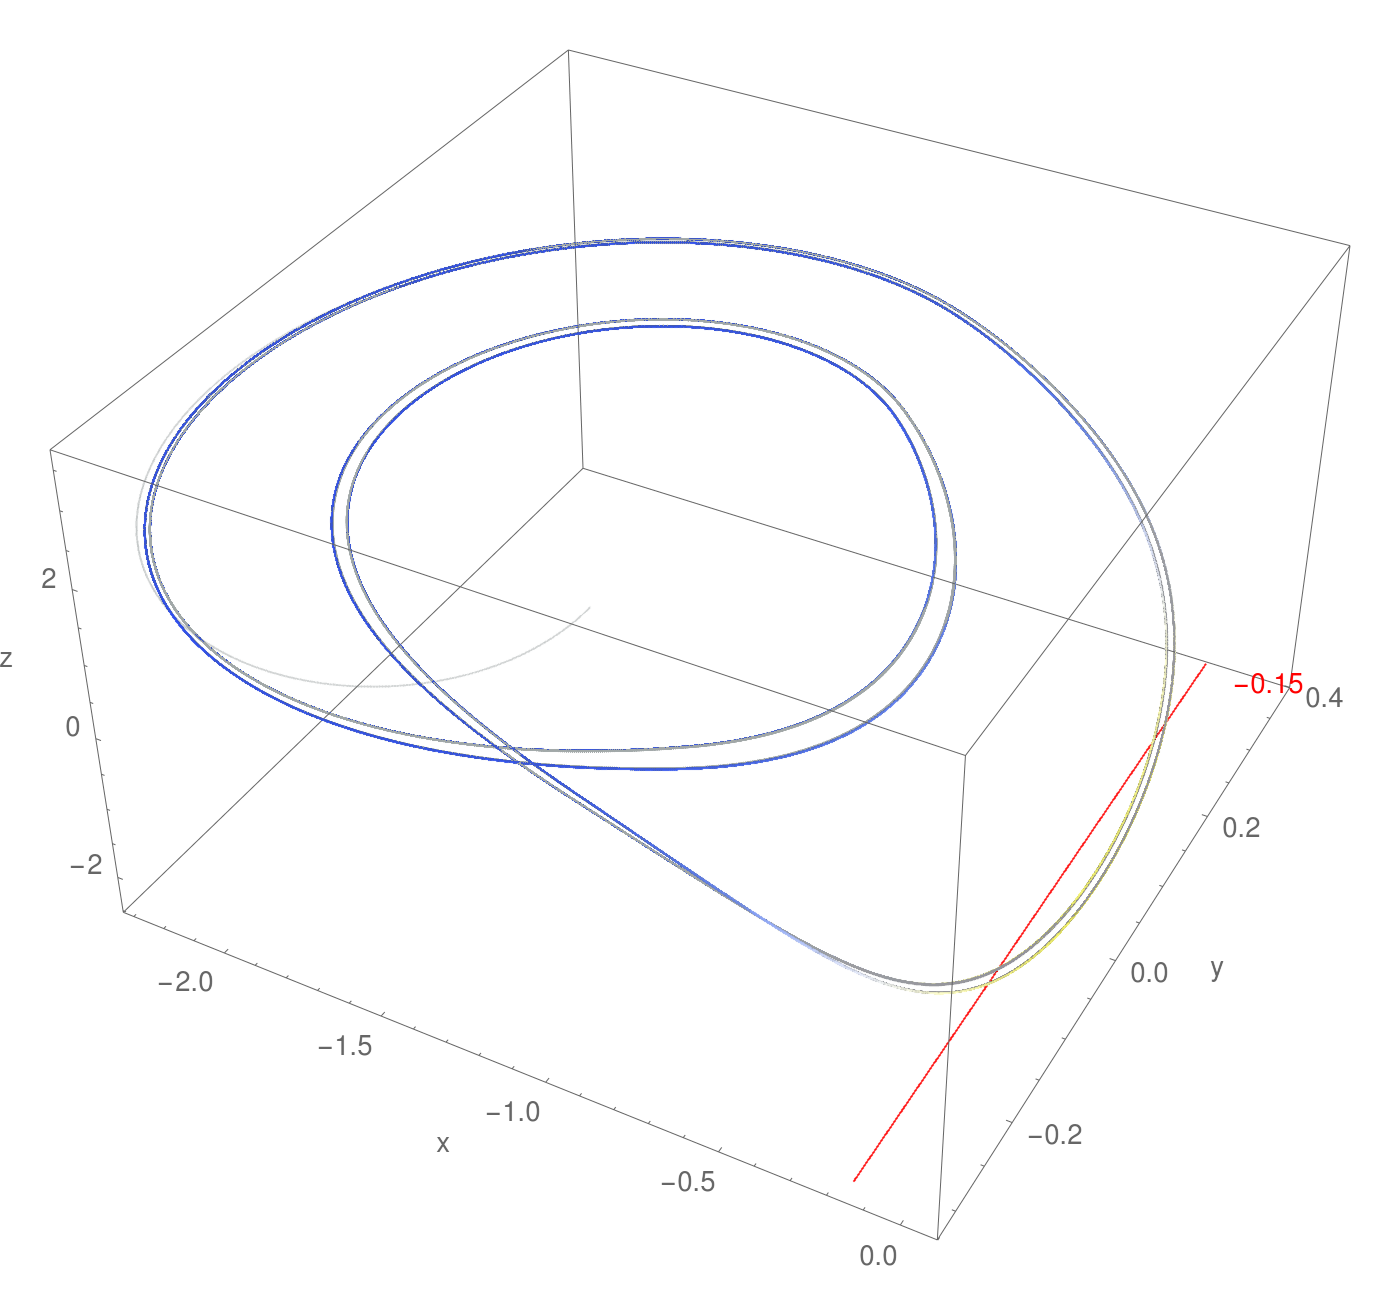
\includegraphics[height=0.45\textheight]{controllers/chua-circuit/Limited-chua-circuit-x-softness-0-5--0-15-convergence.png}
\caption[Figure of period 4 limit cycle]{Figure of period 4 limit cycle in the uppermost scroll using a self limiter with value 0.5.}
\label{figure:x-0.5-4-limit-cycle-upperscroll-trajectory}
\end{figure}

\begin{figure}[H]
\centering
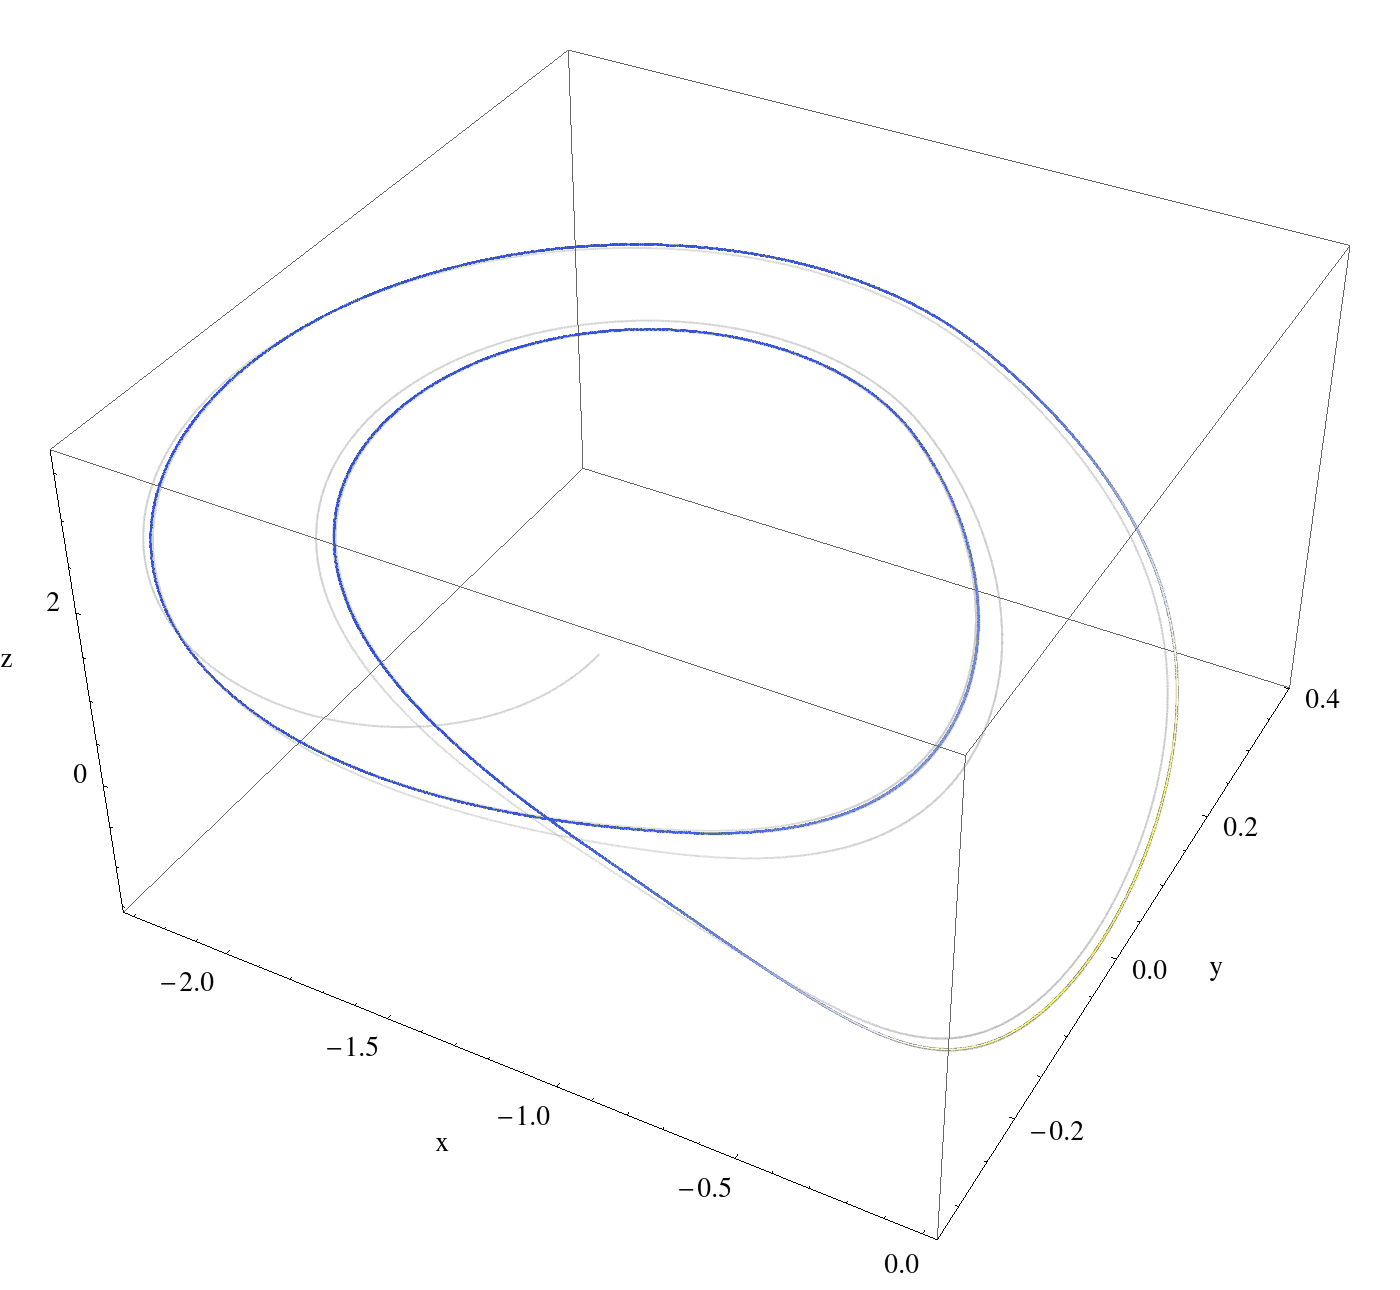
\includegraphics[height=0.45\textheight]{controllers/chua-circuit/Limited-chua-circuit-x-softness-0-5--0-2-convergence.png}
\caption[Figure of period 2 limit cycle]{Figure of period 2 limit cycle in the uppermost scroll using a self limiter with value 0.5.}
\label{figure:x-0.5-2-limit-cycle-upperscroll-trajectory}
\end{figure}

\begin{figure}[H]
\centering
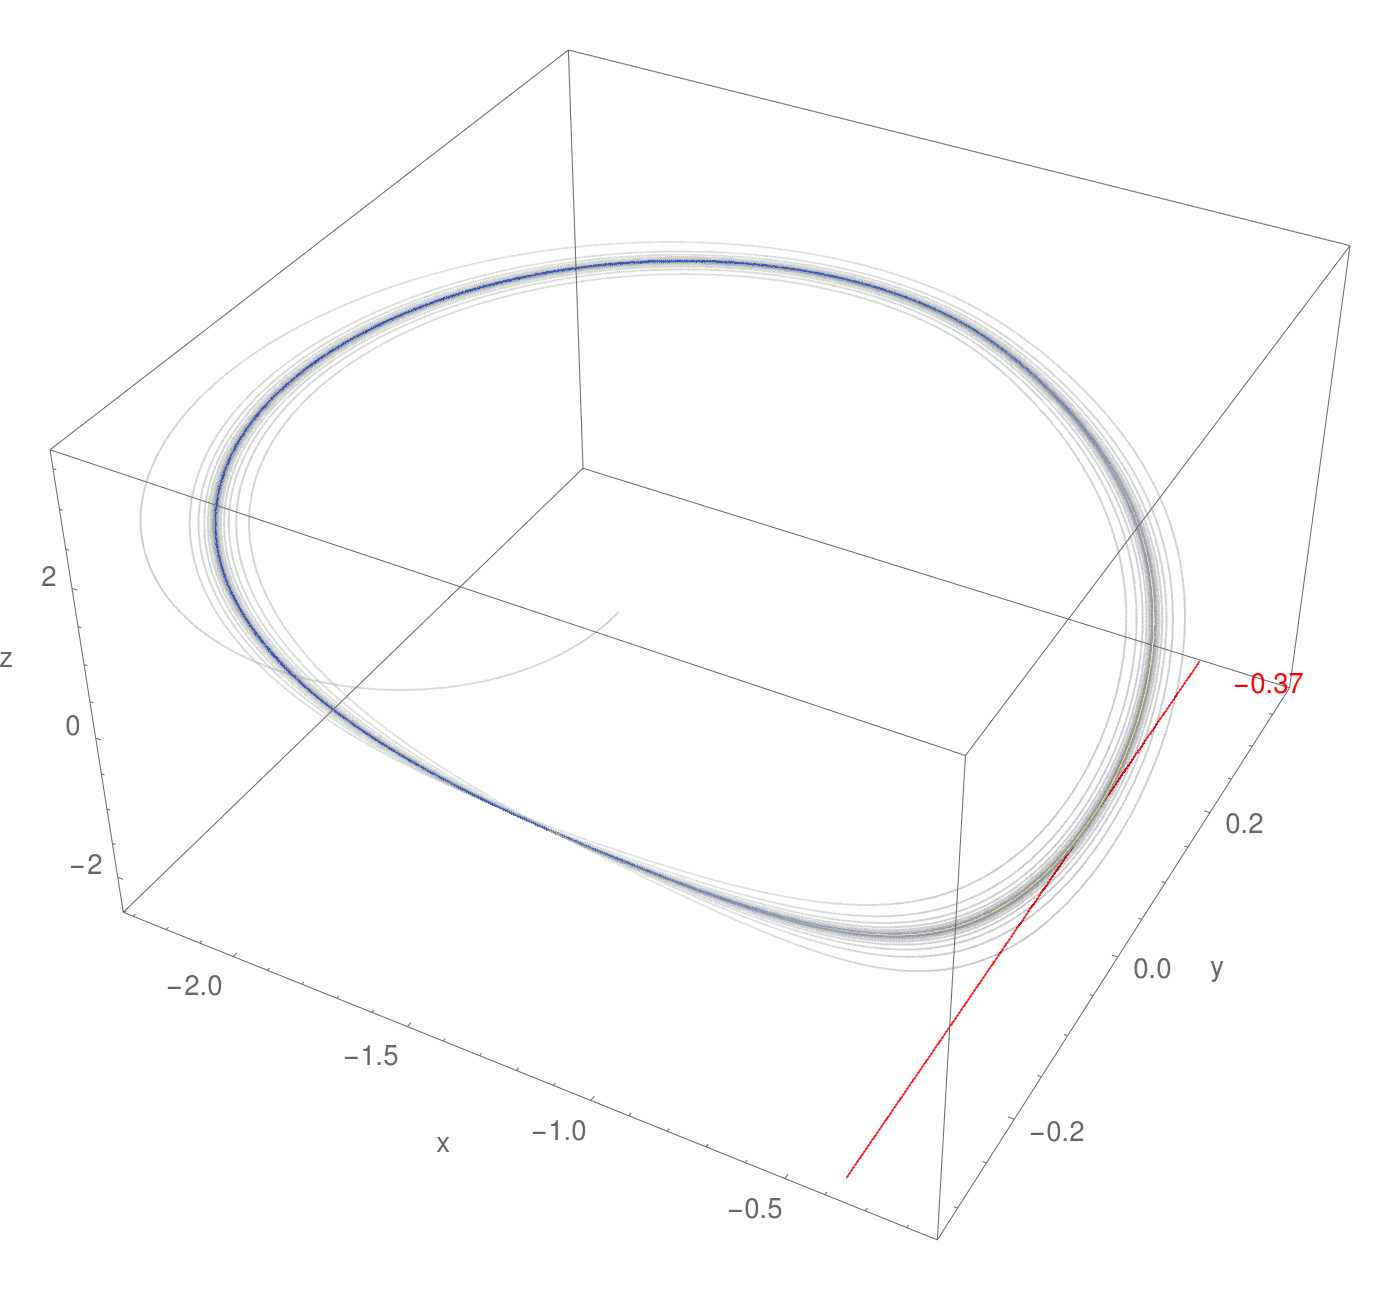
\includegraphics[height=0.45\textheight]{controllers/chua-circuit/Limited-chua-circuit-x-softness-0-5--0-37-convergence.png}
\caption[Figure of period 1 limit cycle]{Figure of period 1 limit cycle in the uppermost scroll using a self limiter with value 0.5.}
\label{figure:x-0.5-1-limit-cycle-upperscroll-trajectory}
\end{figure}

Pushing the limiter further into the negative limit values, one can again observe the plane rotation and the spiralling towards the uppermost scroll. %
%
Further limiting can suppress the progression of the trajectory entirely. %
%
The trajectory tries to spiral back into the uppermost scroll within limiter window \([-1,-4[\), but the radius of the spiral gets so small that the maximum precision of Mathematica is reached with limiter values \(<-4\).
%
Therefore the resulting trajectory starts to be discretized by the limited precision.

\begin{figure}[H]
\centering
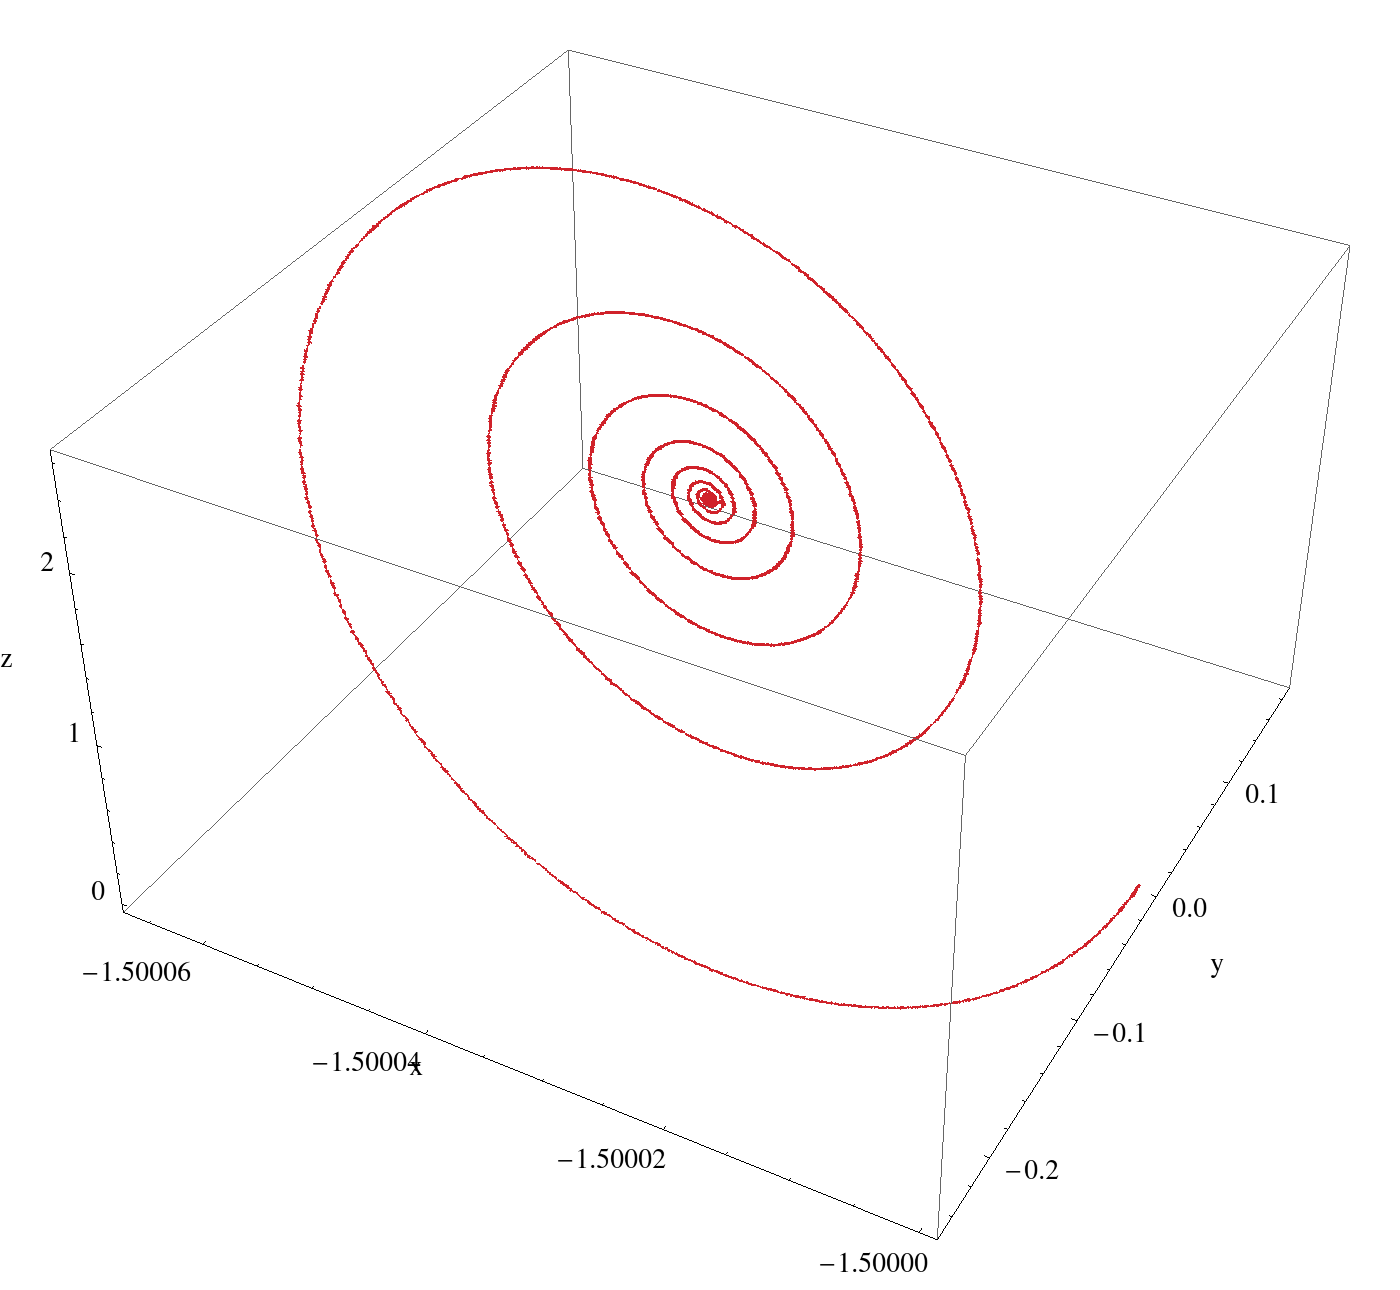
\includegraphics[height=0.45\textheight]{controllers/chua-circuit/Limited-chua-circuit-x-softness-0-5--4-convergence.png}
\caption[Figure showing discretization artifacts]{Figure of discretization artifacts in the uppermost scroll using a self limiter with value 0.5.}
\label{figure:x-0.5-discretization}
\end{figure}

\subsection{Chaotic Chua Circuit Controller}
% rev. 3

\begin{figure}[H]
\centering
\begin{tikzpicture}
% classes
\tikzstyle{root} = [draw=black!80, thick,minimum width=1.5cm,minimum height=1cm, circle, fill=black!20]
\tikzstyle{class1} = [minimum width=3cm, minimum height=2cm,draw=black!80, thick, fill=blue!5, rounded corners, rectangle]
\tikzstyle{class2} = [minimum width=2.5cm,minimum height=0.2cm, rounded corners,rectangle, fill=orange!80]
\tikzstyle{class3} = [minimum width=2.5cm,minimum height=0.2cm, rounded corners,rectangle, fill=red!80]

%###############################################
% parameter list above
%###############################################

%###############################################
% chaos symbol
%###############################################

%###############################################
% external chaotic output
%###############################################

%###############################################
% internal controller state
%###############################################

\end{tikzpicture}


\caption[The chaotic chua controller]{The specification of the chaotic chua controller, its internal state and output signal. The internal state of the chaotic chua controller is three dimensional because the Chua circuit's equations are defined using three dimensions. The output signal is chosen to be the z dimension of the internal state and is therefore only one dimensional. The controller state and output are shown for the unlimited condition and an example of limited condition. The example limitation leads to a period two limit cycle. If the chaotic chua circuit controller is mutated during the mutation step of the simulator, the parameters are chosen from a uniform distribution out of the respective intervals.}
\label{figure:chua-controller}
\end{figure}

The chaotic controller used to control a single DoF in a joint of a creature is driven internally by the Chua circuit examined above. %
%
The Chua circuit's parameters are kept constant to keep the parameter space for the evolution small, also there exist many parameter conditions that do not lead to a chaotic ground state. %
%
Only the initial conditions are chosen randomly within the bounding box \((x,y,z) \in ([-2,2],[-2,2],[-2,2])\) and the integration step is chosen randomly so that \(\text{\textit{integration step}} \in [0.001,10]\). %
%
During a mutation of the chaotic chua circuit controller, the initial conditions and the integration step are chosen anew from a uniform distribution out of the respective intervals.%
%
Even though the integration step can vary from controller to controller, the base integration step, is kept constant at \(\text{\textit{integration base}} = 0.0005\). %
%
The integration step then is performed by calculating small sub-steps of size of the \textit{base integration step} until a smaller, residual integration step is left to calculate. %
%
Thereby, variable size integration speeds can be performed, but the actual base integration step is kept constant. %
%
The numerical integration again is performed using a Runge-Kutta order 6 integration scheme run in real-time. %
%
However, in the creature's controller, the simple limiter is not directly applied as in the experiment above, but it will be tested if the controller output can be limited by the joint morphology, so that periodic motion emerges not in the controller, but in the joint. %
%
If this does not prove to be successful, a feedback to the chaotic system will be implemented which limits it according to the current state of the controlled joint. %

\end{document}